\chapter{Use cases with Simplified tools}


%-------------------------------------------------------------------
%-------------------------------------------------------------------
%-------------------------------------------------------------------

\section{The Vincennes data set}

%-------------------------------------------------------------------

\subsection{Description of the data set}
\label{Vincennes:DataSet}

On {\tt micmac\_data/ExempleDoc/} the directory {\tt Vincennes} contains
$106$ images of the Vincennes' castle \footnote{they are low resolution images
to limit the  downloading time}. This data set illustrate how
the tools described here can be used to achieve a typical architectural task:
compute for each of the main facade an ortho photo, these ortho photo
must be referenced in the same coordinate system.  Although the ortho-cylindrical
option for geometry described to process this acquisition seems a very specific
and narrow technical case, practically it corresponds to very current case
for facade processing.


The $106$ images of Vincennes' data set are organized in $4$ subset :


\begin{itemize}
   \item  images {\tt Face1.*} correspond to the first facade;
   \item  images {\tt Face2.*} correspond to the second facade;
   \item  images {\tt  Lnk12.*} images acquired to make the link between
           the two facades;
   \item  images {\tt  Calib.*} acquired to have easily a first
           calibration.
\end{itemize}

Note that, \emph{before any processing}, the images have been renamed taking
into account the acquisition structure. It is highly recommended to do the
same thing before processing data sets having some complexity. It avoids
the creation of tricky regular expression. These images are jpeg low resolution
images to limit the bandwidth when one upload the data, but of course in
real case the full resolution raw image will be preferred.


\begin{figure}
\begin{center}
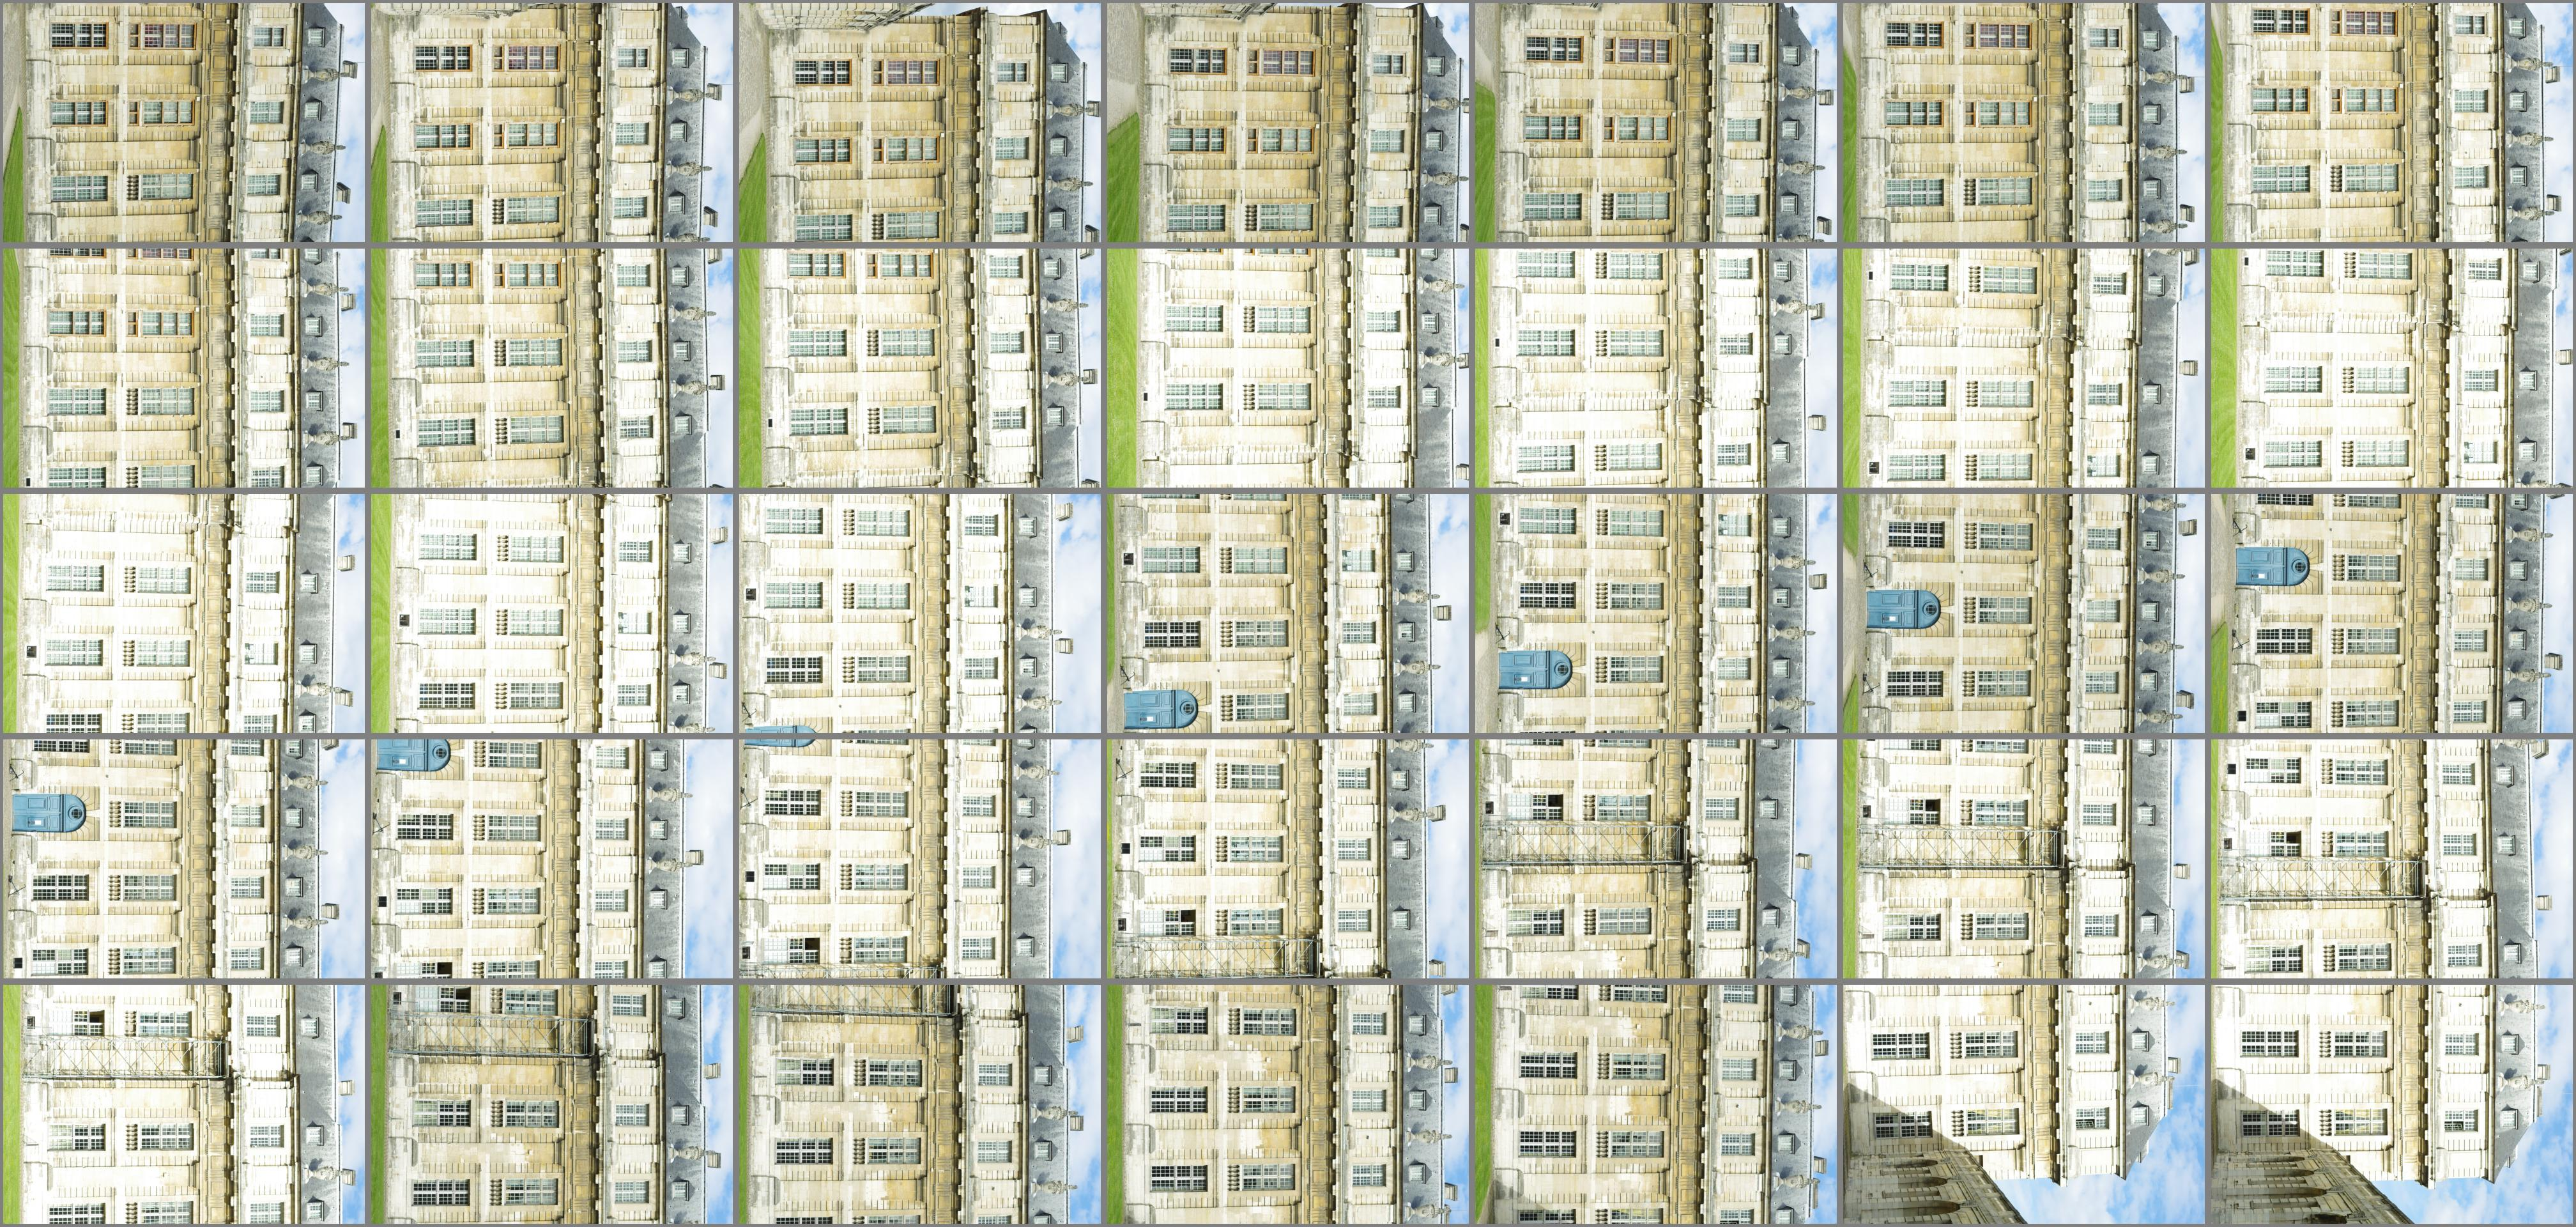
\includegraphics[width=120mm]{FIGS/Vincennes/Planche-F1.jpg}

\vspace{0.3cm}
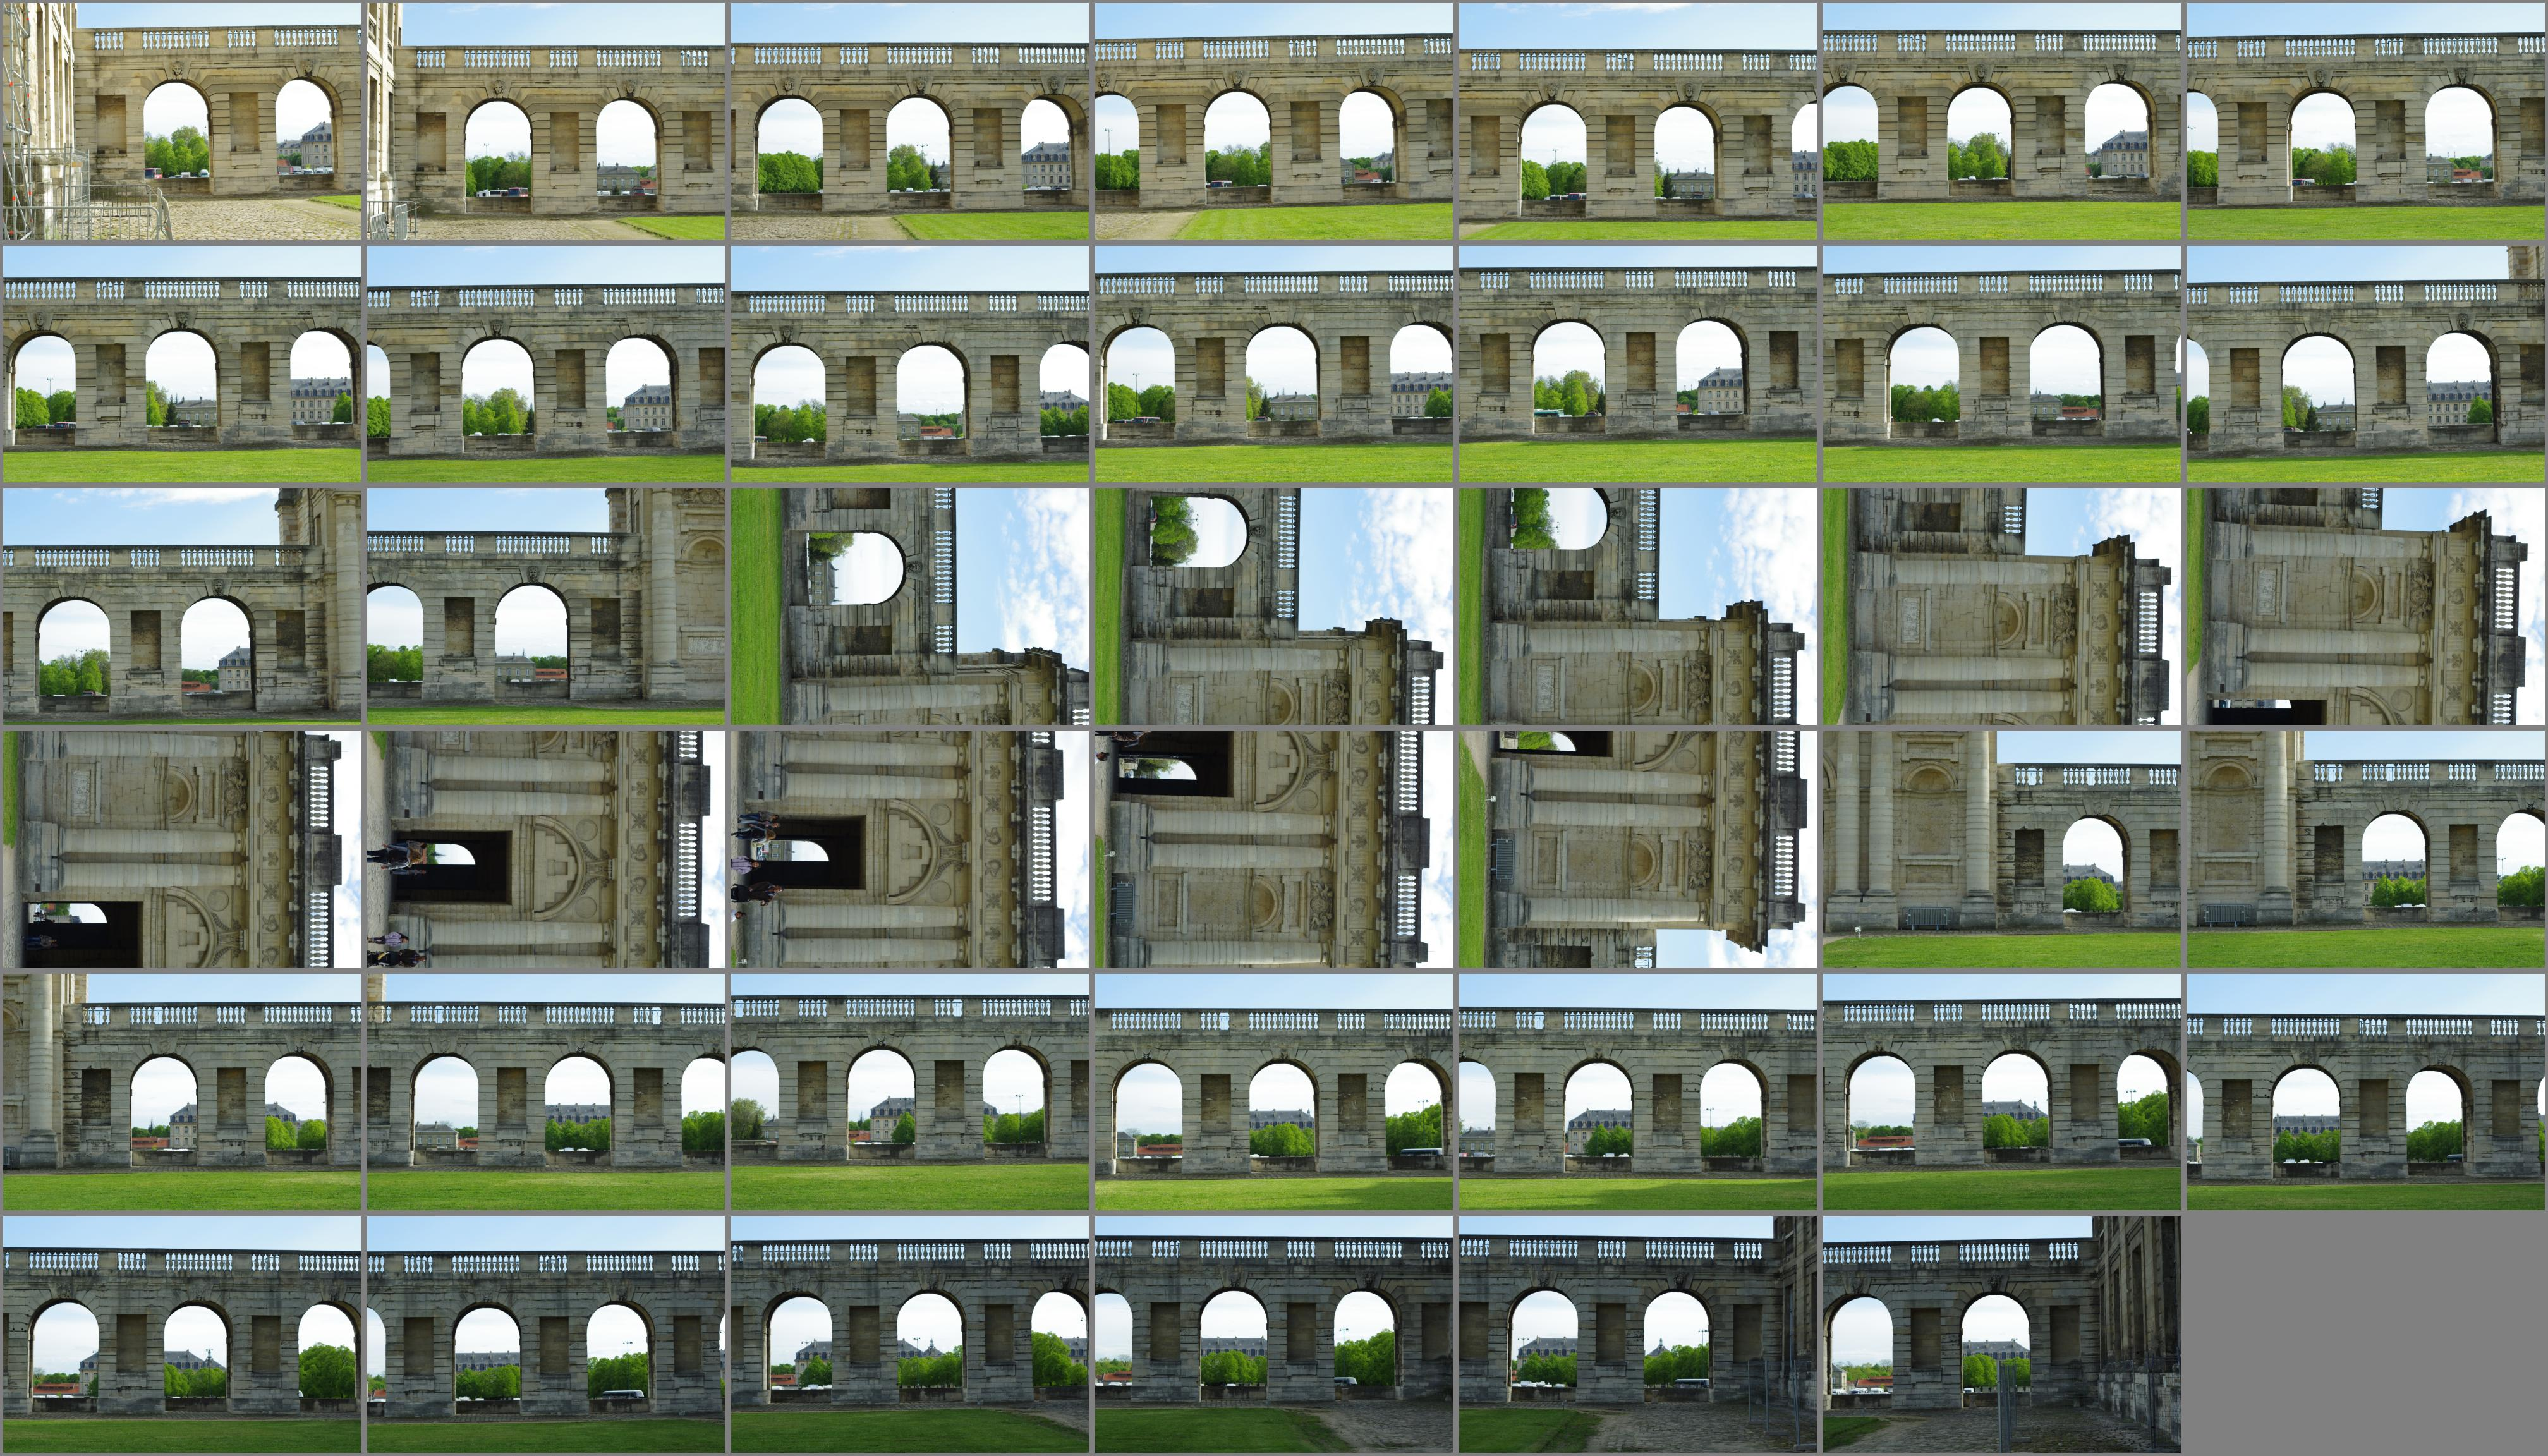
\includegraphics[width=120mm]{FIGS/Vincennes/Planche-F2.jpg}

\vspace{0.3cm}
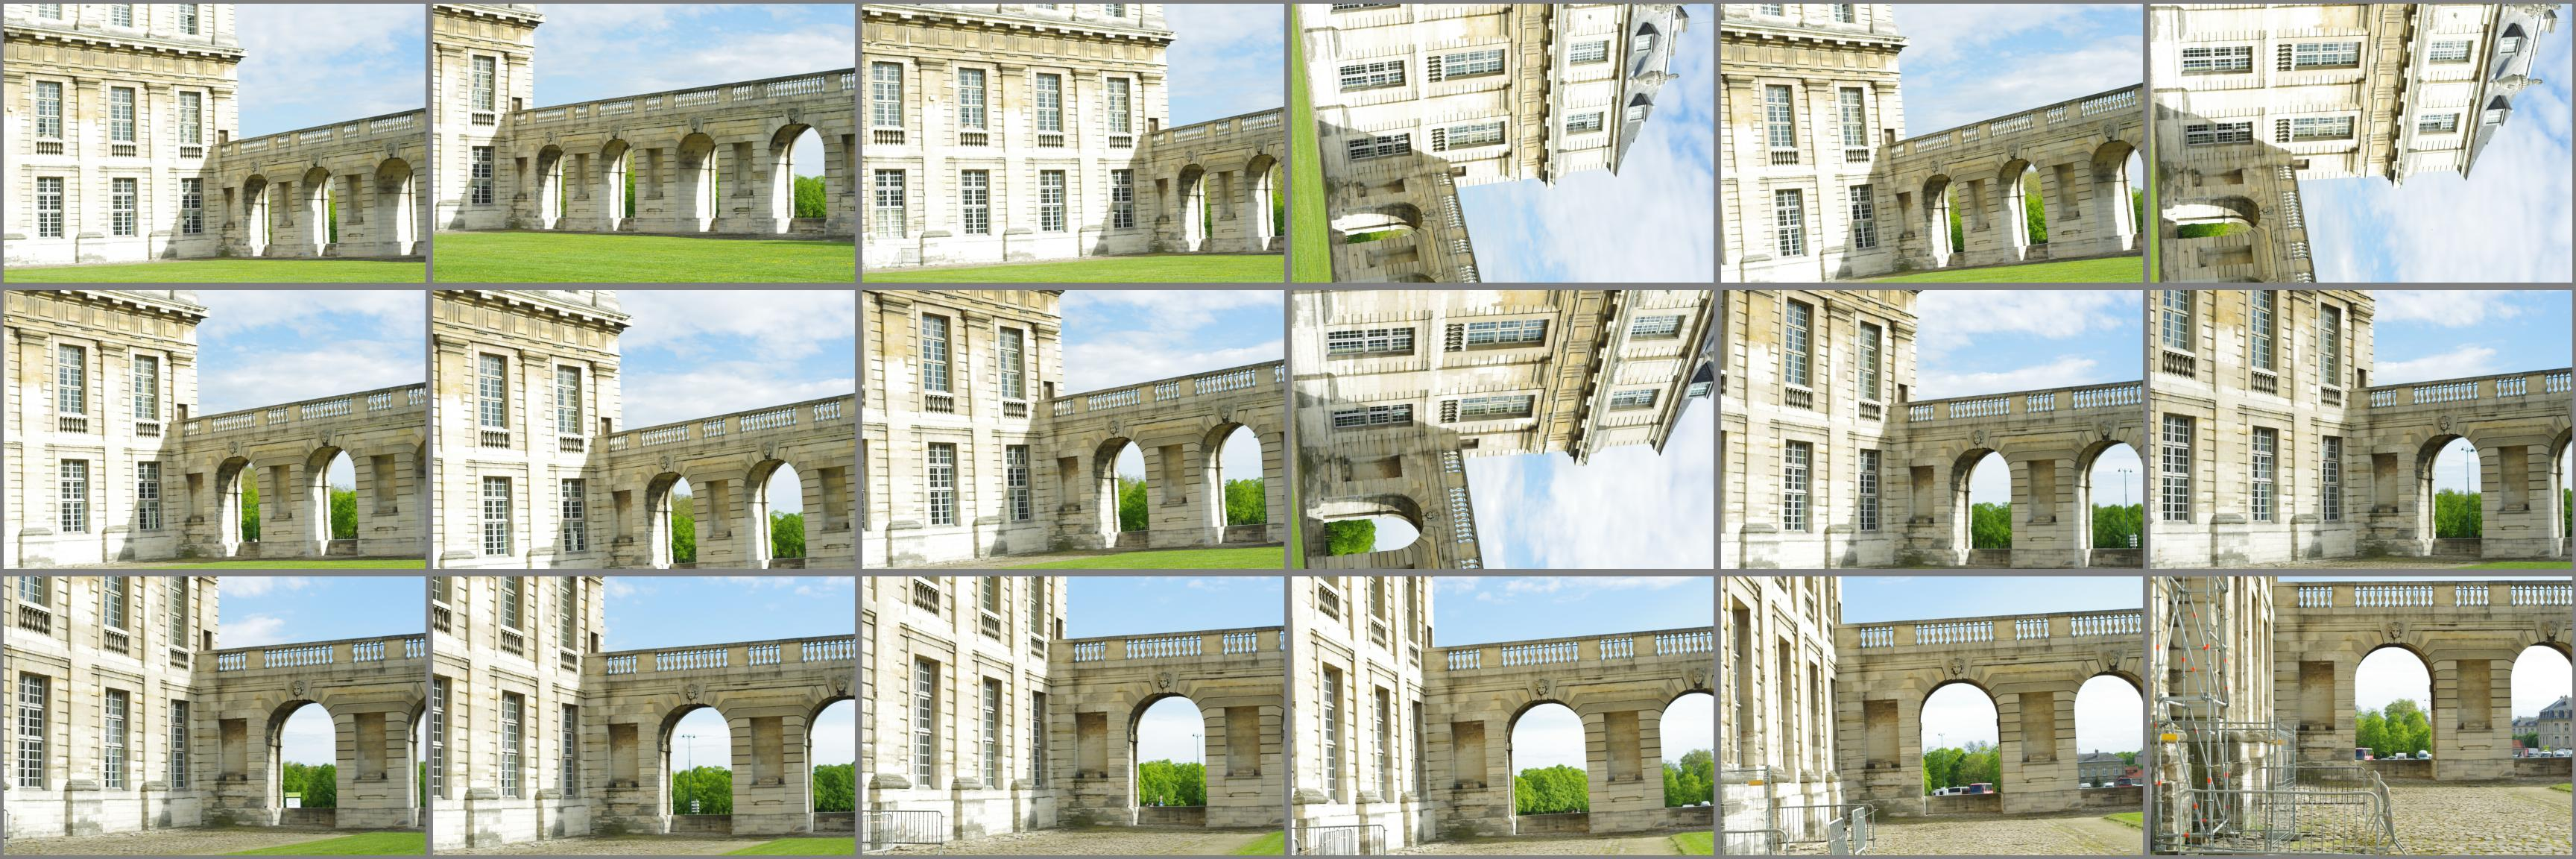
\includegraphics[width=120mm]{FIGS/Vincennes/Planche-Lnk.jpg}

\vspace{0.3cm}
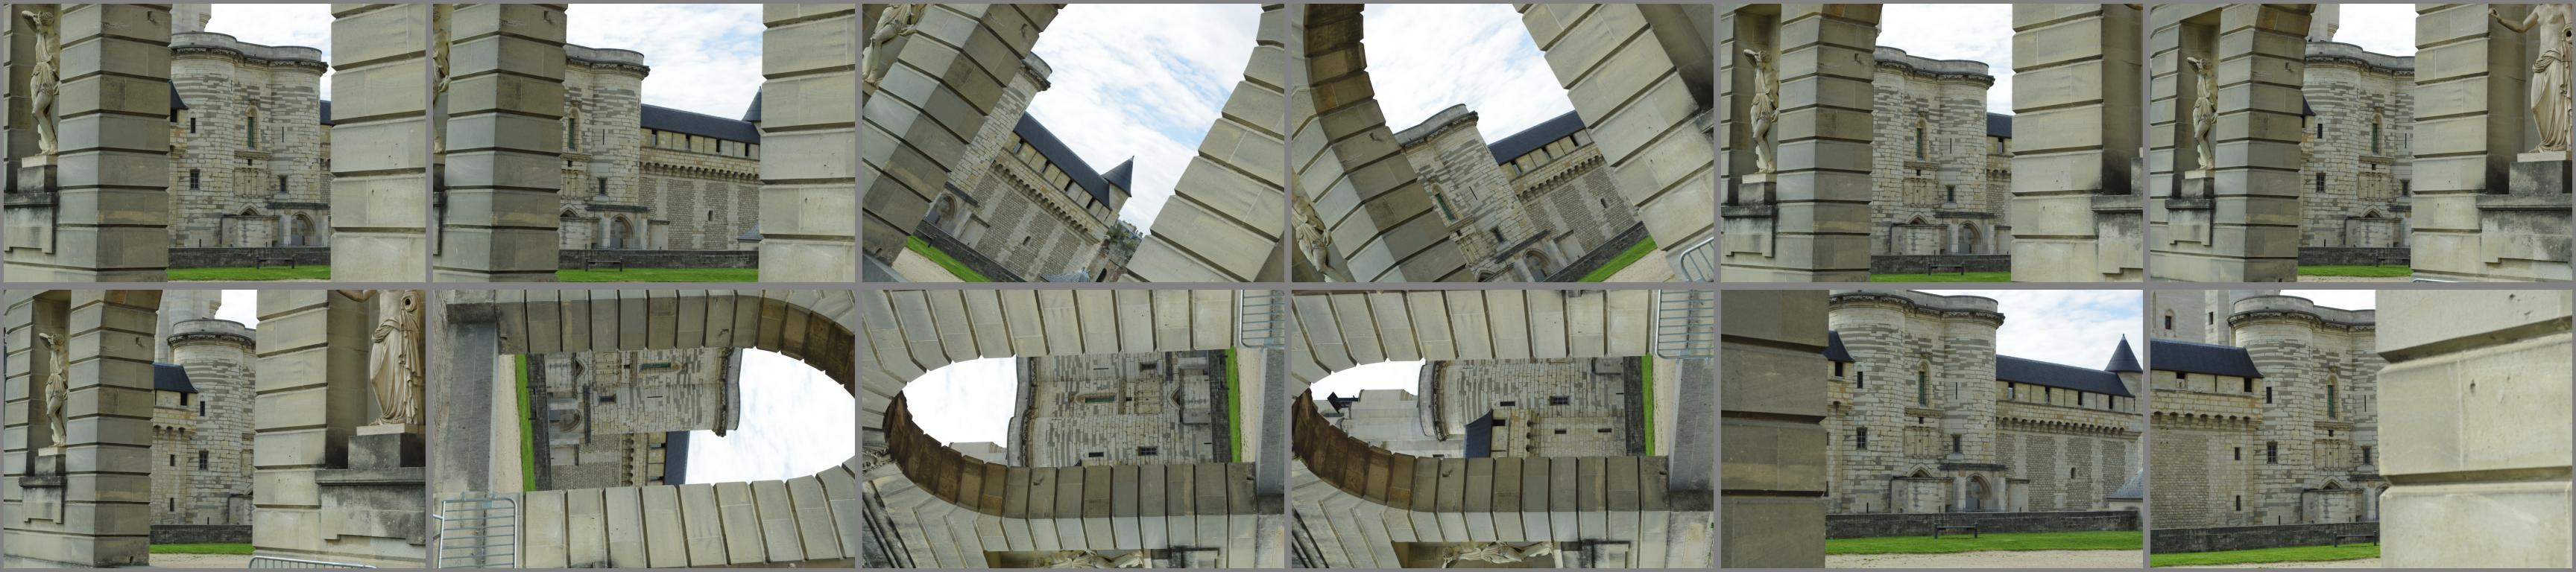
\includegraphics[width=120mm]{FIGS/Vincennes/Planche-Calib.jpg}
\end{center}
\caption{Image of Vincenne's data set : Face1, Face2, Lnk12 and Calib }
\label{FIG:Glob:Vincenne}
\end{figure}




The file {\tt  ExeCmd.txt} contains all the commands that we will need to process these images.


%-------------------------------------------------------------------

\subsection{Computing tie points and orientations}

    %  -  -  -  -  -  -  -  -  -  -  -  -

\subsubsection{Tie points}

The computation of tie points and relative orientation is quite
classic now.

For tie points we want to compute:

\begin{itemize}
   \item  points  between all pairs of calibration data set;
   \item  points  of \emph{Face1} and \emph{Face2} using the linear structure of
          the acquisition;
   \item  points  between \emph{Lnk12} and connected subset of  \emph{Face1} and \emph{Face2};
\end{itemize}

This is done by :

\begin{verbatim}
Tapioca All  "Calib-IMGP[0-9]{4}.JPG" 1000
Tapioca Line "Face1-IMGP[0-9]{4}.JPG" 1000 5
Tapioca Line "Face2-IMGP[0-9]{4}.JPG" 1000 5
Tapioca All  "((Lnk12-IMGP[0-9]{4})|(Face1-IMGP529[0-9])|(Face2-IMGP531[0-9])).JPG" 1000
\end{verbatim}

    %  -  -  -  -  -  -  -  -  -  -  -  -

\subsubsection{Relative orientation}

Then we want to make a first calibration with the calibration data set, and
use this calibration as an initial value to the global orientation of
\emph{Face1},  \emph{Face2} and \emph{Lnk12}. This is done by :

\begin{verbatim}
Tapas RadialStd "Calib-IMGP[0-9]{4}.JPG" Out=Calib
Tapas RadialStd "(Face1|Face2|Lnk12)-IMGP[0-9]{4}.JPG" Out=All InCal=Calib
\end{verbatim}

    %  -  -  -  -  -  -  -  -  -  -  -  -

\subsubsection{Optional, absolute orientation}

Finally, we want to transform the orientation from an arbitrary relative
orientation to some physically based orientation. If we have some ground
control points, this can be done using the {\tt GCPBascule} command (see~\ref{Sec:GCPBascule}) . To
generate orientation in {\tt Ori-Ground} :

\begin{verbatim}
GCPBascule  "(Face1|Face2|Lnk12)-IMGP[0-9]{4}.JPG" All Ground Mesure-TestApInit-3D.xml\
 Mesure-TestApInit.xml
\end{verbatim}

    %  -  -  -  -  -  -  -  -  -  -  -  -

\subsubsection{Optional, scene-based orientation}

Alternatively, if we do not have any GCP and want to put the data in an orientation
having some physical meaning, we can use the {\tt SBGlobBascule} command (see~\ref{ScBas:Basc}) :

\begin{verbatim}
SBGlobBascule "(Face1|Face2|Lnk12)-IMGP[0-9]{4}.JPG" All MesureBascFace1.xml  Glob \
    PostPlan=_MasqPlanFace1  DistFS=2.0 Rep=ij
\end{verbatim}

There is a new option {\tt Rep=ij}, the meaning of this option is :
\label{SGB:Rep}

\begin{itemize}
   \item it is a string that describe a repair;
   \item it must contain $2$ symbols, each symbols can be in \emph{\{i,-i,j,-j,k,-k\}} and describe a vector;
   \item the global orientation with be such that in the final orientation the line
         defined by {\tt Line1-Line2} is aligned on first vector, and the normal to the plane is aligned on second vector;
   \item here in final orientation $i$ will be the horizontal of the wall and $j$ will be the
         normal to the wall, consequently $k=i\wedge j$ will be the vertical;
\end{itemize}


%-------------------------------------------------------------------
\subsection{Matching}


    %  -  -  -  -  -  -  -  -  -  -  -  -
\subsubsection{"Standard" option}

The "standard pipeline" for generating an ortho photo of facade,
as seen in~\ref{Simp:Tool:One}, is for each facade :

\begin{itemize}
   \item compute a local repair to define the facade with {\tt RepLocBascule};
   \item compute a rectified image with {\tt Tarama};
   \item make the matching with {\tt Malt};
   \item generate the ortho image with {\tt  Tawny};
\end{itemize}

This can be done by the succession of commands:

\begin{verbatim}
RepLocBascule  "(Face1)-IMGP[0-9]{4}.JPG" Ground  MesureBascFace1.xml Repere-F1.xml\
       PostPlan=_MasqPlanFace1
Tarama  "(Face1)-IMGP[0-9]{4}.JPG" Ground  Repere=Repere-F1.xml  Out=TA-F1 Zoom=4
Malt Ortho  "(Face1)-IMGP[0-9]{4}.JPG"  Ground  Repere=Repere-F1.xml  \
                     SzW=1 ZoomF=1  DirMEC=Malt-F1 DirTA=TA-F1
Tawny Ortho-Malt-F1/
\end{verbatim}

The results are quite deceiving !!! Figure~\ref{FIG:Pb:Vincenne} illustrate the
encountered problem :

\begin{itemize}
    \item on first line, the ortho photo; it suffer several problem; the main problem
         are located on the roof (due to bad incidence angles) and on horizontal lines;

    \item on second line, a snapshot from Meshlab, showing the camera position;
          it illustrates the fact that in this acquisition all the camera centers are
         located on the same line;

    \item the third line, focus on the matching problem  that occurs on linear detail that
          are parallel to the line of acquisition;
\end{itemize}


\begin{figure}
\begin{center}
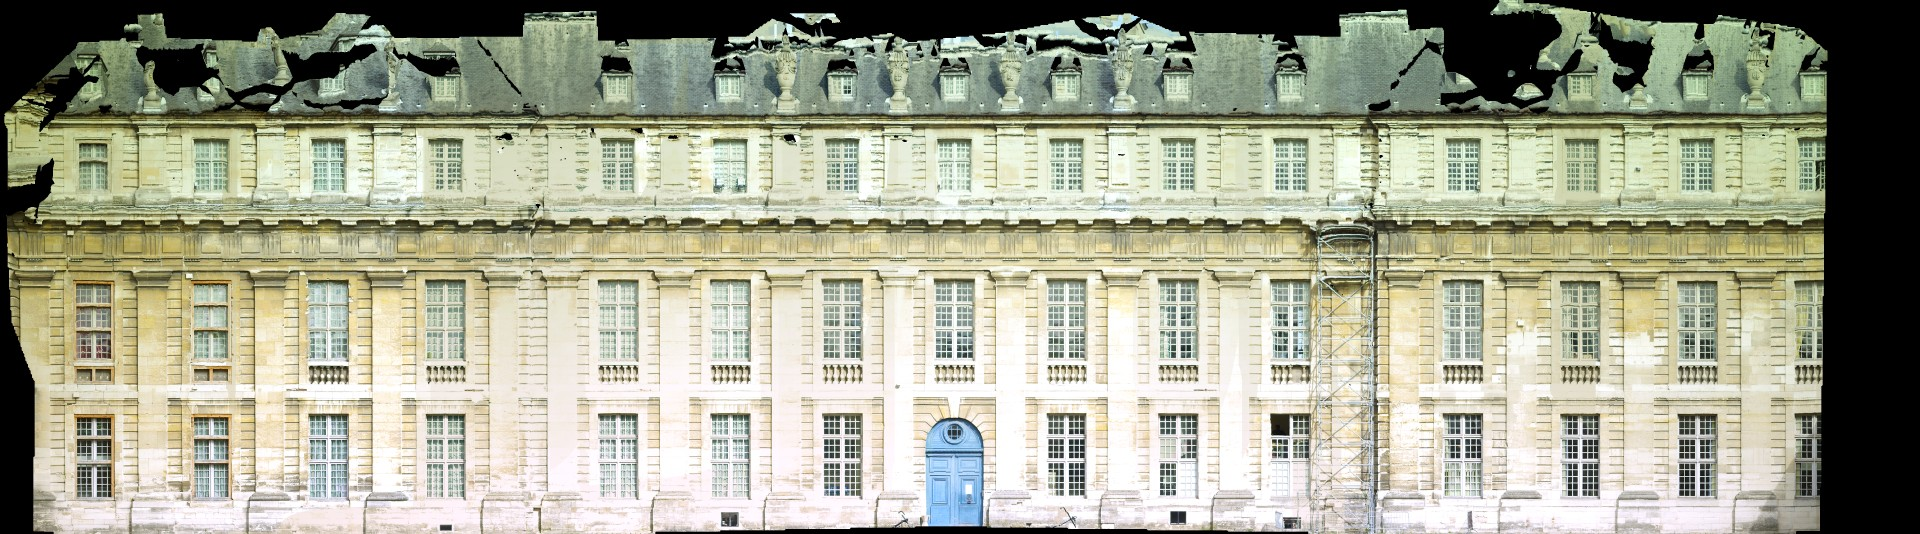
\includegraphics[width=160mm]{FIGS/Vincennes/Ortho-Moche.jpg}

\vspace{0.3cm}
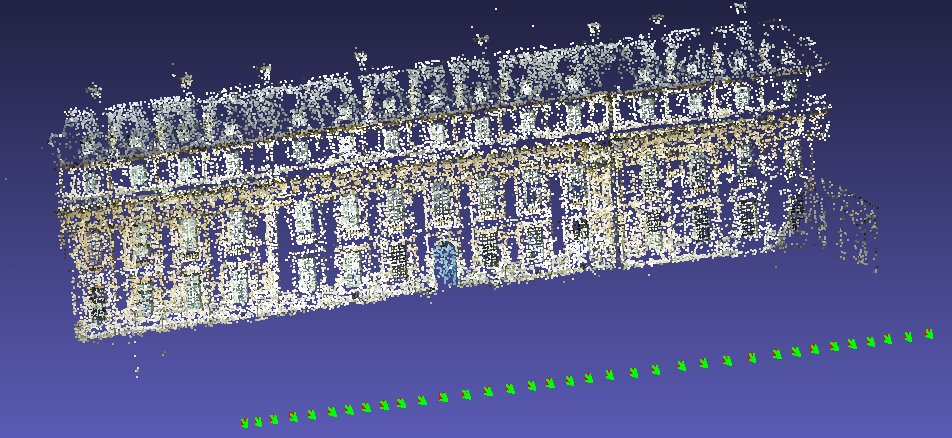
\includegraphics[width=160mm]{FIGS/Vincennes/CamFace1.jpg}

\vspace{0.3cm}
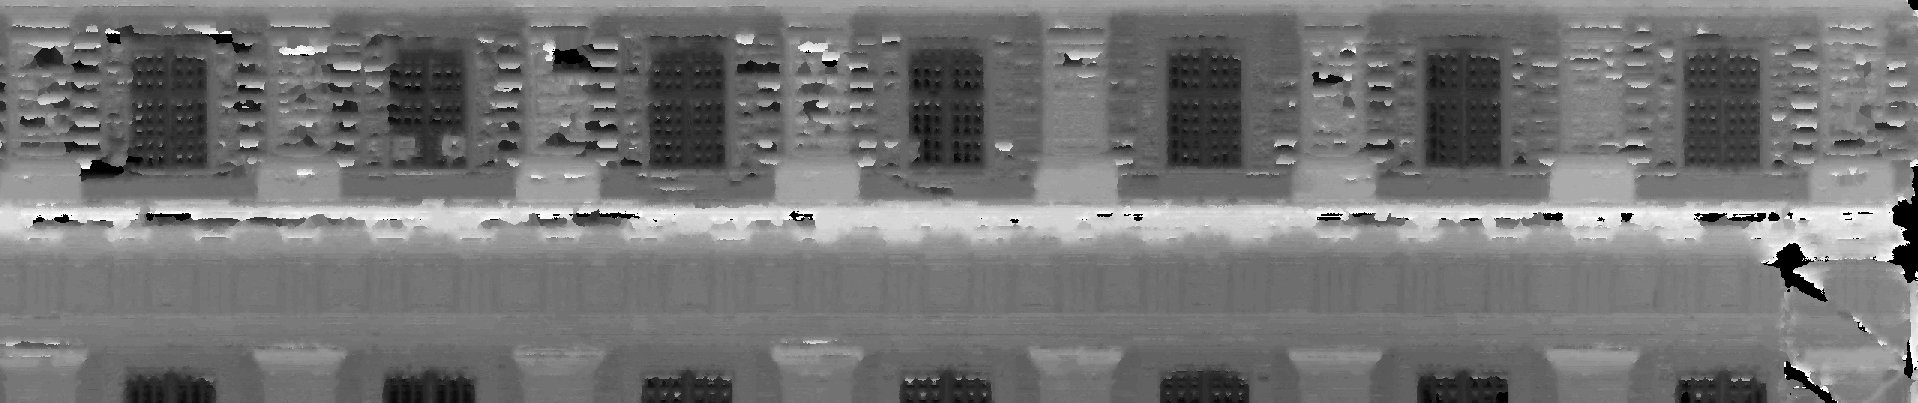
\includegraphics[width=160mm]{FIGS/Vincennes/MNT-Moche.jpg}

\end{center}
\caption{Problem with standard processing on Vincennes Facade : low quality ortho photo,
aligment of cameras, poor dept map especially for linear structure parallel to camera alignment}
\label{FIG:Pb:Vincenne}
\end{figure}


    %  -  -  -  -  -  -  -  -  -  -  -  -
\subsubsection{"Ortho-cylindrical" option}

Intuitively it  is obvious that when the camera center are all aligned on the same line,
the matching problem is  ambiguous for line parallel to the acquisition, consequently
the quality of result is poor.
Obviously, the default would decrease (in fact disappear) if the camera were not
aligned, using an UAV or a scaffolding , we could have an optimal geometry similar
to aerial acquisition. But it is not always possible to have such material and, for economical reason,
it would be interesting to be able to obtain a relatively good quality ortho photo even when
all the camera are aligned.

In fact for theoretical reasons described in~\cite{Penard},
this problem are  much more important in ground geometry than in image geometry.
With the option we have seen until now, we have basically this alternative:

\begin{itemize}
   \item  use the ground geometry with a simple process but obtain bad quality results such those of
          figure~\ref{FIG:Pb:Vincenne};

   \item  use the image geometry with  good results but have a complicated workflow with many depth map
          that must be merged.
\end{itemize}


With such acquisition, the ortho-cylindrical geometry combine the benefit of these
two geometries. Intuitively this geometry is equivalent to the geometry of a virtual push-broom
camera, the line of this virtual push-broom being the line on which are located the
camera center. More formally :


\begin{itemize}
   \item  let  $X,Y,Z$ be a coordinate system such that $Y=0$ be approximately the line on which the camera
          are located, and $Z=D$ be approximately the plane of the wall;

   \item  let  $U,V,L$ be the coordinate system defined by
\begin{itemize}
    \item  $U= D \tan^{-1} (\frac{X}{Z})$
    \item  $V=Y$ and $L=Z$;
\end{itemize}
   \item   we  will then compute the DSM as a function $L= F(U,V)$.
\end{itemize}

To use this geometry, we just need to set {\tt OrthoCyl=true} in the command {\tt RepLocBascule} :

\begin{verbatim}
RepLocBascule  "(Face1)-IMGP[0-9]{4}.JPG" Ground  MesureBascFace1.xml Ortho-Cyl1.xml\
   PostPlan=_MasqPlanFace1 OrthoCyl=true
\end{verbatim}

With this option, {\tt RepLocBascule} will also compute, using least mean square,
the line that fit the best the alignment of camera perspective centers. If we take
a look at file {\tt Ortho-Cyl1.xml} we can see  this line coded by {\tt <P0>}
and {\tt <P1>}  (plus the previous local repair  {\tt <Repere>}) :

\begin{verbatim}
<XmlModeleSurfaceComplexe>
     <XmlOneSurfaceAnalytique>
          <XmlDescriptionAnalytique>
               <OrthoCyl>
                    <Repere>
                         <Ori>-0.00573  -2.7113574  -0.4521156 </Ori>
                         <Ox>  0.00029   0.9999998  -0.0003715 </Ox>
                         <Oy> -0.00043   0.0003716   0.9999998 </Oy>
                         <Oz>  0.99999  -0.0002960   0.0004372 </Oz>
                    </Repere>
                    <P0>30.392821 -2.720358 -0.438823</P0>
                    <P1>30.391561 -1.720359 -0.43974</P1>
                    <AngulCorr>true</AngulCorr>
               </OrthoCyl>
          </XmlDescriptionAnalytique>
          <Id>TheSurf</Id>
          <VueDeLExterieur>true</VueDeLExterieur>
     </XmlOneSurfaceAnalytique>
</XmlModeleSurfaceComplexe>
\end{verbatim}

    %  -  -  -  -  -  -  -  -  -  -  -  -
\subsubsection{Concrete use of "Ortho-cylindric" option}

It is then sufficient to give the file created by  {\tt RepLocBascule}
as an optional parameter to {\tt Tarama} and {\tt Malt} to compute
in the adequate geometry; for facade one, we can enter:


\begin{verbatim}
RepLocBascule  "(Face1)-IMGP[0-9]{4}.JPG" Ground  MesureBascFace1.xml Ortho-Cyl1.xml \
        PostPlan=_MasqPlanFace1 OrthoCyl=true
Tarama  "(Face1)-IMGP[0-9]{4}.JPG" Ground  Repere=Ortho-Cyl1.xml  Out=TA-OC-F1 Zoom=4
Malt Ortho  "(Face1)-IMGP[0-9]{4}.JPG"  Ground  Repere=Ortho-Cyl1.xml  \
                   SzW=1 ZoomF=1  DirMEC=Malt-OC-F1 DirTA=TA-OC-F1
Tawny Ortho-UnAnam-Malt-OC-F1/
\end{verbatim}

And for facade 2 :

\begin{verbatim}
RepLocBascule  "(Face2)-IMGP[0-9]{4}.JPG" Ground  MesureBascFace2.xml Ortho-Cyl2.xml \
     PostPlan=_MasqPlanFace2 OrthoCyl=true
Tarama  "(Face2)-IMGP[0-9]{4}.JPG" Ground  Repere=Ortho-Cyl2.xml  Out=TA-OC-F2 Zoom=4
Malt Ortho  "(Face2)-IMGP[0-9]{4}.JPG"  Ground  Repere=Ortho-Cyl2.xml  SzW=1 ZoomF=1  \
          DirMEC=Malt-OC-F2 DirTA=TA-OC-F2 NbVI=2
Tawny Ortho-UnAnam-Malt-OC-F2/
\end{verbatim}

Note some options of these commands:

\begin{itemize}
   \item in {\tt RepLocBascule}, the {\tt OrthoCyl=true} as described above;
   \item in {\tt Tarama}, the {\tt Out=TA-OC-F1} (and {\tt Out=TA-OC-F2}) to specify the
         directory of output; this is naturally to avoid that each call to {\tt Tarama} overwrite
         the result of previous calls;
   \item in {\tt Malt}, the {\tt DirTA=TA-OC-F1} to get the adequete entry from  {\tt Tarama}
         and {\tt Out=DirMEC=Malt-OC-F1} to specify the results; this change the place are written
         the results of matching, and also the result of individual ortho photo (here it will be
         {\tt Ortho-UnAnam-Malt-OC-F1/});
\end{itemize}


If the ortho-cylindrical geometry is "optimal" for computation, this is
generally not a proper geometry for the final user , so at the end of the process,
{\tt MicMac} generate an "un-anamorphosed" version of this depth map in
euclidean geometry.  For example on directory {\tt Malt-OC-F1/}, there
exists $9$ files {\tt Z\_NumX\_DeZoomY\_STD-MALT.tif} corresponding to
the different level of matching in ortho-cylindrical geometry,
and a single file {\tt Z\_Num1\_DeZoom1\_Malt-Ortho-UnAnam.tif}
corresponding to the eulidean version of the last file
( this is the version presented on second line of
figure~\ref{FIG:OK:Vincenne}).
Note that in general there will be very few hidden part on
ortho-cylindrical depth map; conversely, they are quite current on
euclidean version, but it is intrinsic to what we want to restituate
with such acquisition.
By default, the ortho photo are also generated in euclidean geometry
using the unanamorphosed depth-map. Here for example, they are
generated under {\tt Ortho-UnAnam-Malt-OC-F1/} and {\tt Ortho-UnAnam-Malt-OC-F2/}.


Figure~\ref{FIG:OK:Vincenne} present some results obtained after this process:

\begin{itemize}
    \item first line present the depth-map computed in ortho-cylindric geometry using
           color code;
    \item  second line, euclidean version of the depth map, remark the hidden part;

    \item  third line, ortho photo of facade.
\end{itemize}

\begin{figure}
\begin{center}
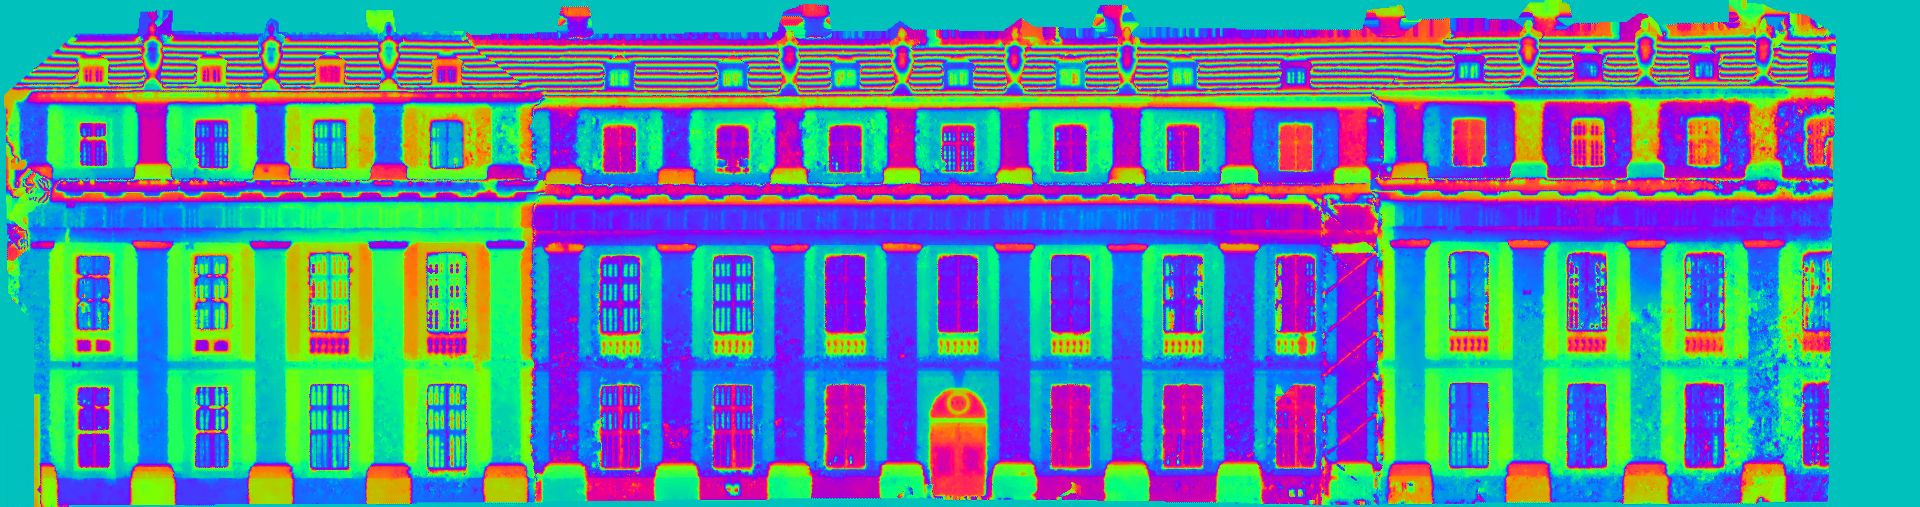
\includegraphics[width=160mm]{FIGS/Vincennes/MNE-OC.jpg}

\vspace{0.3cm}
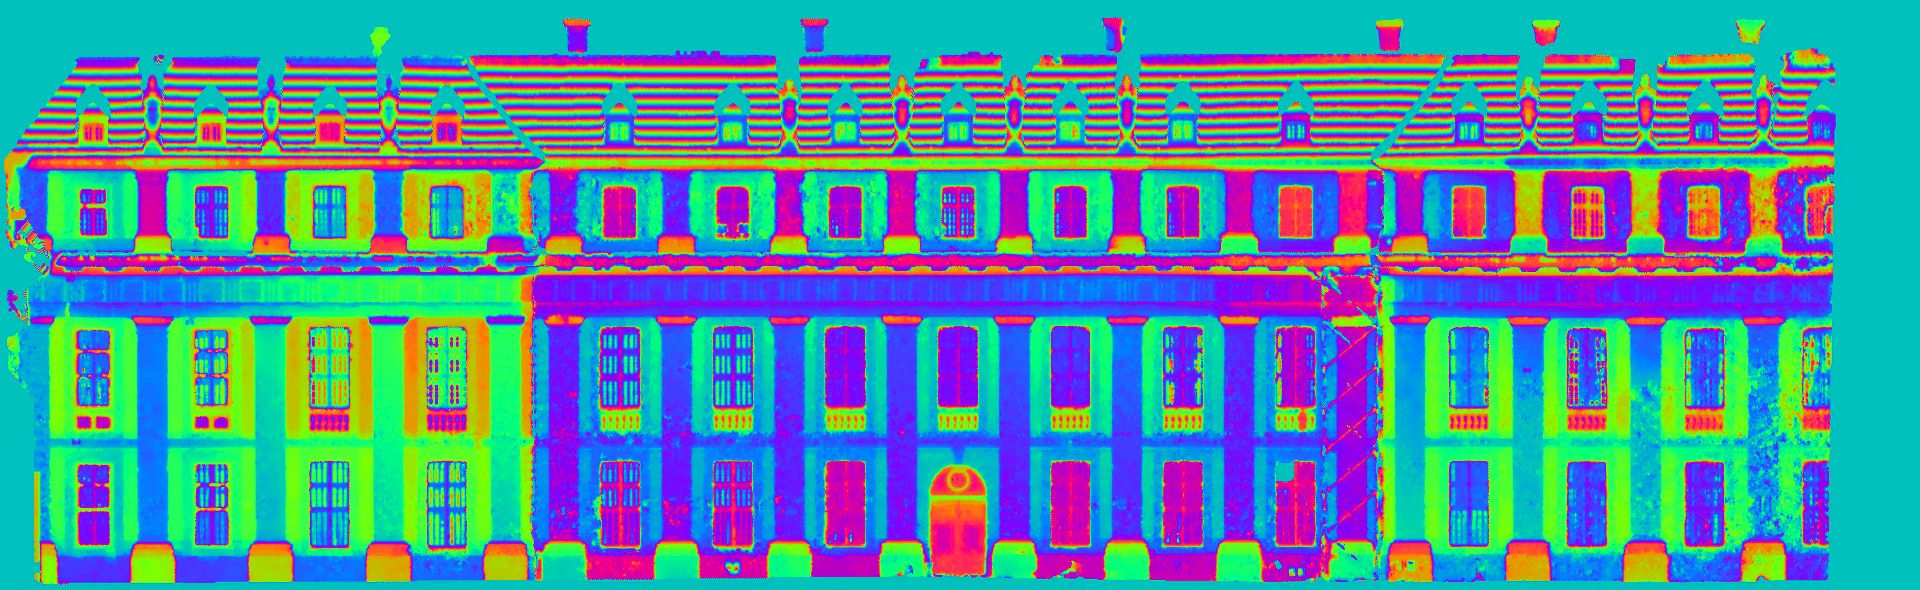
\includegraphics[width=160mm]{FIGS/Vincennes/MEN-Eucl.jpg}

\vspace{0.3cm}
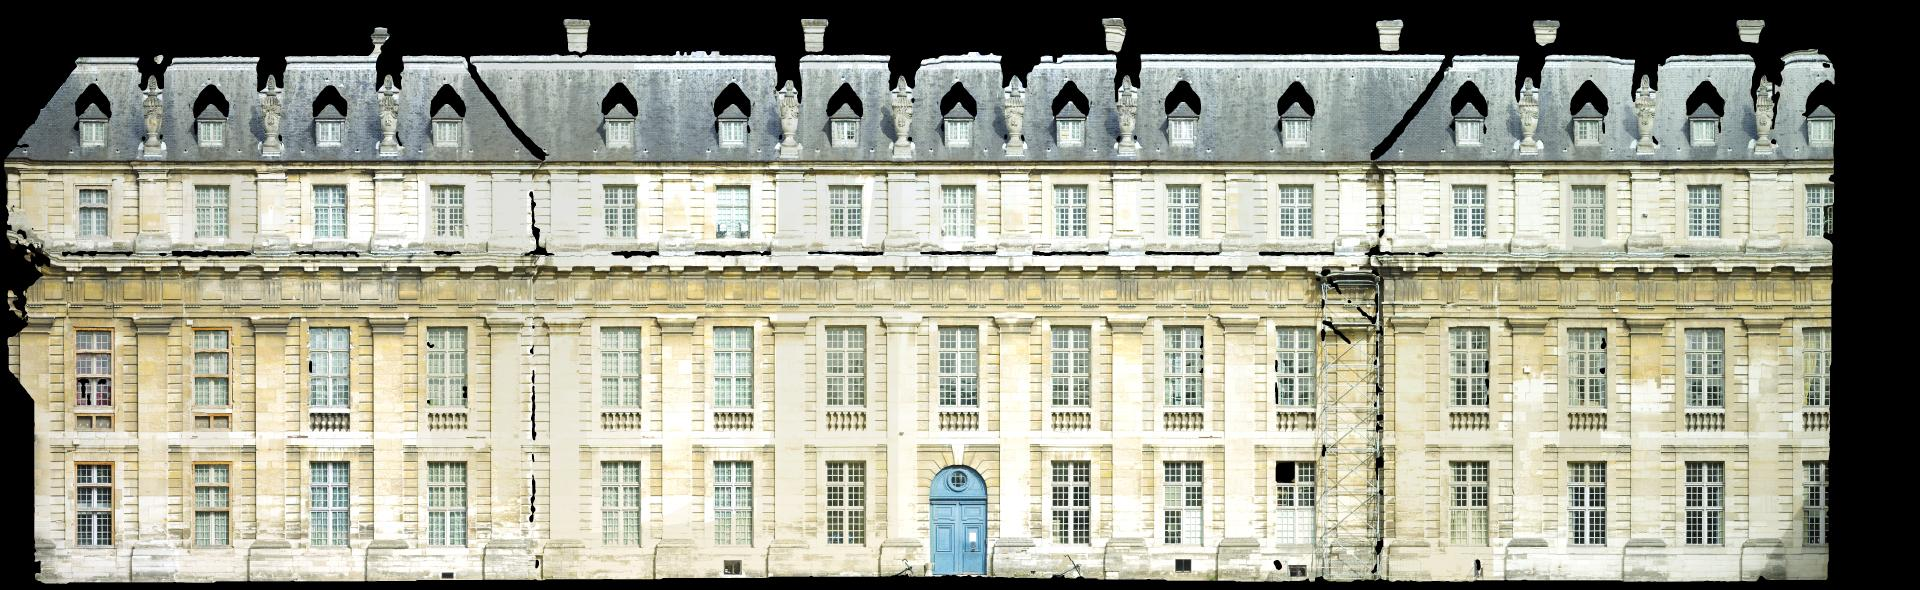
\includegraphics[width=160mm]{FIGS/Vincennes/Ortho-Eg-Test-Redr.jpg}

\end{center}
\caption{1-Depth map in ortho cylindric geometry, 2-The same, anamorphosed in euclidean
geometry, 3-Ortho photo in euclidean geometry}
\label{FIG:OK:Vincenne}
\end{figure}


Although all the tool described in this section are rather optimized
for ortho-photo generation, it is still possible to generate 3D cloud points.
As usual in ground geometry, we use the result of matching for the 3D and
the ortho-photo for textures.
For example:


\begin{verbatim}
Nuage2Ply Malt-OC-F1/NuageImProf_Malt-Ortho-UnAnam_Etape_1.xml \
      Attr=Ortho-UnAnam-Malt-OC-F1/Ortho-Eg-Test-Redr.tif Scale=3

Nuage2Ply Malt-OC-F2/NuageImProf_Malt-Ortho-UnAnam_Etape_1.xml \
      Attr=Ortho-UnAnam-Malt-OC-F2/Ortho-Eg-Test-Redr.tif Scale=3
\end{verbatim}

The meta data file {\tt NuageImProf\_Malt-Ortho-UnAnam\_Etape\_1.xml} contains
all the information relative to the local repair use for computation  (inside
the {\tt <RepereGlob>} balise):

\begin{verbatim}
<?xml version="1.0" ?>
<XML_ParamNuage3DMaille>
     <NbPixel>5972 1834</NbPixel>
     <PN3M_Nuage>
..
     </PN3M_Nuage>
     <RepereGlob>
          <Ori>-0.00573682224569793675 -2.71135741550217935 -0.452115668474152133</Ori>
          <Ox>0.000296255688442622397 0.999999887087029138 -0.000371562236912849938</Ox>
          <Oy>-0.000437158066873386052 0.000371691728275074906 0.999999835369028367</Oy>
          <Oz>0.999999860562685972 -0.000296093208240548543 0.000437268133301418503</Oz>
     </RepereGlob>
...
  <Orientation>
....
  </Orientation>
...
</XML_ParamNuage3DMaille>
\end{verbatim}

The point cloud are then generated in the same global repair and are
naturally mergeable as can be seen on figure~\ref{FIG:TroidD:Vincenne}.


\begin{figure}
\begin{center}
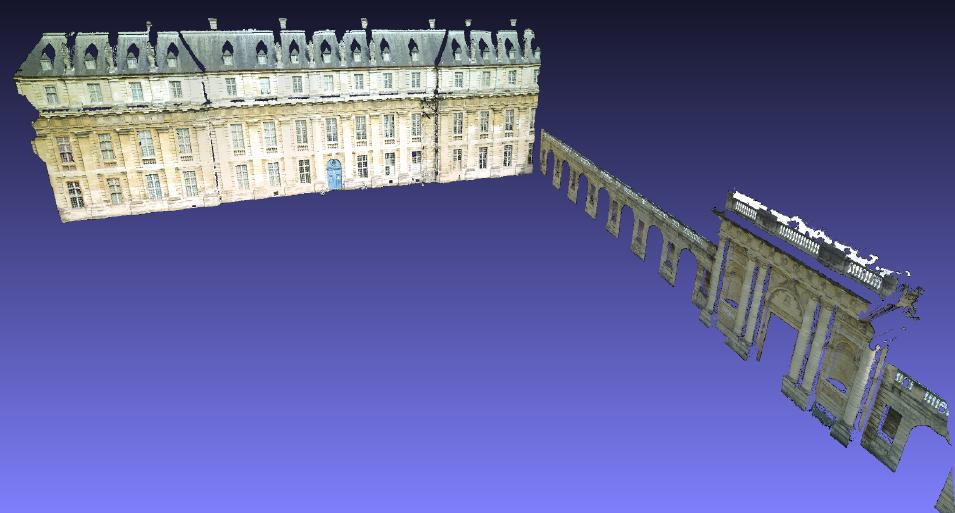
\includegraphics[width=160mm]{FIGS/Vincennes/Vinc3D.jpg}
\end{center}
\caption{Snapshot of two point clouds of the facade}
\label{FIG:TroidD:Vincenne}
\end{figure}

%-------------------------------------------------------------------
%-------------------------------------------------------------------
%-------------------------------------------------------------------

\section{The Saint-Michel de Cuxa data set}

%-------------------------------------------------------------------

\subsection{Description of the data set}
\label{Cuxa:DataSet}

On {\tt micmac\_data/ExempleDoc/} the directory {\tt MiniCuxha} contains
$48$ images of the St-Michel de Cuxa's abbey \footnote{they are low resolution images
to limit the  downloading time}. This data set illustrates how to
do a bundle adjustment with ground control points.

\begin{figure}[H]
\begin{center}
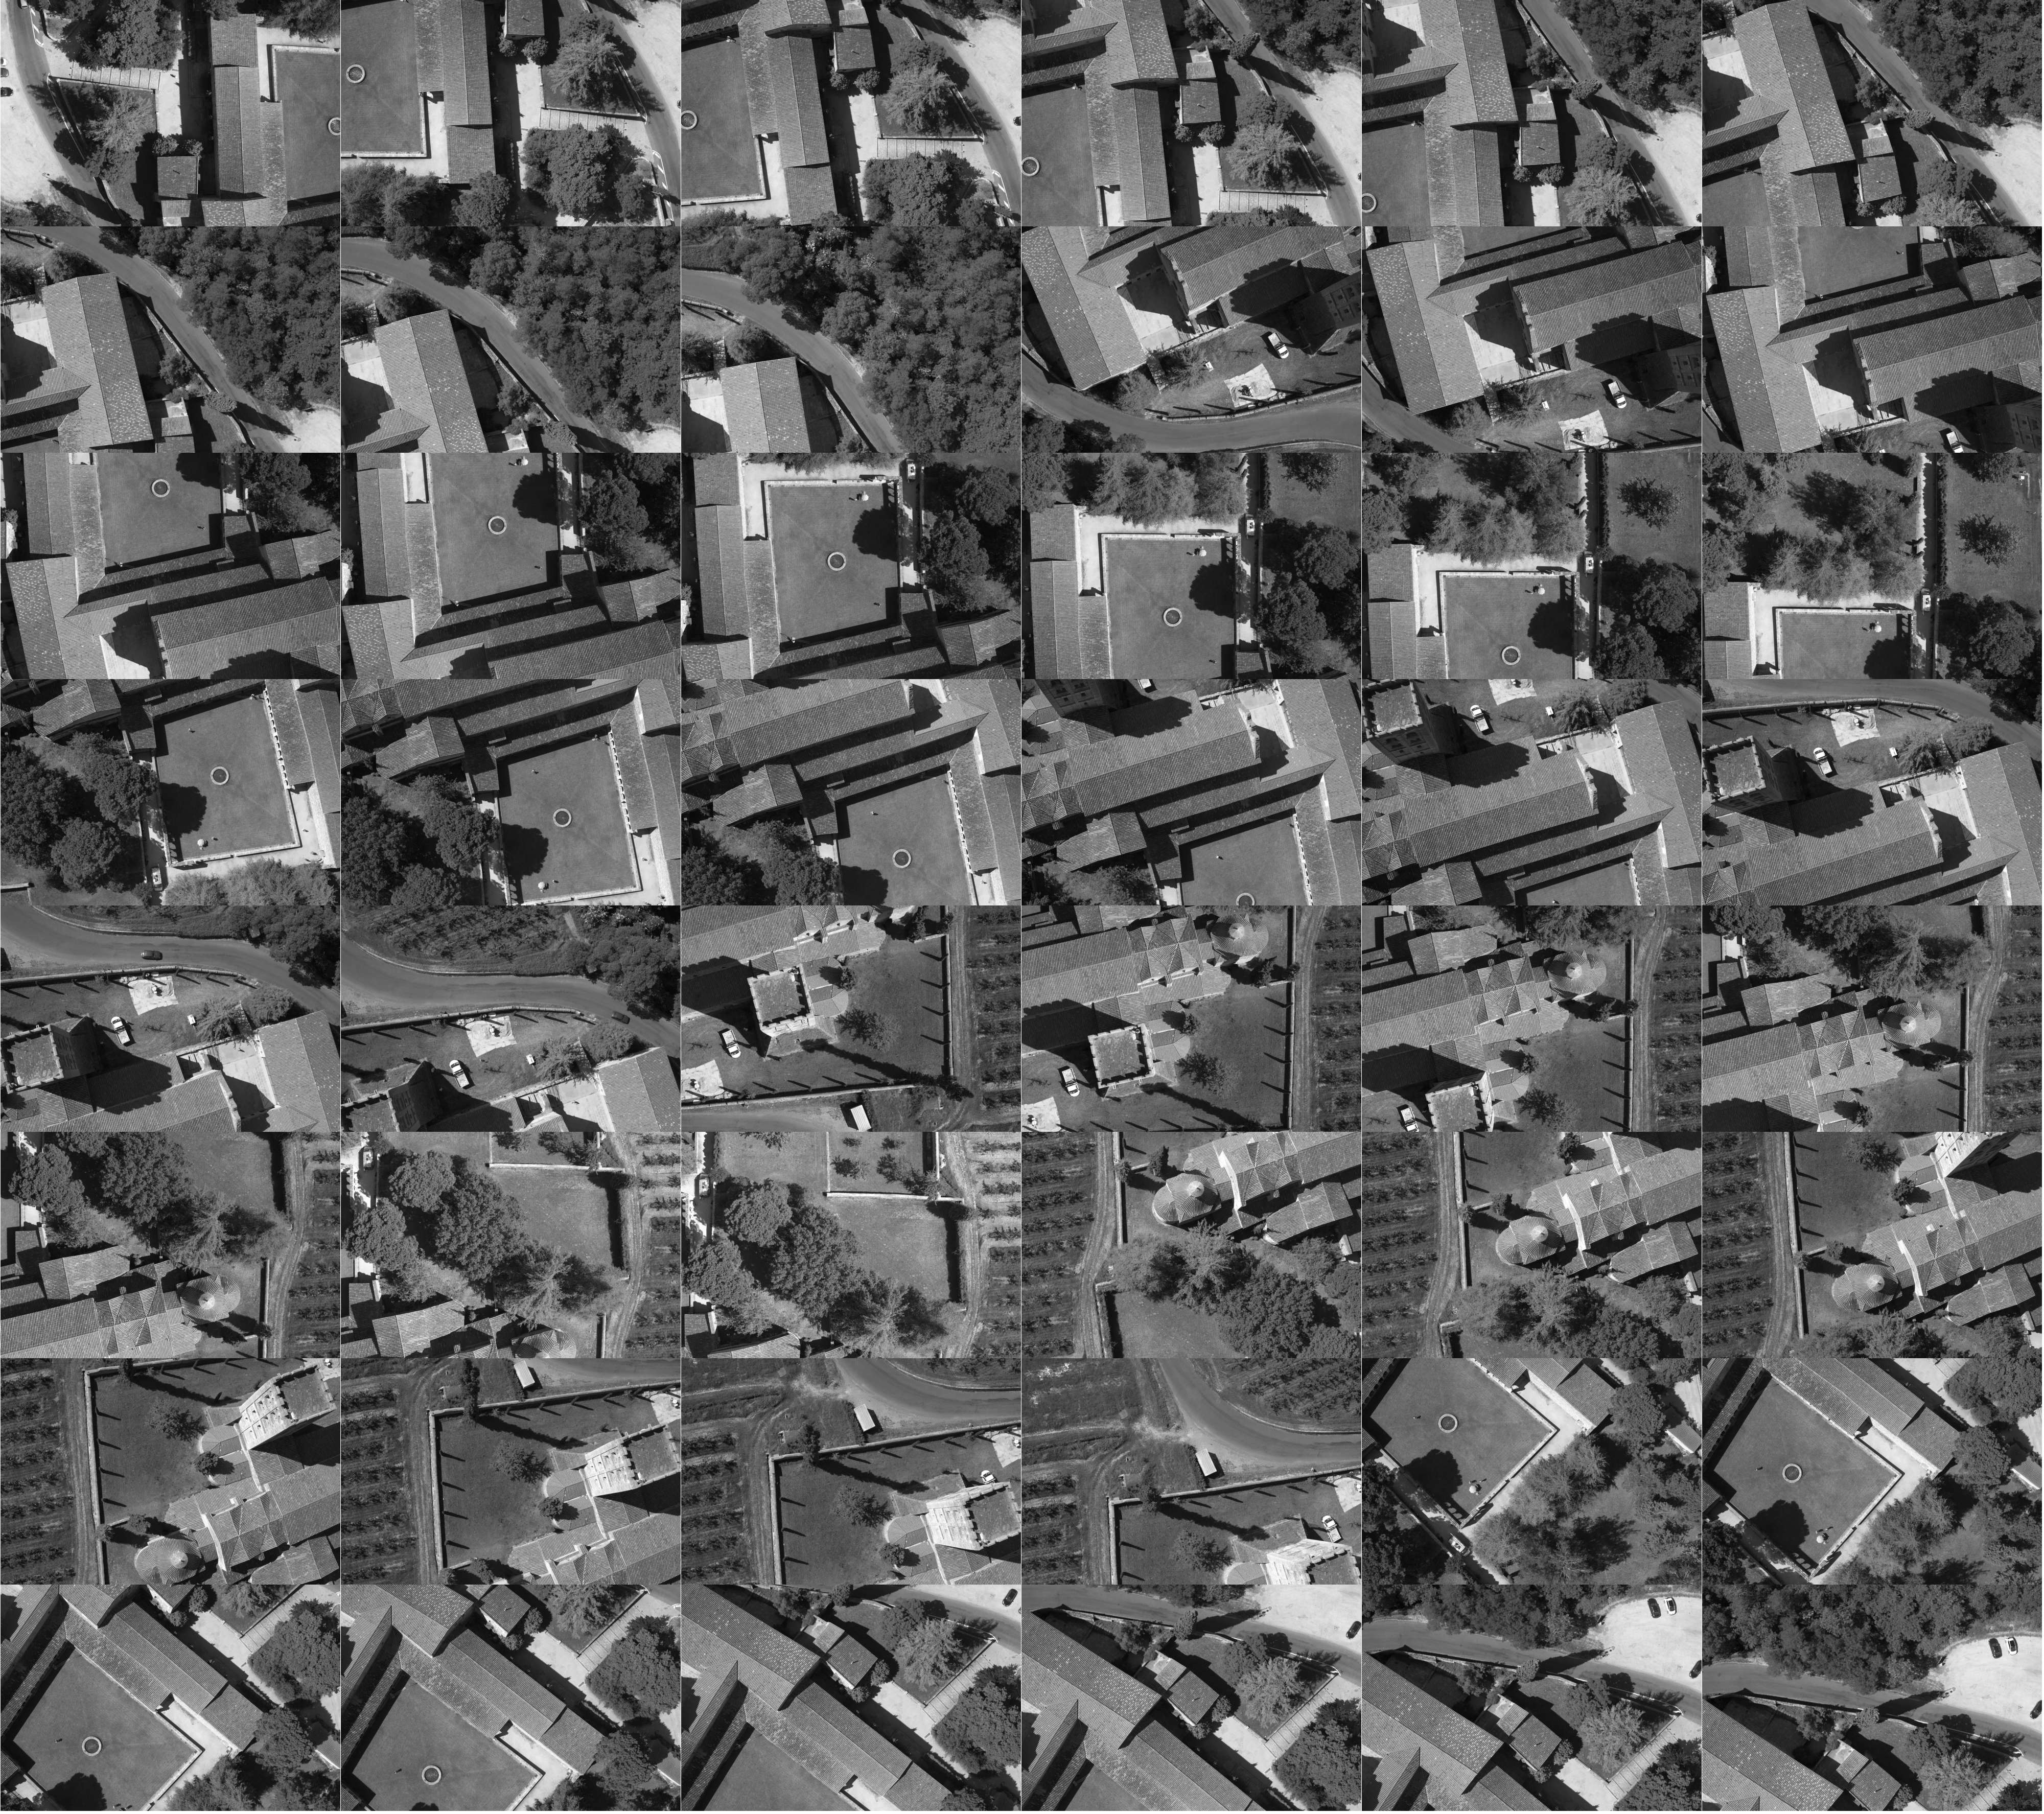
\includegraphics[width=160mm]{FIGS/Cuxa/Planche.jpg}
\caption{Image of Saint-Michel de Cuxa's data set }
\end{center}
\label{FIG:Glob:Cuxa}
\end{figure}

These images have been taken with an helicopter drone at an approximate height of 100 meters, in a typical aerial photogrammetric setup.

\vspace{\baselineskip}
The "standard pipeline" to do a bundle adjustment with ground control points with {\tt MicMac} is:
\begin{itemize}
\item compute images relative orientations, with {\tt Tapioca} and {\tt Tapas};
\item transform GCP coordinates into a local euclidean coordinate system, with {\tt GCPConvert};
\item measure image coordinates for a small set of GCP, with {\tt SaisieAppuisInit};
\item transform image relative orientations into the same local coordinate system, with {\tt GCPBascule};
\item measure image coordinates for all GCP, with {\tt SaisieAppuisPredic};
\item transform image relative orientations into the local coordinate system, with {\tt GCPBascule};
\item run the bundle adjustment, with {\tt Campari};
\item transform back relative orientations into an appropriate coordinate system, with {\tt ChgSysCo};
\item compute a rectified image, with {\tt Tarama};
\item make the matching with {\tt Malt};
\item generate the ortho image with {\tt Tawny};
\end{itemize}

\vspace{\baselineskip}
The file {\tt CmdAbbey.txt} contains all the commands needed to process these data.


%-------------------------------------------------------------------

\subsection{Computing tie points and relative orientations}

    %  -  -  -  -  -  -  -  -  -  -  -  -

\subsubsection{Tie points}

As usual, we want to compute matches between all pairs of calibration data set. This is done by:

\begin{verbatim}
Tapioca MulScale "Abbey-IMG_.*.jpg" 200 800
\end{verbatim}

    %  -  -  -  -  -  -  -  -  -  -  -  -

\subsubsection{Relative orientation}

Then we want to make a first calibration with a subset of the whole data, and
use this calibration as an initial value to the global relative orientation of all images. This is done by:

\begin{verbatim}
Tapas RadialBasic "Abbey-IMG_(0248|0247|0249|0238|0239|0240).jpg" Out=Calib
Tapas RadialBasic "Abbey-.*.jpg" InCal=Calib Out=All-Rel
\end{verbatim}

We can verify that relative orientation was successful by checking the ``Residu Liaison Moyens'' (root mean square error) value that should be around 0.5 pixel.
We can also check visually the result of orientation running {\tt AperiCloud}, described in \ref{APERICLOUD}:

\begin{verbatim}
AperiCloud  "Abbey-IMG_[0-9]*.jpg" All-Rel RGB=0
\end{verbatim}

This will generate the AperiCloud.ply file containing tie points and cameras locations. We can see that cameras are on the same plane, and that the relative orientations match the flight
plan:

\begin{figure}[H]
\begin{center}
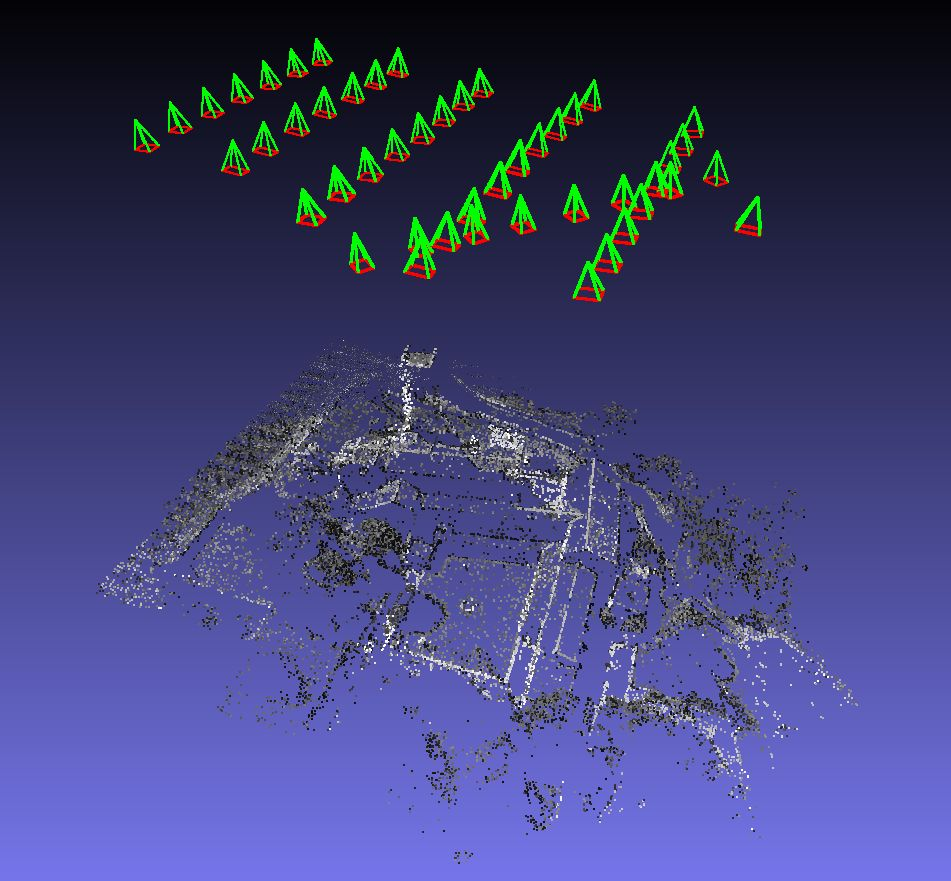
\includegraphics[width=180pt]{FIGS/Cuxa/AperiCloud.jpg}
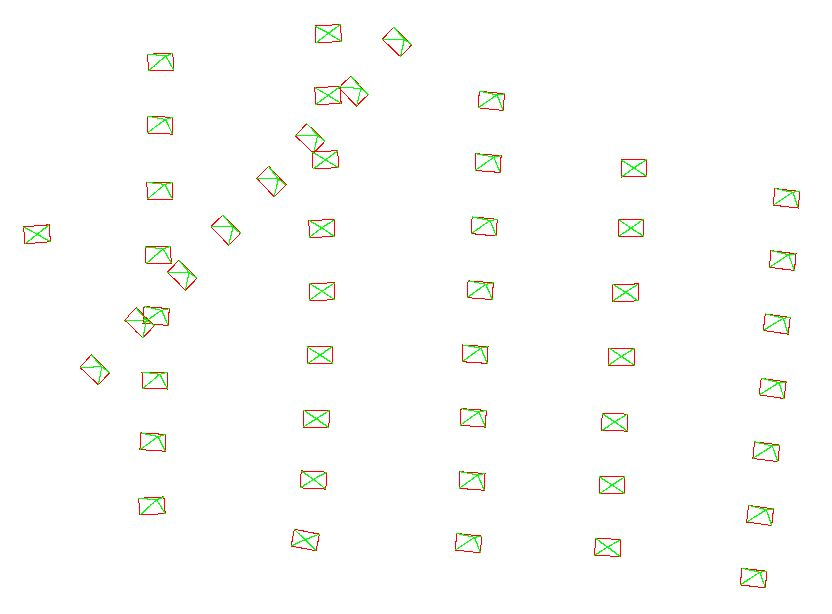
\includegraphics[width=208pt]{FIGS/Cuxa/Aero.jpg}
\caption{Result of relative orientation, computed with {\tt AperiCloud}, perspective and top view.}
\end{center}
\end{figure}

%-------------------------------------------------------------------

\subsection{GCP transforms}

    %  -  -  -  -  -  -  -  -  -  -  -  -

\subsubsection{Ground control point coordinates conversion}

In this use case, we have got ground control points expressed in {\tt WGS84} system. We need to convert them into a local euclidean coordinate system. The important thing is that the local system is euclidean, because all the {\tt MicMac} tools
need this assumption to solve equations. Most of the cartographic coordinate systems are not euclidean systems, so we define a local tangent system, defined around a 3D point and its tangent plane, that will lead to a geometry compliant with {\tt MicMac}'s one.
This is done with the {\tt GCPConvert} tool (detailed in \ref{GCPConvert}):

\begin{verbatim}
GCPConvert "#F=N_X_Y_Z_I" F120601.txt ChSys=DegreeWGS84@SysCoRTL.xml Out=AppRTL.xml
\end{verbatim}

\subsubsection{Ground control point image coordinates input}

To add image coordinates measures, we can use the {\tt SaisieAppuisInit} interface in Linux (detailed in \ref{SaisieAppuisInit}):

\begin{verbatim}
SaisieAppuisInit  "Abbey-IMG_0211.jpg"  All-Rel  NamePointInit.txt  MesureInit.xml
\end{verbatim}

This will create two {\tt Xml} files {\tt MesureInit-S2D.xml} and {\tt MesureInit-S3D.xml}, which respectively contain images coordinates and corresponding 3D coordinates, computed by spatial resection.

\subsubsection{Bascule}

Now we can transform images relative orientations, as computed with Tapas, expressed in an arbitrary coordinate system,
into the local euclidean coordinate system, using 2D images coordinates measures and 3D corresponding ground control points.

\begin{verbatim}
GCPBascule "Abbey-.*jpg" All-Rel  RTL-Init  AppRTL.xml  MesureInit-S2D.xml
\end{verbatim}

Once the images relative orientations have been transformed back in local euclidean coordinate system, one can verify that Z coordinates for the whole data set is nearly constant, which corresponds to the data acquisition setup.

\vspace{\baselineskip}
Possible error: "{\tt Not enough samples (Min 3) in cRansacBasculementRigide}". It means that there is not enough points to compute a Bascule transform. You should add more points with {\tt SaisieAppuisInit}:
at least 3 GCP whose projection are known in at least 2 images are needed.

\subsubsection{Adding points with predictive interface {\tt SaisieAppuisPredic}}

When the global transform between ground control points and image relative orientations is known, we can switch to the predictive interface {\tt SaisieAppuisPredic} which will display the remaining ground control points, loaded from the {\tt Xml} file {\tt AppRTL.xml}.
You need to adjust points image location and validate them.

\begin{verbatim}
SaisieAppuisPredic  "Abbey-.*jpg" RTL-Init AppRTL.xml  MesureFinale.xml
\end{verbatim}

\subsubsection{Bascule}

Again we can transform images relative orientations, this time with a more substantial number of images measures, which will give a better transform.
\begin{verbatim}
GCPBascule "Abbey.*jpg" All-Rel  RTL-Bascule AppRTL.xml MesureFinale-S2D.xml
\end{verbatim}

%-------------------------------------------------------------------

\subsection{Bundle adjustment with ground control points}

\label{Bundle:CAMPARI}

Now we can run a constrained bundle adjustment combining ground control points and tie points, with the {\tt Campari} command, described in \ref{CAMPARI}.

\begin{verbatim}
Campari "Abbey.*.jpg"  RTL-Bascule RTL-Compense GCP=[AppRTL.xml,0.1,MesureFinale-S2D.xml,0.5]
\end{verbatim}

%-------------------------------------------------------------------

\subsection{Post-processing}

\subsubsection{Coordinate system backward transform}

Then one can transform coordinates from the local euclidean coordinate system to a geographic coordinate system, and compute ortho-images which can be superimposed on vectorial maps (and \textit{vice versa}).
For example, if we want to transform our data into the sinusoidal projection, for which we have got a file {\tt SysCoSinus90W.xml} storing the transformation parameters, the command is:

\begin{verbatim}
ChgSysCo  "Abbey.*.jpg" RTL-Compense SysCoRTL.xml@SysCoSinus90W.xml Sin90

Tarama  "Abbey.*.jpg" Sin90

Malt Ortho  "Abbey.*.jpg" Sin90 SzW=1 AffineLast=false DefCor=0.0

Tawny Ortho-MEC-Malt/
\end{verbatim}

\begin{figure}[H]
\begin{center}
\includegraphics[width=150mm]{FIGS/Cuxa/Sinus-Ortho-Eg-Test-Redr.jpg}
\caption{Image rectification in sinusoidal projection, with {\tt Tarama}}
\end{center}
\end{figure}

%\begin{figure}[H]
%\begin{center}
%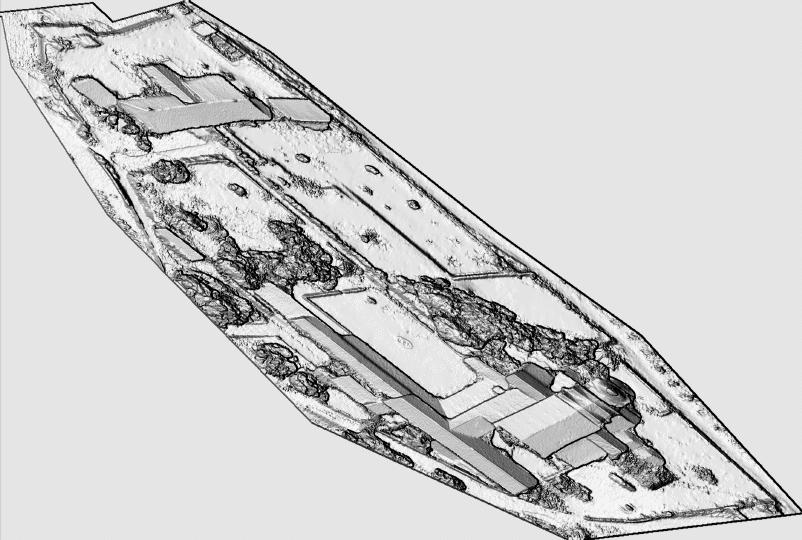
\includegraphics[width=150mm]{FIGS/Cuxa/SinusShade.jpg}
%\caption{Shading in sinusoidal projection, with {\tt GrShade}}
%\end{center}
%\end{figure}

The result is ugly, but if we have a look to the global earth mapping with sinusoidal projection, it is obvious that we cannot have a good representation at the European longitude with the sinusoidal projection.

\begin{figure}[H]
\begin{center}
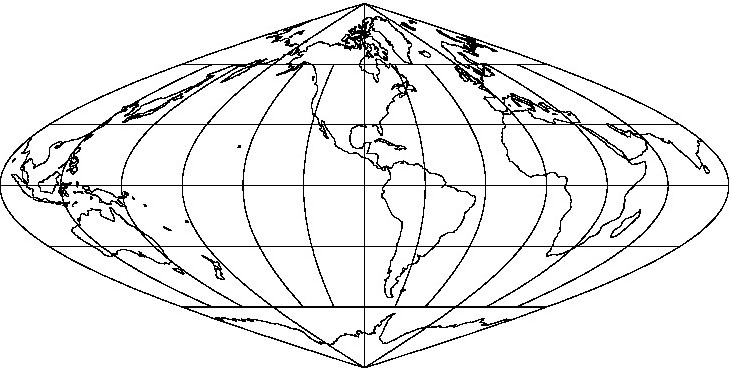
\includegraphics[width=182pt]{FIGS/Cuxa/Sinus90.jpg}
\caption{Sinusoidal projection, with Central Meridian $90\,^{\circ}$W}
\end{center}
\end{figure}

What we expect would be more like the result of a projection in Lambert93 coordinate system:

\begin{verbatim}
ChgSysCo  "Abbey.*.jpg" RTL-Compense SysCoRTL.xml@Lambert93 L93

Tarama  "Abbey.*.jpg" L93

Malt Ortho  "Abbey.*.jpg" L93 SzW=1 AffineLast=false DefCor=0.0

Tawny Ortho-MEC-Malt/
\end{verbatim}

\begin{figure}[H]
\begin{center}
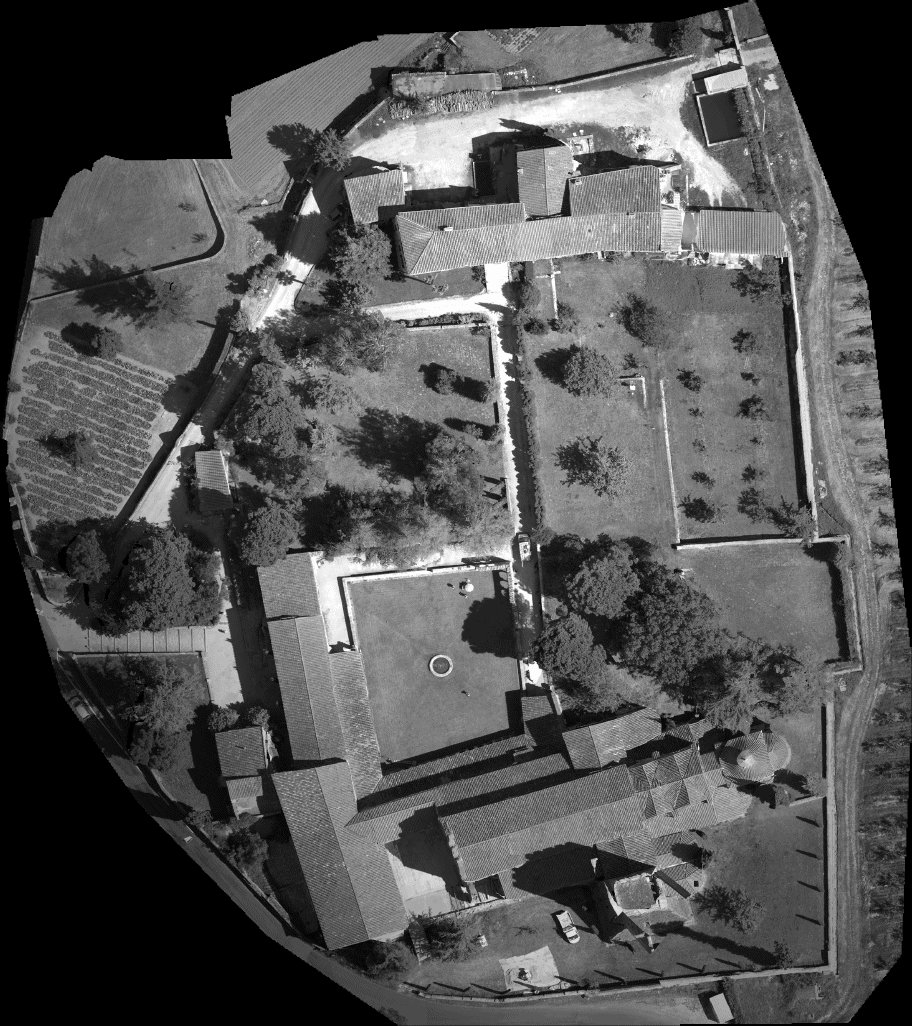
\includegraphics[width=160mm]{FIGS/Cuxa/L93-Ortho-Eg-Test-Redr.jpg}
\caption{Image rectification in Lambert93 projection, with {\tt Tawny}}
\end{center}
\end{figure}

\begin{figure}
\begin{center}
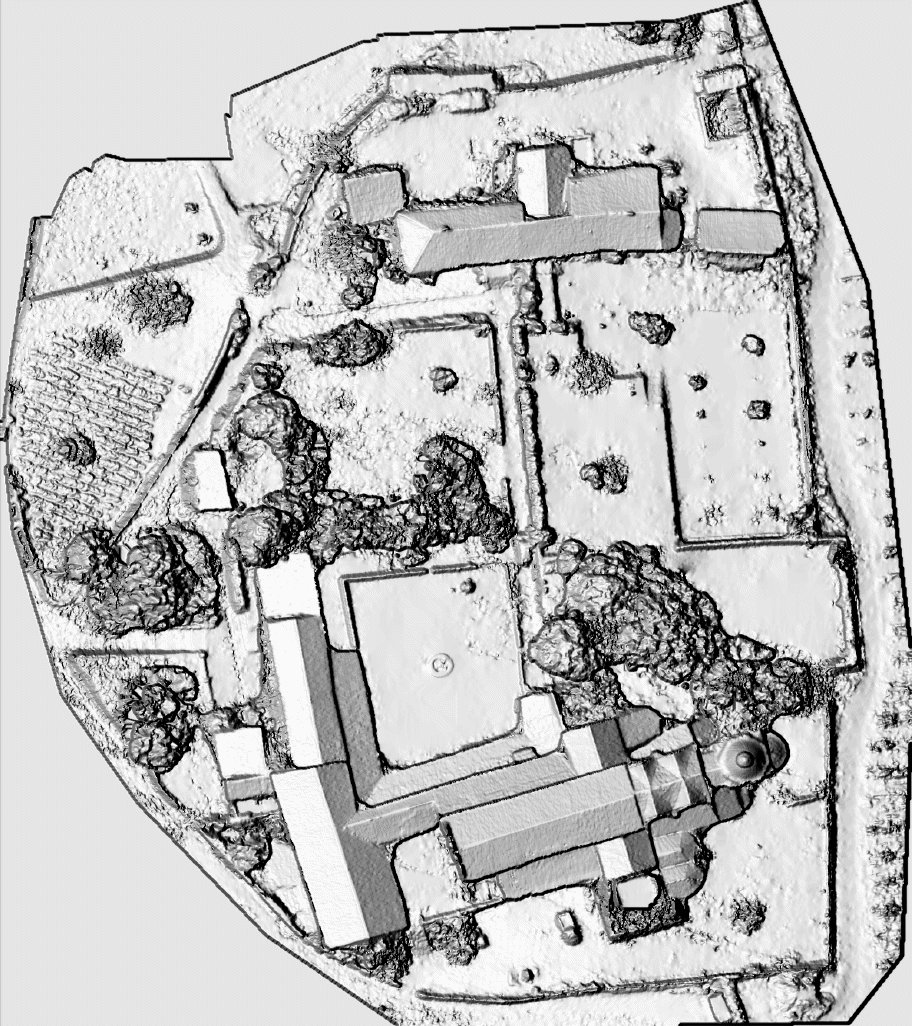
\includegraphics[width=160mm]{FIGS/Cuxa/L93-Shade.jpg}
\caption{Shading in Lambert93 projection, with {\tt GrShade}}
\end{center}
\end{figure}

%-------------------------------------------------------------------
\section{The Grand-Leez dataset}
%-------------------------------------------------------------------

\subsection{Dataset description}\label{Grand-Leez:DataSet}

The directory {\tt UASGrandLeez/} in {\tt micmac\_data/ExempleDoc/}, contains UAS\footnote{Unmanned Aerial System or {\tt drone}} imagery which are used to illustrate a complete workflow devoted to the the production of a canopy surface model. 
The aerial survey was performed by the lab of Forest and Nature Management\footnote{\url{http://www.gembloux.ulg.ac.be/gestion-des-ressources-forestieres-et-des-milieux-naturels/}} of the University of Liege (Belgium). 
The image block is made up of 200 low-oblique vantage jpeg images, acquired with a Ricoh GRIII (10 Mpixels, focal length of 28 mm 35 equivalent). 
The flight was performed with a Gatewing X100 platform.
The inertial measurement unit provides GPS position and attitude (omega, phi, kappa) of the UAS for each image frame (stored in {\tt GPS\_WPK\_Grand-Leez.csv} file). 
In order to reduce the size of this dataset, raw images were resampled to 800 pixels width. 
The processing of these images can however take a few hours. 
The file {\tt  Documentation/FIGS/UASGrandLeez/Cmd\_UAS\_Grand-Leez.txt} contains all the command lines related to this processing workflow.

First, let's take a look at the images. 
A convenient tool to visualize multiple images in a panel is the {\tt PanelIm} tool which was used to produce figure \ref{FIG:panel-GL} and other image panels in this manual:

\begin{figure}[H]
\centering
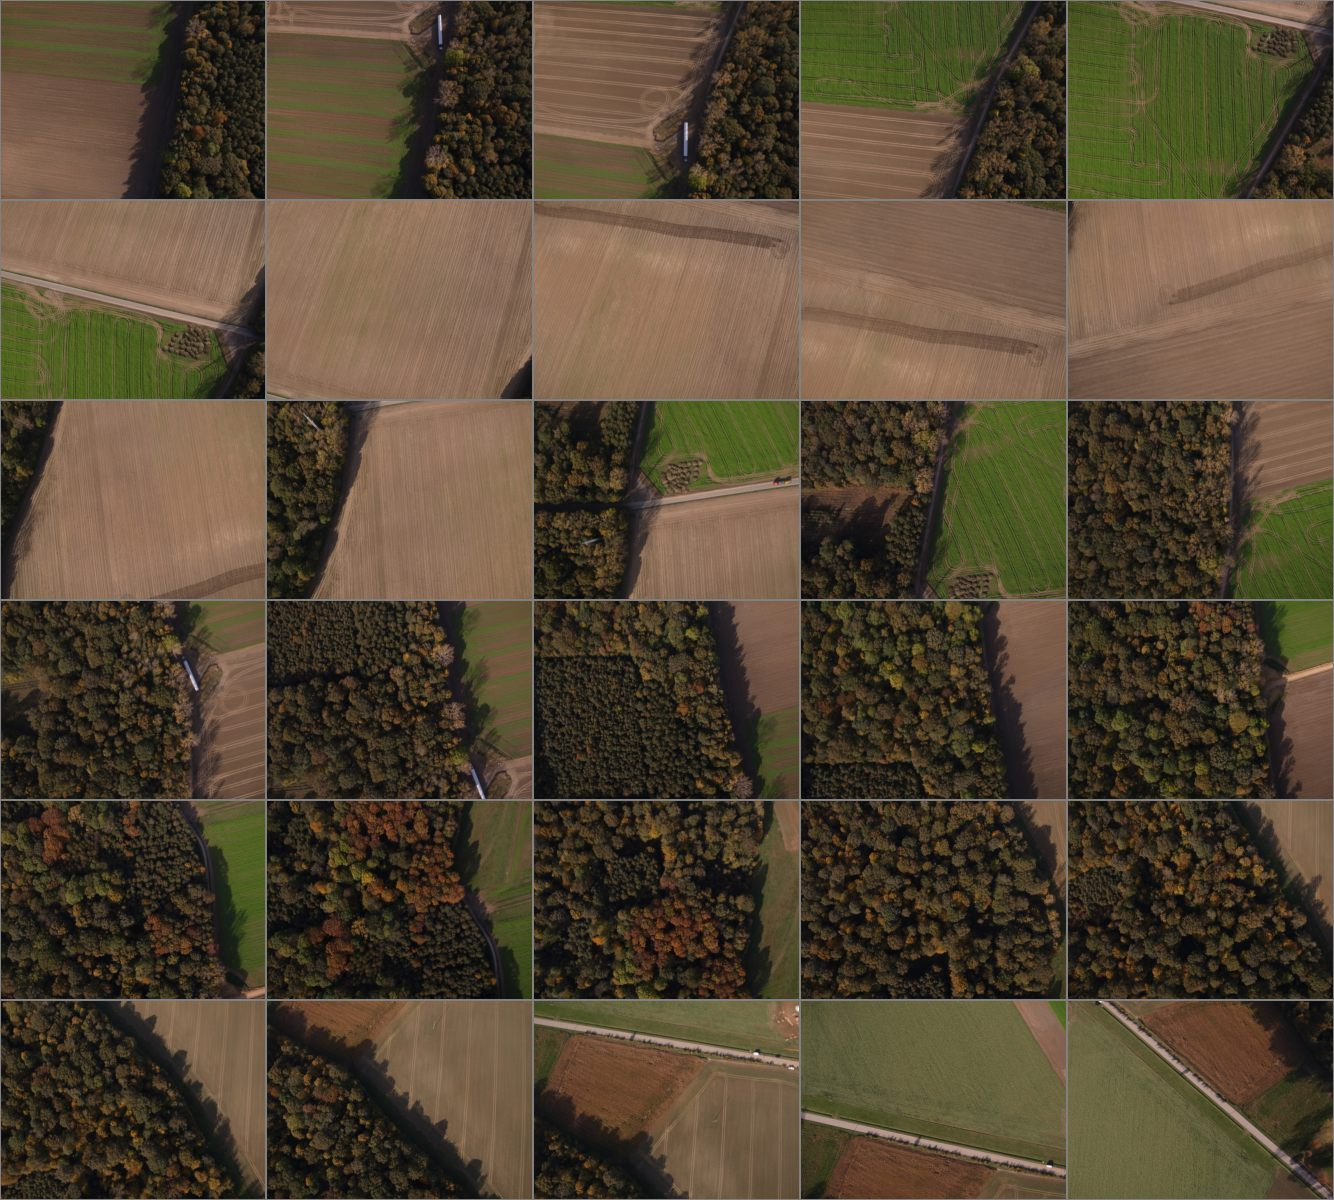
\includegraphics[height=0.5\linewidth]{FIGS/UASGrandLeez/PanelGL.JPG}
\caption{The Grand-Leez dataset}
\label{FIG:panel-GL}
\end{figure}

\begin{verbatim}
mm3d PanelIm ./ "R00405[0-5][0:2:4:6:8].JPG" Scale=3
\end{verbatim}

In this example, we deal with direct georeferencing, which consist of using camera positions (or camera center) to georeference the photogrammetric model. 
At first, the tool {\tt OriConvert} (section \ref{OriConvert})  is used to convert telemetry data into {\tt MicMac} format. 
Telemetry data aren't exclusively used for georeferencing, but also to determine potential image pairs.
The list of image pairs is then used for the computation of tie points ({\tt Tapioca File \dots}). 
In addition, embedded GPS data are used in a constrained bundle block adjustment in order to avoid non-linear distortions which can hinder photogrammetric measurements.

The pipeline presented here to process UAS imagery with embedded GPS data with {\tt MicMac} is organized as follows:
\vspace{\baselineskip}
\begin{enumerate}
 \setlength{\itemsep}{0pt}
  \setlength{\parskip}{0pt}
\item Transform initial external orientation file (embedded GPS data) into the {\tt MicMac} format and generate an image pairs file with {\tt OriConvert}. 
In addition, latitude and longitude GPS information are projected in the Belgian Lambert 72 coordinate system;
\item Compute image tie points with {\tt Tapioca File};
\item Initialize the image block orientation with {\tt Martini};
\item Determine image relative orientation, with {\tt Tapas};
\item Transform image relative orientation into absolute orientation, e.g. performing direct georeferencing, with {\tt CenterBascule};
\item Improve the aerotriangulated model by adding GPS information in the bundle block adjustment, with {\tt Campari};
\end{enumerate}
\vspace{-0.8\topsep}
It results in the image orientation ({\tt Ori-BL72-Campari}), which is used to perform the image dense matching and subsequently the image orthorectification and mosaicking.
The canopy surface is characterized by many abrupt vertical changes, which are difficult to model by image matching. 
The dense matching is performed in \textit{image geometry} with the \textit{Per Image Matchings} tool {\tt PIMs}. 
Thus, one depth map is computed for each image. 
These depth maps are then georeferenced and merged in one single digital surface model covering the entire area.
The canopy surface model is then used of orthorectification and individual orthoimages are then mosaicked.
The remaining of the workflow is thus as follows;
\vspace{-0.8\topsep}
\begin{enumerate}\addtocounter{enumi}{6}
 \setlength{\itemsep}{0pt}
  \setlength{\parskip}{0pt}
\item Compute depth map for each image with \textit{Per Image Matching} Tools ({\tt PIMs});
\item Merge individual depth maps in a global Digital Surface Model  and compute orthoimage with {\tt PIMs2Mnt};
\item Merge individual orthoimages in an orthophotomosaic with {\tt Tawny}.
\end{enumerate}
\vspace{-0.8\topsep}

\subsection{Computing tie points and absolute orientation}

Figure \ref{FIG:workflowGLOri} illustrates the determination of the orientation for the image block.
The final orientation database which is used for the dense matching process and for orthophoto generation is the folder \textit{Ori-BL72-Campari}.

\begin{figure}[H]
\centering
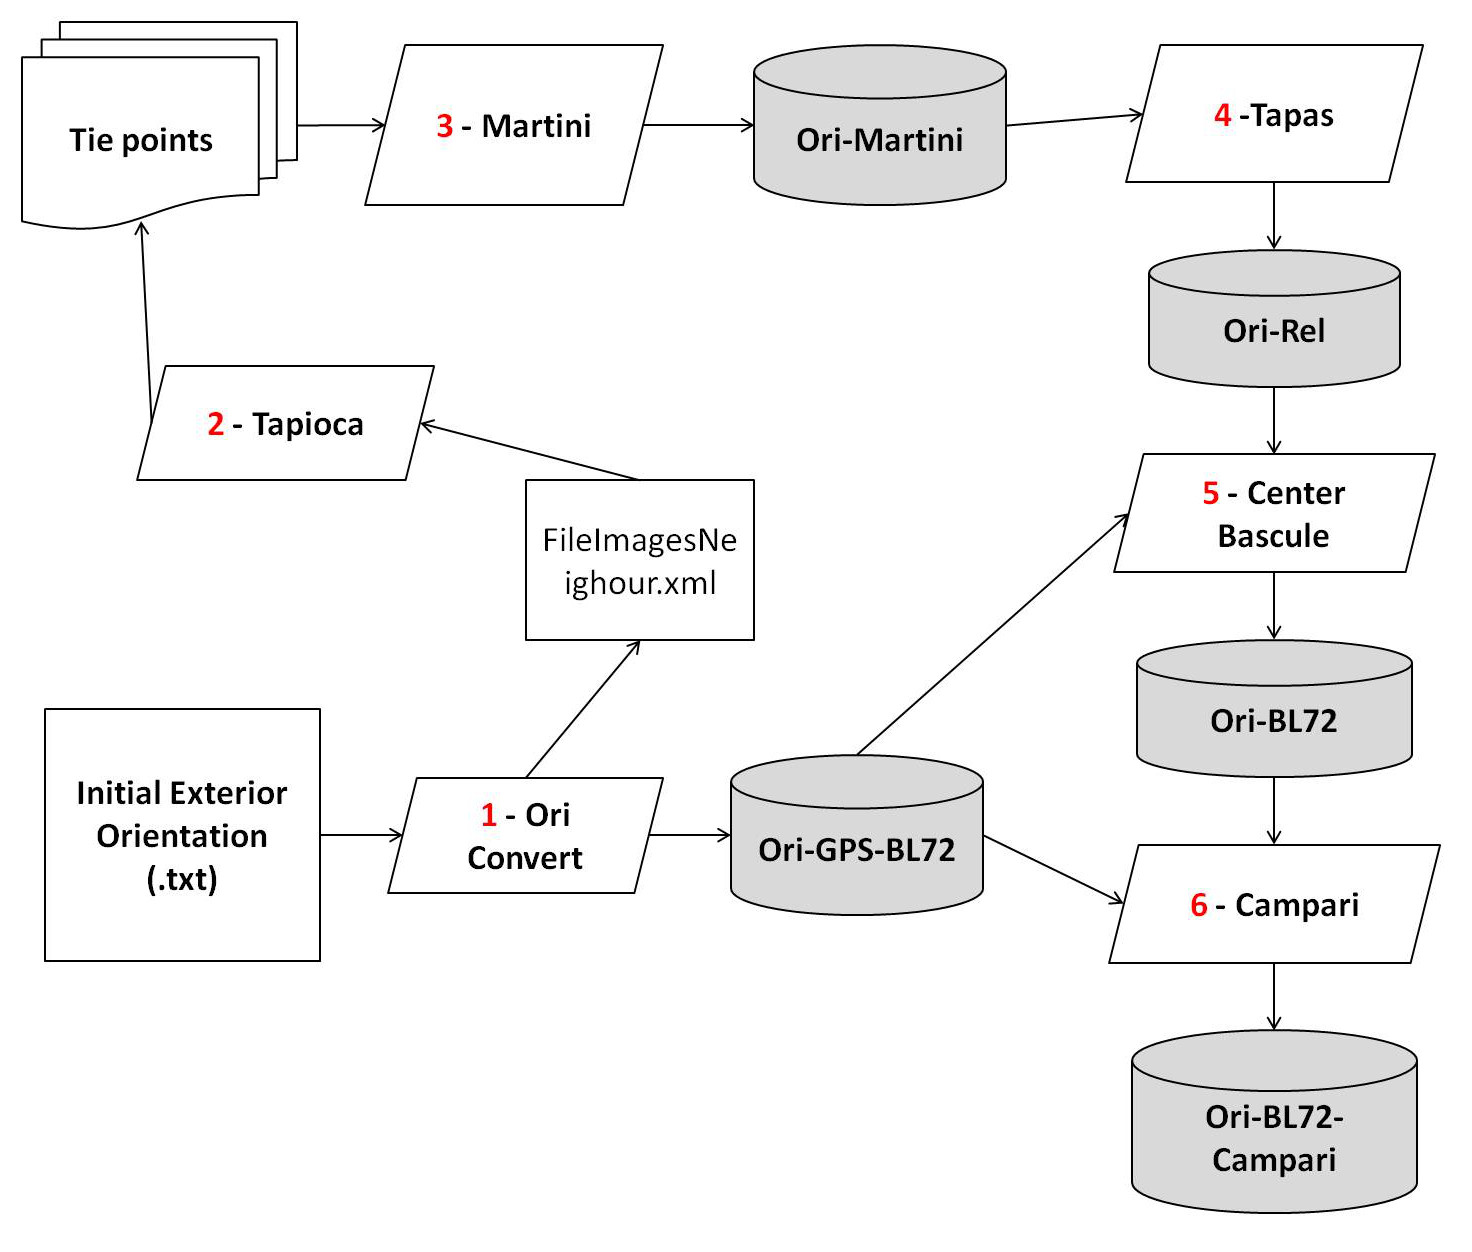
\includegraphics[width=0.9\linewidth]{FIGS/UASGrandLeez/workflowGLOri.jpg}
\caption{The processing chain for computing the image orientation (\textit{Ori-BL72-Campari}). Processing steps are numbered in red.}
\label{FIG:workflowGLOri}
\end{figure}

\subsubsection{Conversion of GPS data in {\tt MicMac} format}

\begin{verbatim}
mm3d OriConvert OriTxtInFile GPS_WPK_Grand-Leez.csv GPS-BL72  MTD1=1\
       ChSys=DegreeWGS84@SysCoBL72_EPSG31370.xml  NameCple=FileImagePairs.xml 
\end{verbatim}
Note that {\tt MicMac} uses the proj4 library to change the coordinate systems. 
The Belgian Lambert 72 coordinate system is defined using its "proj4 code" written in an xml file (see {\tt SysCoBL72\_EPSG31370.xml})

\subsubsection{Tie points}
The file {\tt FileImagePairs.xml} is used for computing tie points with {\tt Tapioca}.

\begin{verbatim}
Tapioca File ``FileImagePairs.xml'' -1
\end{verbatim}

Tie points are used as observations in the bundle adjustment ({\tt Tapas} and {\tt Campari}) to determine the element of image orientation (external orientation and camera calibration). 

\subsubsection{Relative orientation}

Initialization of the orientation for a large image block (hundreds of image) can be carried out with the {\tt Martini} tool:

\begin{verbatim}
mm3d Martini "R.*.JPG"
AperiCloud "R.*.JPG" Martini Out=Martini-cam.ply WithPoints=0
\end{verbatim}
As {\tt Martini} does not account for any radial distortion of the lens, the visual inspection of the image orientation with {\tt AperiCloud} shows large non-linear distortions.
Initialization of the image orientation can also be performed successfully directly with {Tapas}, but for a large image block, the use of {\tt Martini} is faster.
The complete dataset is then aligned in a relative orientation {\tt Rel} with the following command line:

\begin{verbatim}
Tapas RadialBasic "R.*.JPG" Out=Rel InOri=Martini
\end{verbatim}

\subsubsection{Georeferencing}

The center database {\tt Ori-GPS-BL72} is employed to georeference the aerotriangulated model with { \tt CenterBascule}:

\begin{verbatim}
CenterBascule "R.*.JPG" Rel GPS-BL72 BL72
\end{verbatim}

\subsubsection{Bundle adjustment with embedded GPS data}

Adding GPS information in the bundle adjustment has a positive impact on the refinement of the camera orientation, in particular on the camera calibration.
\begin{verbatim}
Campari "R.*.JPG" BL72 BL72-Campari EmGPS=[GPS-BL72,2] FocFree=1 PPFree=1
\end{verbatim}

\subsection{Dense matching and orthorectification}

The digital surface model of the canopy is created with {\tt PIMs} and {\tt PIMs2Mnt}.

\begin{verbatim}
mm3d PIMs Forest "R00.*.JPG" BL72-Campari  ZoomF=2
\end{verbatim}

The mode {\tt Forest} of the {\tt PIMs} tool is appropriate for aerial images of forested zones. 
In this mode, a dense matching is performed independently for every pair of successive images.
In the terminal, a message display the pairs that will be used for stereo image matching (in epipolar geometry):
\begin{verbatim}
Adding the following image pair: R0040571.JPG and R0040570.JPG 
Adding the following image pair: R0040572.JPG and R0040571.JPG 
Adding the following image pair: R0040573.JPG and R0040572.JPG 
...
\end{verbatim}

Dense matching is time consuming and generates a lot of intermediate results.
Figure \ref{FIG:pimsGL} illustrates the functioning of the  \textit{Per Image Matchings} approach.

\begin{figure}
\centering
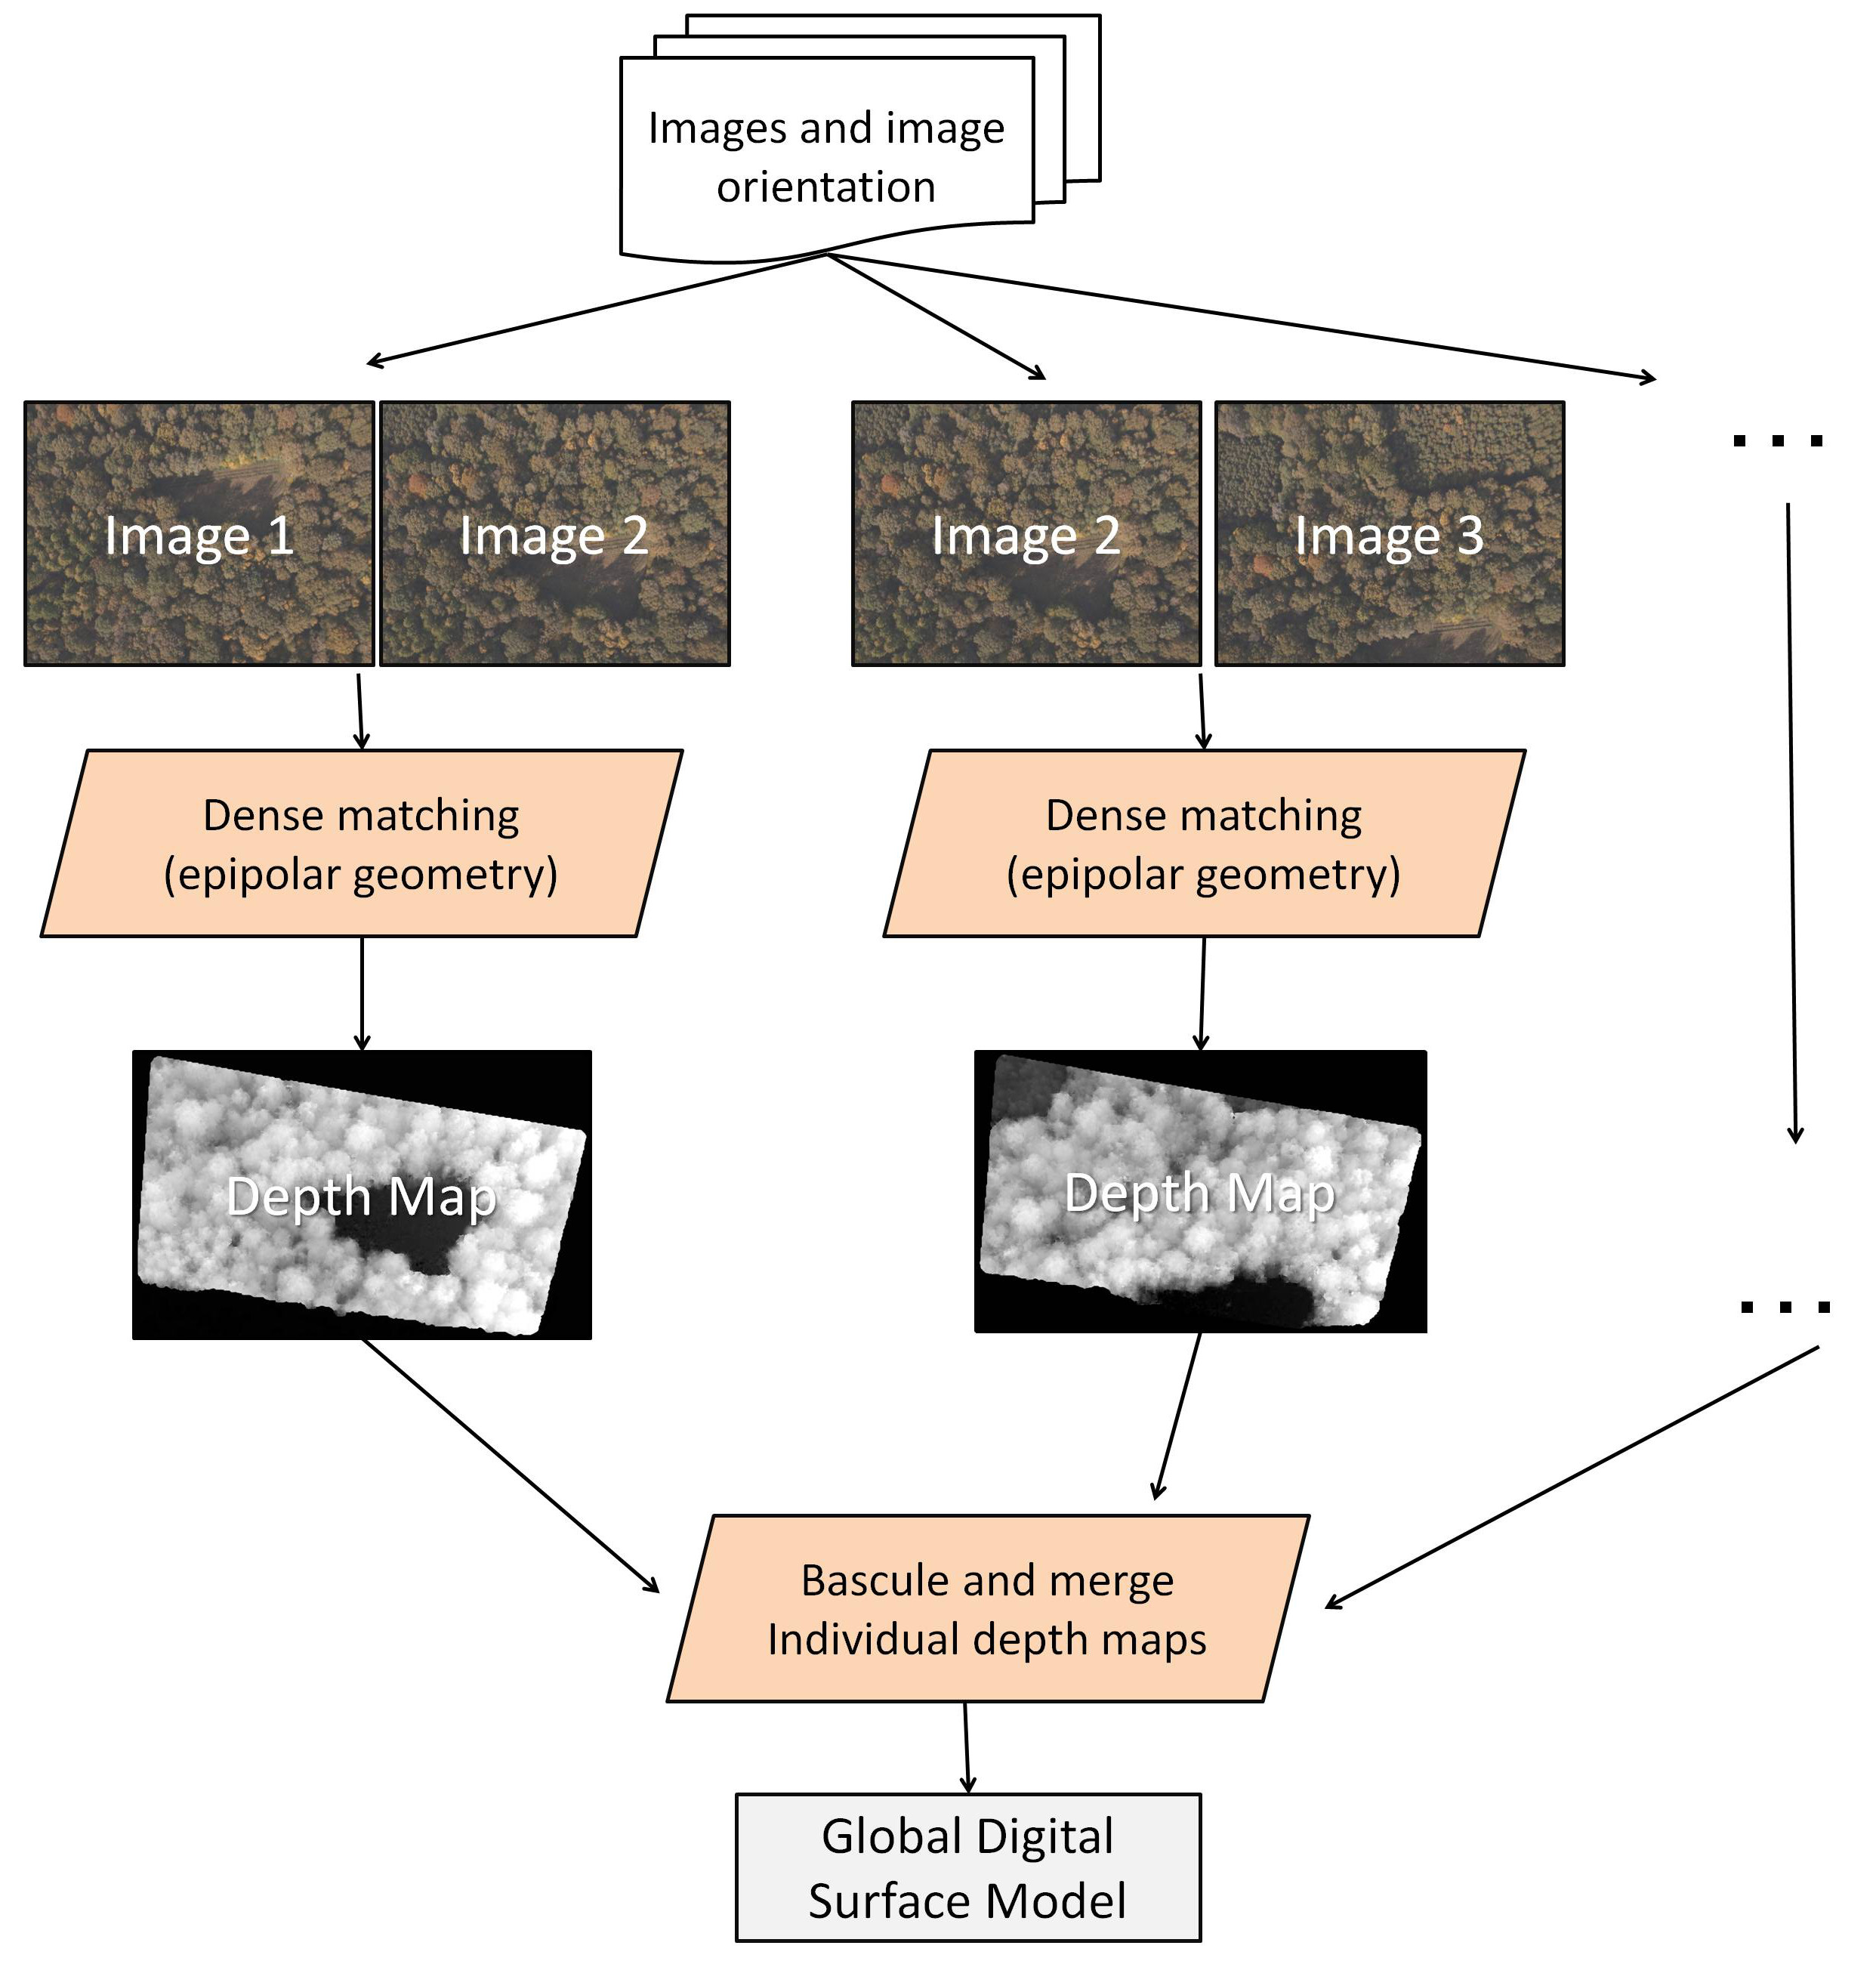
\includegraphics[width=0.8\linewidth]{FIGS/UASGrandLeez/PIMsGL.jpg}
\caption{Simplified representation of the functioning of the \textit{Per Image Matchings} approach implemented in the {\tt PIMs Forest} tool.
Image dense matching is performed for a list of image pairs, resulting in one (or more) depth map per image.
These depth maps are georeferenced and merged together with the tools {\tt PIMs2Mnt}. }
\label{FIG:pimsGL}
\end{figure}

Stereo depth maps are merged together with {\tt PIM2Mnt}. 
Subsequently, orthorectification is performed for each image and orthoimages are stored in the directory { \tt PIMs-ORTHO/}.

\begin{verbatim}
mm3d PIMs2Mnt Forest DoOrtho=1
\end{verbatim}

The global digital surface model resulting from the merging of every single depth map is the raster file named {\tt PIMs-TmpBasc/PIMs-Merged\_Prof.tif}.
It can be visualized and analysed in any GIS software. 
Eventually, orthoimages are mosaicked together with {\tt Tawny}.
Because the radiometry of the different images are quite similar (no important illumination changes during the image acquisition), no radiometric equalization is performed ({\tt RadiomEgal=0}).

\begin{verbatim}
Tawny PIMs-ORTHO/ RadiomEgal=0 Out=Orthophotomosaic.tif
\end{verbatim}

The digital surface model and the orthophotomosaic can be combined in a colored 3D point cloud with  {\tt Nuage2Ply } (see figure \ref{fig:GL_nuage}).

\begin{verbatim}

# export the dense point cloud and colorize it with Nuage2Ply:
Nuage2Ply "PIMs-TmpBasc/PIMs-Merged.xml" Scale=1 /
	Attr="PIMs-Ortho/Orthophotomosaic.tif" RatioAttrCarte=2 Out=CanopySurfaceModel.ply
       
# Optionally, if meshlab is installed:
meshlab CanopySurfaceModel.ply
\end{verbatim}

\begin{figure}
\centering
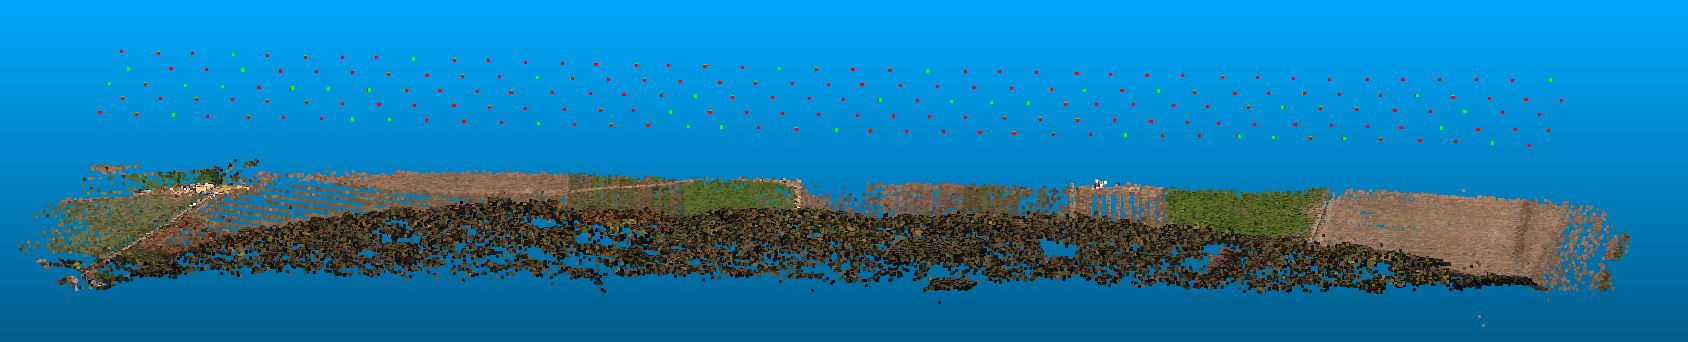
\includegraphics[width=\linewidth]{FIGS/UASGrandLeez/GL_ori.jpg}
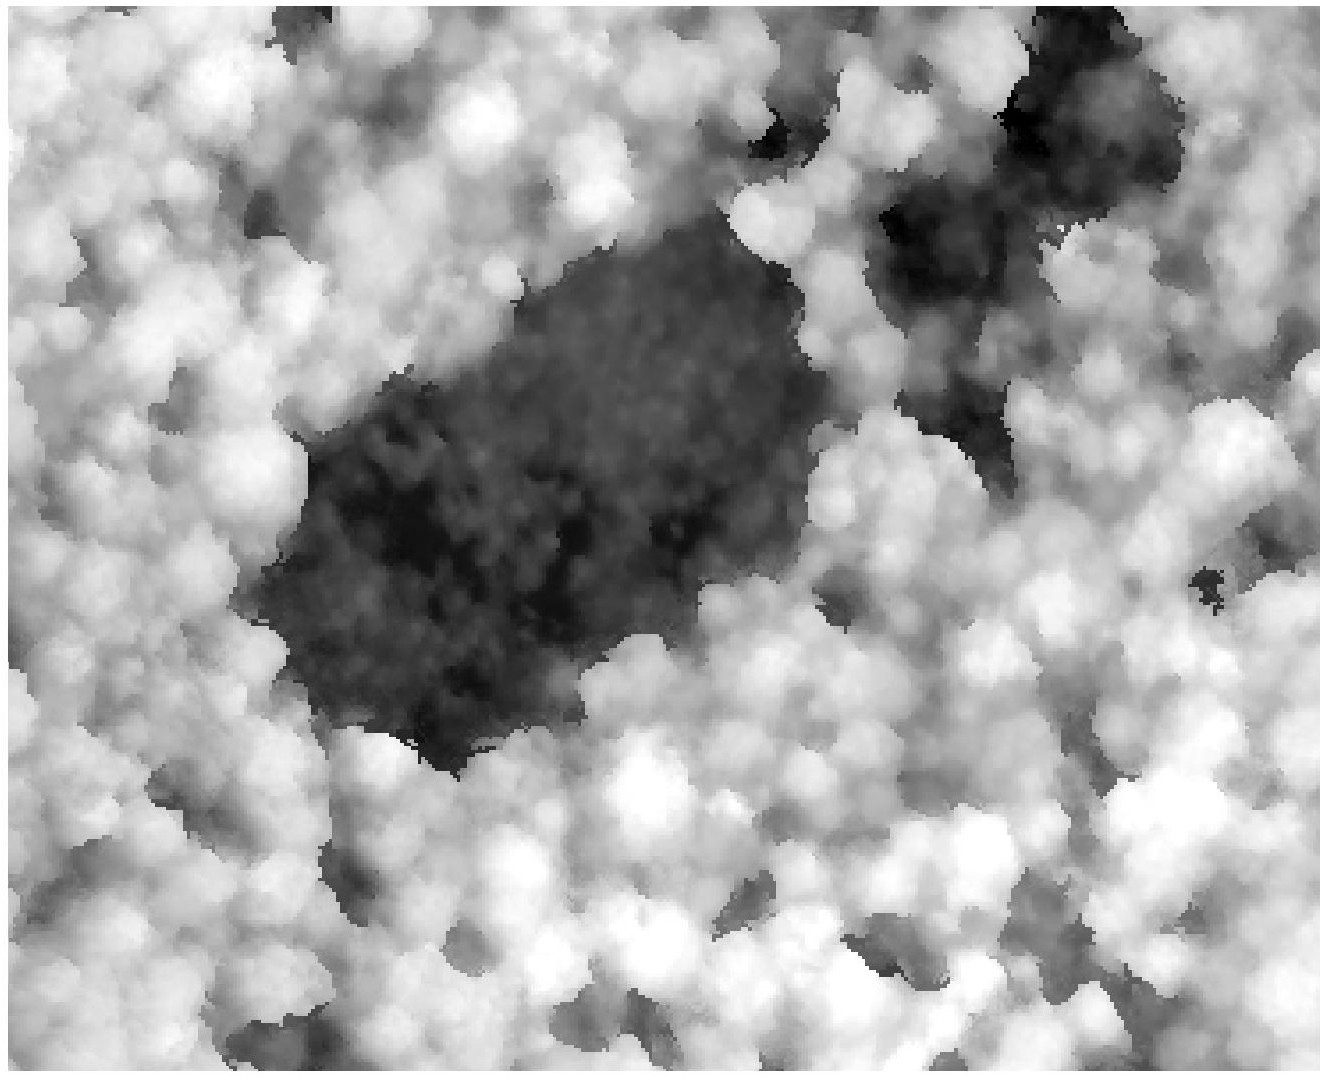
\includegraphics[width=0.49\linewidth]{FIGS/UASGrandLeez/GL_zoomDSM.jpeg}
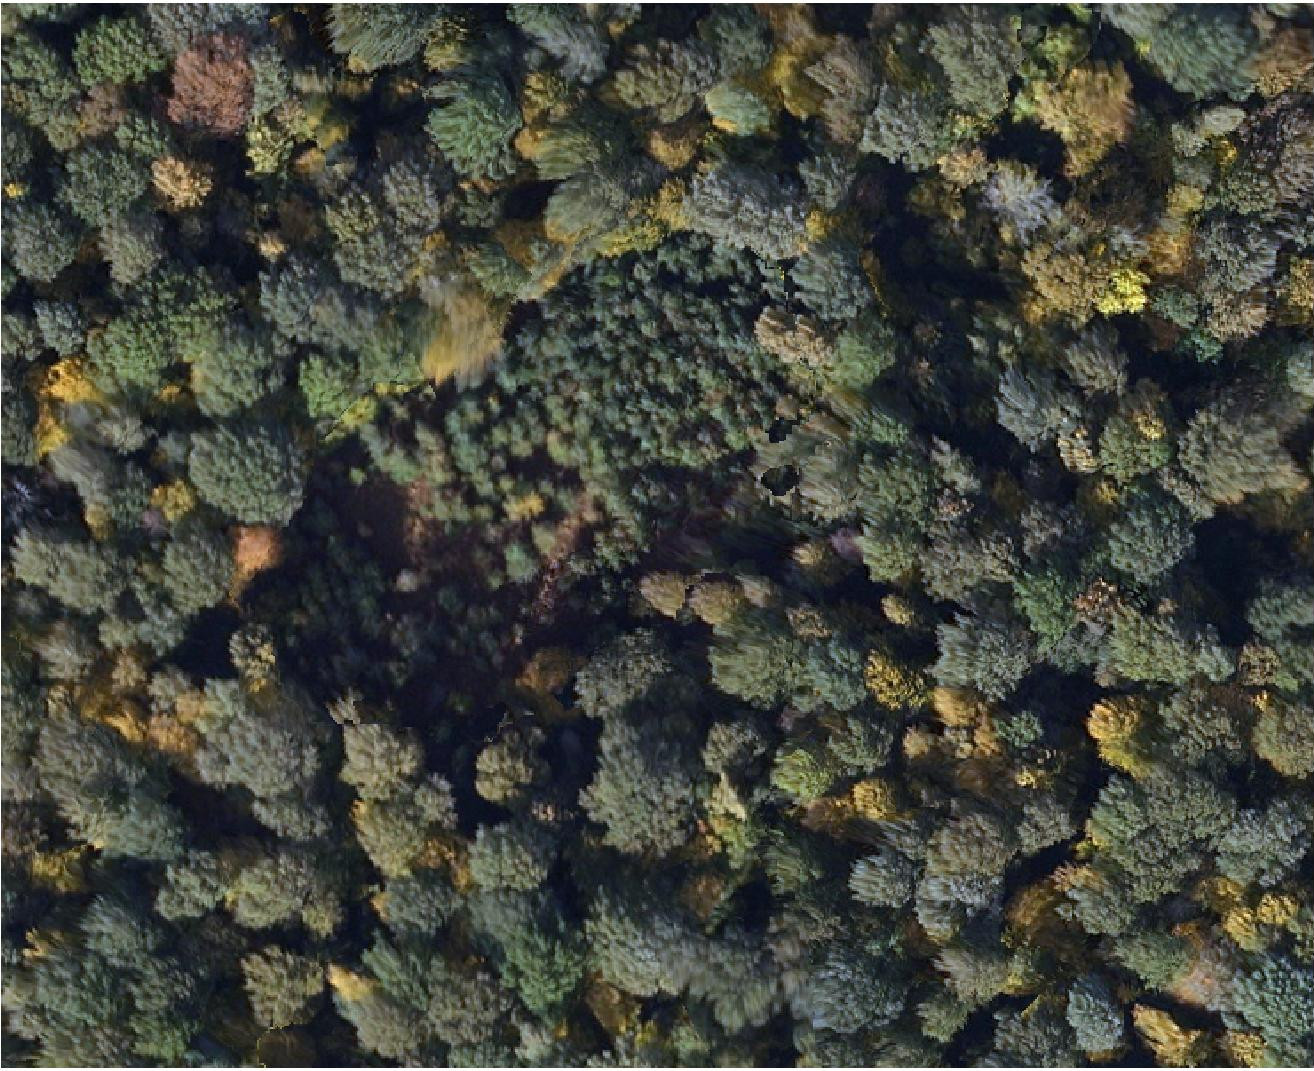
\includegraphics[width=0.49\linewidth]{FIGS/UASGrandLeez/GL_zoomOrtho.jpeg}
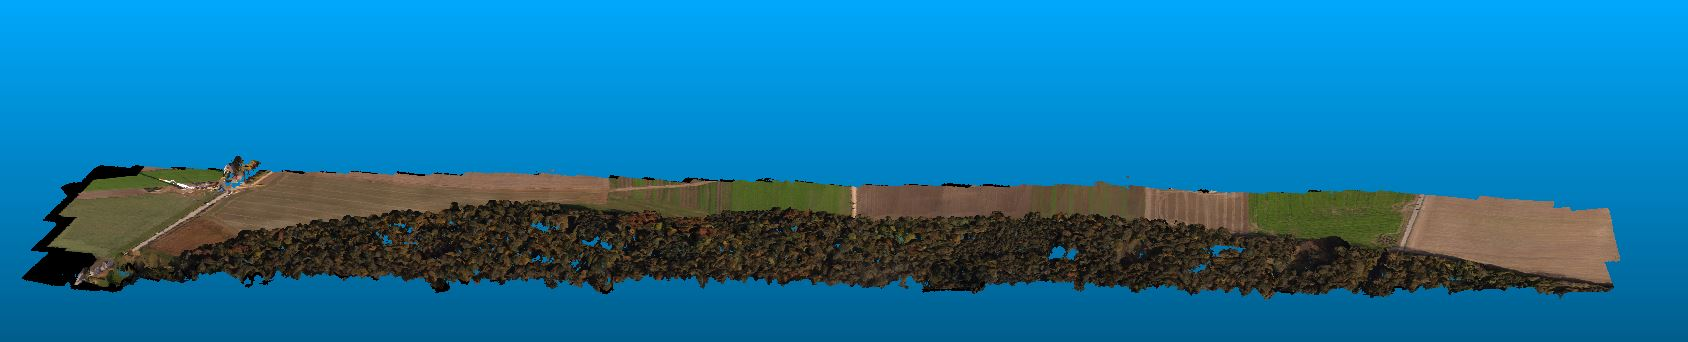
\includegraphics[width=\linewidth]{FIGS/UASGrandLeez/GL_denseCloud.jpg}
\caption{Illustration of the different results for the Grand-Leez dataset. 
Top: the orientation (camera poses and tie points). 
Middle left: zoom-in on the canopy relief. 
Middle rigth: zoom-in on the orthophotomosaic.
Bottom: the colored dense 3D point cloud.}
\label{fig:GL_nuage}
\end{figure}


%-------------------------------------------------------------------
\section{GoPro Video data-set}
%-------------------------------------------------------------------

\subsection{Description of the data set}\label{GoProVideo:DataSet}

The caracteristics of the acquisition are :

\begin{itemize}
   \item Data is a video {\tt LM.mp4};
   \item This video was acquired with a GoPro camera mounted on a paraglider;
   \item The target is a cliff as illustrated on figure ~\ref{fig:GoProIm1};
   \item Part of the images contains sea with flooding wave;
\end{itemize}

\begin{figure}
\centering
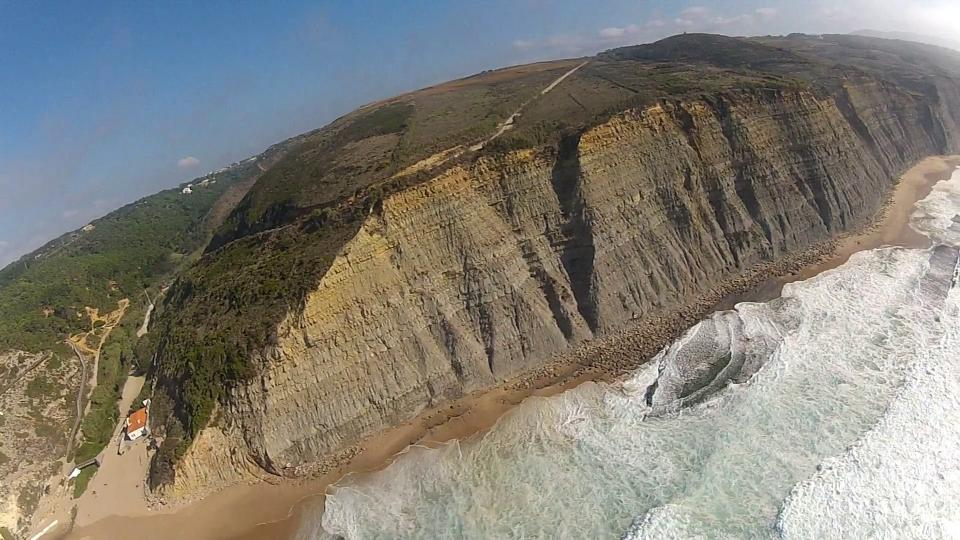
\includegraphics[width=0.8\linewidth]{FIGS/GoProVideo/Im1Ok.jpg}
\caption{First image of video  {\tt LM.mp4}}
\label{fig:GoProIm1}
\end{figure}


The issue we have to deal with are the following :

\begin{itemize}
   \item MicMac can process still images and not video;
   \item If we extract all the images, we will have too much redundant data, as can be seen
         on figure~\ref{fig:GoProCloseWave} with two consecutive images in superposition;
   \item The waves generate a lot of tie points (see figure~\ref{fig:GoProSIFT}) , which will be 
         a problem for photogrammetry as  they are 
         obviously not motionless relatively to the cliff;
          
   \item Currently with video, a lot of image are blurred (although it's not so much the case here ...);
   \item  There is no meta data embedded with video (at least, they disappear with the tool used to extract
          still images);
   \item  With this camera, there is a rolling shutter, so potentially each images has its own deformation;
\end{itemize}


\begin{figure}
\centering
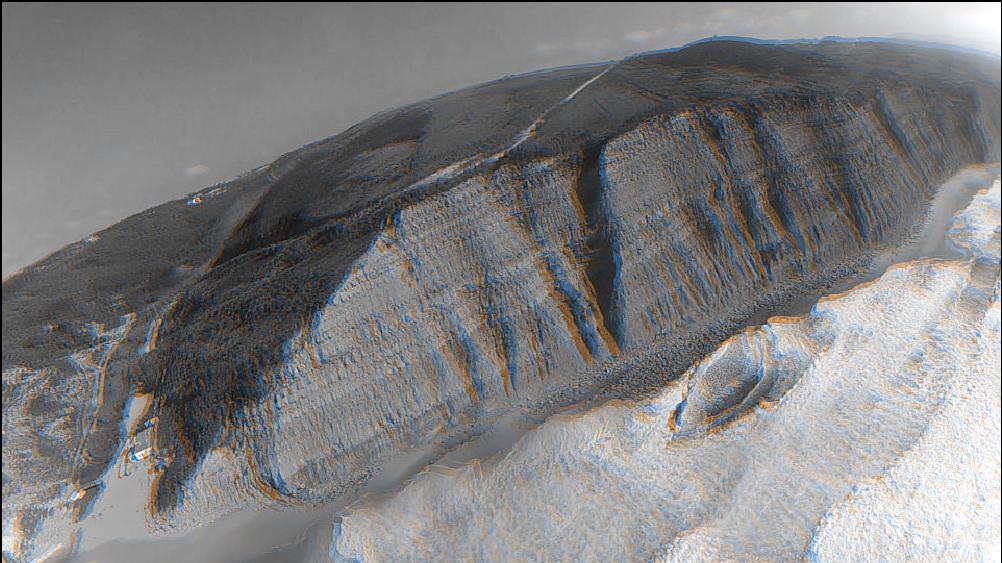
\includegraphics[width=0.80\linewidth]{FIGS/GoProVideo/Proches.jpg}
\caption{Two consecutive images of the video in superposition}
\label{fig:GoProCloseWave}
\end{figure}


\begin{figure}
\centering
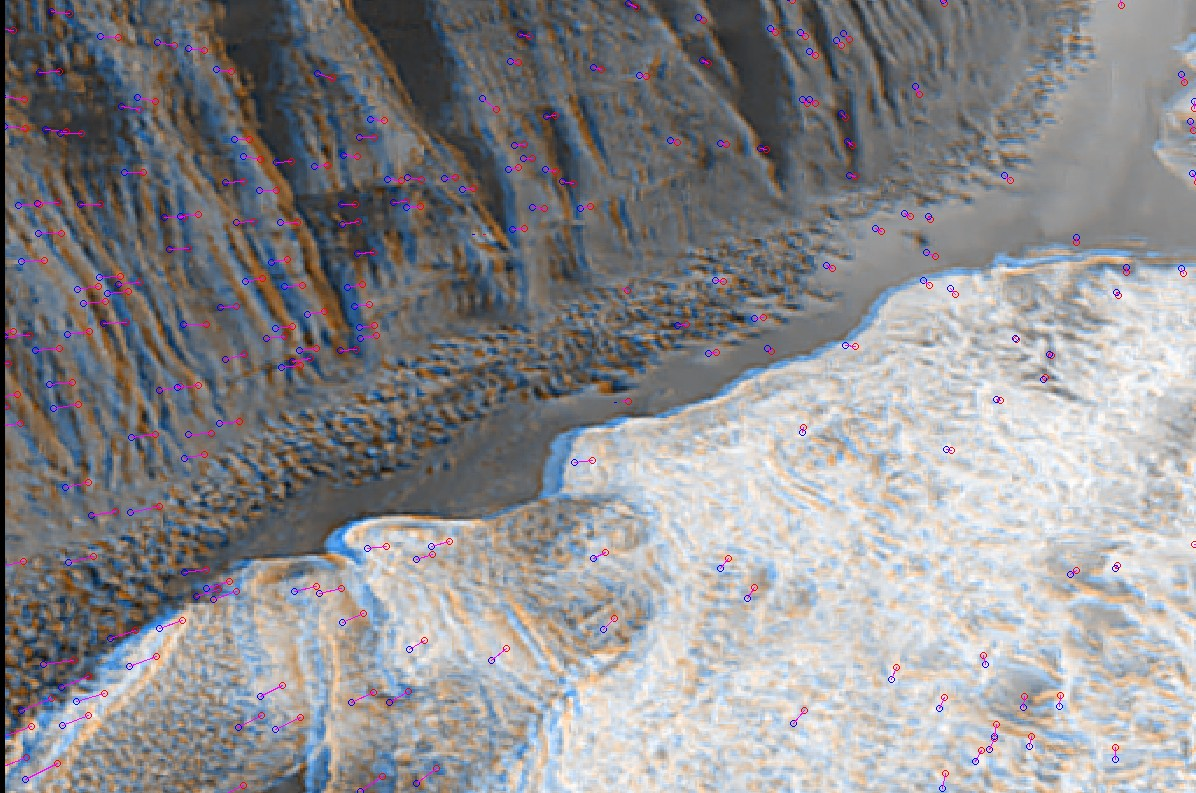
\includegraphics[width=0.90\linewidth]{FIGS/GoProVideo/SIFT.jpg}
\caption{Tie points from two extracted images}
\label{fig:GoProSIFT}
\end{figure}


\subsection{The commands}\label{GoProVideo:Commands}

The file {\tt Cmd.txt} in {\tt Documentation/FIGS/GoProVideo} contains the commands that have been used. They are :

\begin{verbatim}
# Develop all  images
ffmpeg -i LM.mp4  Im_0000_%5d_Ok.png

# Add missing xif
mm3d SetExif .*png F35=20 F=4.52 Cam=GoProVideoLM

# Select  approximatively 3 image / sec , preferring the sharpest one
mm3d DIV Im_0000_.*png Rate=3

#  Put the unselected images in basket
mkdir POUB
mv *Nl.png POUB/

#  Tie points adapted to  linear acquisition
Tapioca Line .*png 1000 10

# Compute a initial calibration; would not be necessary if we had already used this camera
mm3d Tapas  FishEyeBasic Im_0000_000.*png Out=Calib

#  Orient all the images
mm3d Tapas  FishEyeBasic Im_0000_.*png InCal=Calib Out=All0

# Generate a ply to visualize the scene
AperiCloud  .*png Ori-All0/

# Input a 2D mask that removes the sea
mm3d SaisieMasqQT  AperiCloud_All0.ply

#Filter the homologous point
mm3d HomolFilterMasq .*png OriMasq3D=Ori-All0/

# rename homologous points, the filtered one will be seen as the default
mv Homol HomolInit
mv HomolMasqFiltered/ Homol


# Compute orientation without the sea
Tapas   FishEyeBasic .*png InOri=Ori-All0/ Out=All1

# Free parameters
Campari  .*png  All1 All2 CPI1=1 FocFree=1 PPFree=1 AffineFree=1

# Generate the point cloud

mm3d C3DC BigMac .*png Ori-All2/ Tuning=0 Masq3D=AperiCloud_All2.ply ZoomF=1

\end{verbatim}



\subsection{Some comments}\label{GoProVideo:Comments}


\subsubsection{Developing still images with  {\tt ffmpeg}}

The software  {\tt ffmpeg} is a free open source package, we use it to extract the still images from video. Note :

\begin{itemize}
   \item We ask to extract \emph{all} the images, because we want to do  \emph{a posteriori} our own selection 
         of non-blurry images;
   \item To do this selection it is a requirement that the images use {\tt ffmpeg}  with the naming
          {\tt Im\_0000\_\%5d\_Ok.png}  (well the tool is still in very prototype state);

\end{itemize}


\subsubsection{Adding missing xif with {\tt SetExif}}

As there is no {\tt exif} information in the data set, we  add it to avoid the use of {\tt MicMac-LocalChantierDescripteur.xml}.
Note that is important to do it at the very beginning of the process, before using any other {\tt MicMac} tool, because after the xif 
will memorized in the {\tt Tmp-MM-Dir/.*xml} files


\subsubsection{Selecting sharpest images with  {\tt DIV}}

The {\tt DIV} command, makes selection of video images.
{\tt mm3d DIV Im\_0000\_.*png Rate=3} means : select approximately $3$ images per second 
(in fact one image out of $8$, assuming an initial rate $24$ images per second).  As some image have to be deleted,
this rate is only an approximation.

It the image is selected, its name is unchanged, while "deleted" images are renamed by replacing {\tt Ok} by {\tt Nl}.
As we don't want to use the deleted images, we put them in a "trash can" with the two lines 
{\tt mkdir POUB} and {\tt mv *Nl.png POUB/}.


\subsubsection{Standard orientation}

The three next line are quite standard MicMac processing :

\begin{itemize}
    \item {\tt  Tapioca Line .*png 1000 10} , compute tie point with command adapted to a linear acquisition;
    \item {\tt  mm3d Tapas  FishEyeBasic Im\_0000\_000.*png Out=Calib}, compute a first value of calibration , we
         use a fish-eye model adapted to this GoPro camera;
    \item {\tt  mm3d Tapas  FishEyeBasic Im\_0000\_.*png InCal=Calib Out=All0}, orient all the images, starting from
         the calibration
    \item {\tt  AperiCloud  .*png Ori-All0/} generate a ply file to visualize the scene and position of camera (see~\ref{fig:GoProOri0});

\end{itemize}

\begin{figure}
\centering
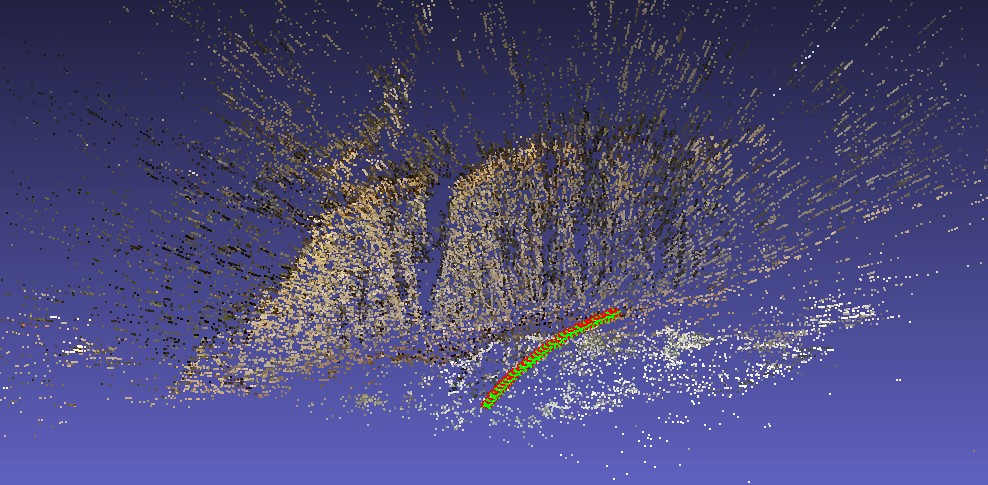
\includegraphics[width=0.80\linewidth]{FIGS/GoProVideo/Aperi000.jpg}
\caption{Orientation of images}
\label{fig:GoProOri0}
\end{figure}


\subsubsection{Seizing the waves}

With such acquisition, the best option to seize the location of the wave, is to seize in 3D. The other alternative, 
seize them in each images, would be much more time consuming. For this we can use the {\tt SaisieMasqQT} command,
see~\ref{Doc:SaisieMasqQT}.


\begin{figure}
\centering
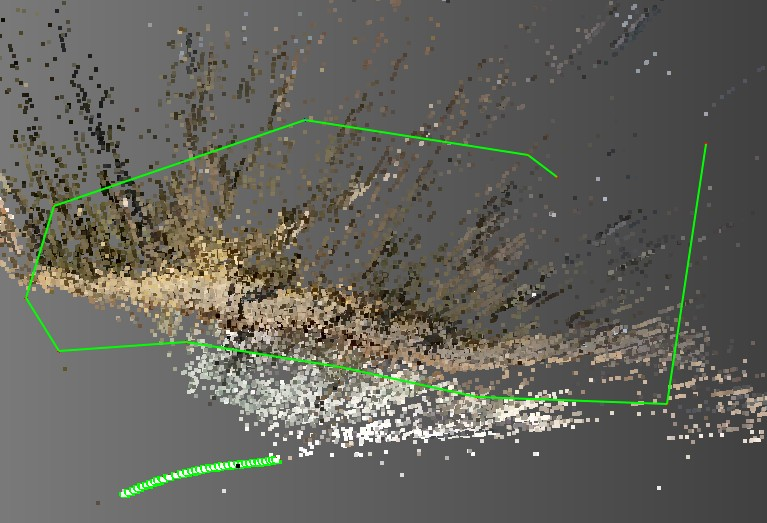
\includegraphics[width=0.80\linewidth]{FIGS/GoProVideo/Masq3D.jpg}
\caption{Seizing 3D masq  of the cliff}
\label{fig:GoProOri0}
\end{figure}

\subsubsection{Filtering homologous points}

We can now use the  {\tt HomolFilterMasq} command to select the tie points that are inside the $3$d masq.
We use the {\tt OriMasq3D} option to indicate the orientation (necessary to compute by ray intersection the $3$d point
associated to each tie point). By default, it assume that the mask has been seized on a {\tt AperiCloud} result, and
the default name of the $3$d mask is  here {\tt AperiCloud\_All2\_polyg3d.xml} .


\begin{figure}
\centering
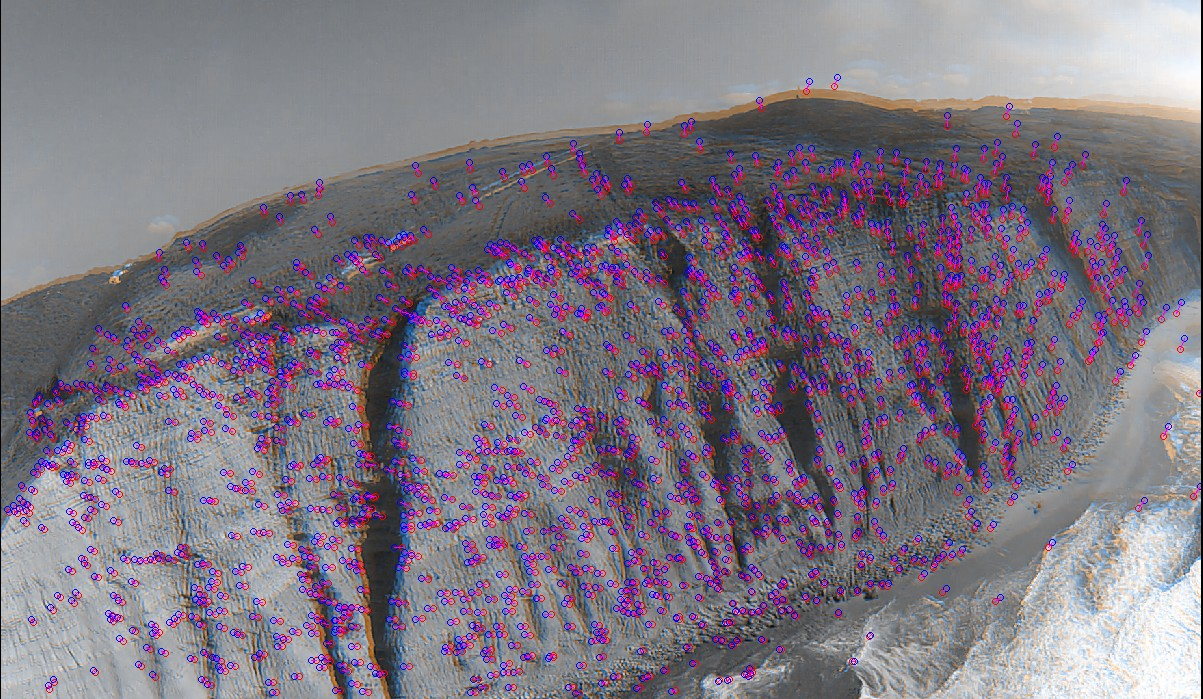
\includegraphics[width=0.90\linewidth]{FIGS/GoProVideo/SIFT2.jpg}
\caption{Tie points from  two extracted images after selection by $3$d masq}
\label{fig:GoProSIFT2}
\end{figure}

We have the to rename the homologous folder because by default all the MicMac command search the tie points 
in the folder {\tt Homol} :

\begin{verbatim}
mv Homol HomolInit
mv HomolMasqFiltered/ Homol
\end{verbatim}

\subsubsection{Final orientation}

Then we have two command to run to have the final orientation :


\begin{itemize}
   \item {\tt Tapas   FishEyeBasic .*png InOri=Ori-All0/ Out=All1} , here we run {\tt Tapas} taking into account
         the set of tie points without the sea;

   \item {\tt Campari  .*png  All1 All2 CPI1=1 FocFree=1 PPFree=1 AffineFree=1} , here we run {\tt Campari} with the option
         that select one internal calibration by images, we free the $0$ and $1$ degree parameter to take into account the
          rolling shutter (is it sufficient ? This is another story \dots).
\end{itemize}

And finally we can use the {\tt C3DC} command to generate a point cloud, a snapshot is presented on figure {\tt fig:GoProPlyFin}.

\begin{verbatim}
mm3d C3DC BigMac .*png Ori-All2/ Tuning=0 Masq3D=AperiCloud_All2.ply ZoomF=1
\end{verbatim}

\begin{figure}
\centering
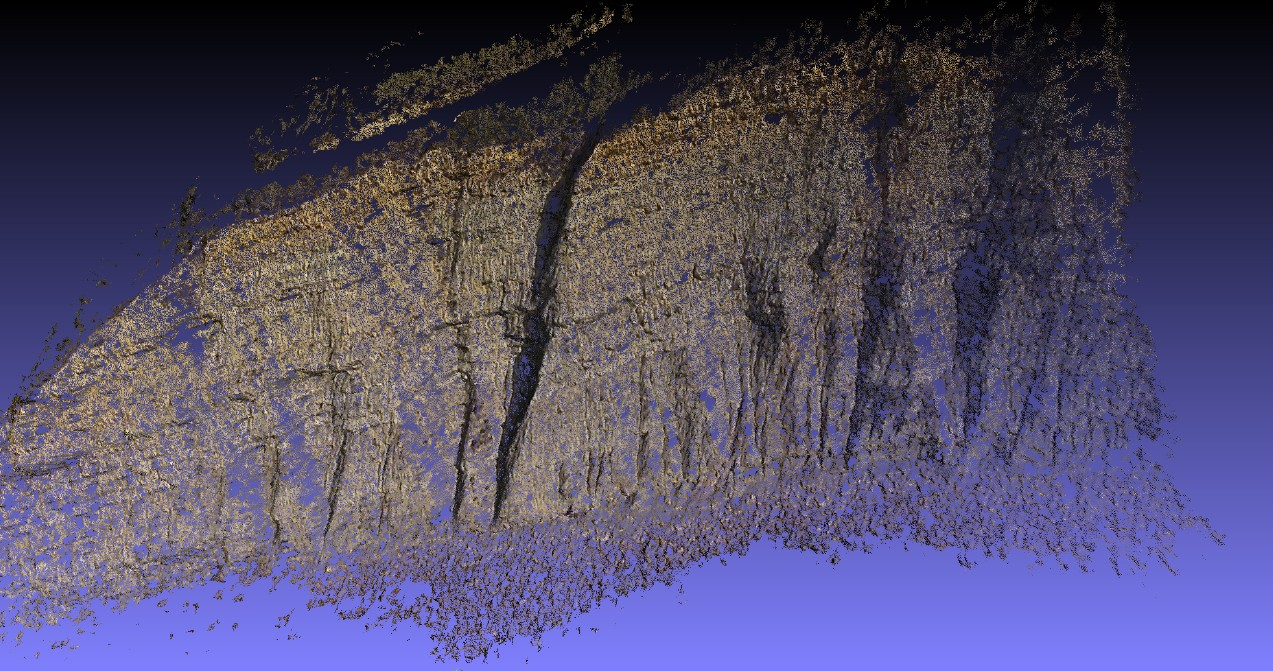
\includegraphics[width=0.90\linewidth]{FIGS/GoProVideo/PLY-Climb00.jpg}
\caption{Tie points from  two extracted images after selection by $3$d masq}
\label{fig:GoProPlyFin}
\end{figure}
%%%%%%%%%%%%%%%%%%%%%%%%%%%%%%%%%%%%%%%%%%%%%%%%%%%%%%%%%%%%%%%%%%%%%%%%%%%%%%%%%%%%%%%%%%%%%%%%%%%%%%%%%%
\section{The satellite data set}\label{sec:usecase:satel}
%
\subsection{Description of the data}
%
A Pleiades tristereo is processed in the following. The images are part of a sample dataset disseminated by the Airbus Defence and Space and can be downloaded from http://www.geo-airbusds.com/en/23-sample-imagery 
\subsection{From 2D images to 3D objects -- the processing commands}
%
Unless you work with MicMac and the Kakadu license, the orignal JPEG2000 images must be  converted to tiff. The otb library\footnote{https://www.orfeo-toolbox.org/} allows for the conversion using the command below: 
\begin{verbatim}
otbcli_Convert -in image.jp2 -out image.tif uint16
\end{verbatim}
%
The tie points can now be extracted from the images:
\begin{verbatim}
mm3d Tapioca All .*.tif 10000  
\end{verbatim}
%
Next, as mentioned in Section~\ref{sec:rpcBundle}, the input files with rational polynomial coefficients ought to be converted to a MicMac readable format, and the processing coordinate system defined:
\begin{verbatim}
mm3d Convert2GenBundle "IMG_PHR1A_P_20120225002(.*)_SEN_PRG_FC_51(.*)-001_R1C1.tif"
"RPC_PHR1A_P_20120225002\$1_SEN_PRG_FC_51\$2-001.XML" RPC-deg1 ChSys=WGS84toUTM.xml Degre=1
\end{verbatim}
%
which is equivalent of independently running the same command for three images:
%
\begin{verbatim} 
mm3d Convert2GenBundle IMG_PHR1A_P_201202250025329_SEN_PRG_FC_5110-001_R1C1.tif
RPC_PHR1A_P_201202250025329_SEN_PRG_FC_5110-001.XML RPC-deg1 ChSys=WGS84toUTM.xml Degre=1
mm3d Convert2GenBundle IMG_PHR1A_P_201202250025599_SEN_PRG_FC_5108-001_R1C1.tif
RPC_PHR1A_P_201202250025599_SEN_PRG_FC_5108-001.XML RPC-deg1 ChSys=WGS84toUTM.xml Degre=1
mm3d Convert2GenBundle IMG_PHR1A_P_201202250026276_SEN_PRG_FC_5109-001_R1C1.tif
RPC_PHR1A_P_201202250026276_SEN_PRG_FC_5109-001.XML RPC-deg1 ChSys=WGS84toUTM.xml Degre=1
\end{verbatim}
%
Generally you one would prefer to use the regular expression rather than run repeateadly the same command for each image as the latter is very error-prone. The content of the coordinate system file renders:
\begin{verbatim}
<SystemeCoord>
  <BSC>
     <TypeCoord>eTC_Proj4</TypeCoord>
     <AuxStr>+proj=utm +zone=55 +south +ellps=WGS84 +datum=WGS84 +units=m +no_defs</AuxStr>
  </BSC>
</SystemeCoord> 
\end{verbatim}
%
Given the extracted tie points, the RPC bundle adjustment can proceed with the simplified tool {\tt Campari} (see Subsection~\ref{CAMPARI}):
\begin{verbatim}
mm3d Campari .*.tif RPC-deg1 RPC-deg1_adj
\end{verbatim}
%   
Refer to section~\ref{subsub:rpcCampari} for a more detailed description of the adjustment algorithm. Provided the results deliver satisfying residuals (in the presented case reflecting only the reprojection errors of the tie points, but more generally also determining the adherence of the data to some control information), the dense matching can be carried out. Nevertheless, it is worthwhile to verify the refined orientation between pairs of images using the {\tt mm3d MMTestOrient} (see Subsection~\ref{CheckOri}):
\begin{verbatim}
mm3d MMTestOrient IMG_PHR1A_P_201202250025329_SEN_PRG_FC_5110-001_R1C1.tif 
IMG_PHR1A_P_201202250025599_SEN_PRG_FC_5108-001_R1C1.tif Ori-RPC-deg1_adj GB=1 ZMoy=0 ZInc=500
\end{verbatim}
%
In case one would want to use the adjusted orientation in some external software, it is possible to recompute the RPCs with the command:
\begin{verbatim}
mm3d SateLib RecalRPC Ori-RPC-deg1_adj/
GB-Orientation-IMG_PHR1A_P_201202250025329_SEN_PRG_FC_5110-001_R1C1.tif.xml
\end{verbatim}
The DSM generation is handled, again, by the simplified tool {\tt Malt} (see Subsection~\ref{subsec:Malt}): 
\begin{verbatim}
mm3d Malt UrbanMNE .*.tif Ori-RPC-deg1_adj ZMoy=0 ZInc=500
\end{verbatim}
%

\subsection{Understanding the bundle adjustment output ({\tt Campari})} 
%
The adjustment result is stored inside the {\texttt{Ori-RPC-deg1\_adj}} directory. Understanding the bundle adjustment message printed to the screen (and additionally stored inside a {\tt Residus.xml} file) is already explained in subsection~\ref{subsec:Apero:msg}. The output directory contains files with the original RPCs (all files with the prefix {\tt UnCorExtern-}), and the corresponding files with adjusted orientation parameters (all files with the prefix {\tt GB-}). The {\tt GB-} files contain:
\begin{itemize}
\item {\tt NameCamSsCor}, the filepath to the original RPCs;
\item {\tt NameIma}, the name of the image that the file corresponds to;
\item {\tt SysCible}, the definition of the coordinate system used in the processing (proj4 format);
\item {\tt DegreTot}, the degree of the adjustable 2D polynomial correction function;
\item {\tt Center}, the polynomial's normalizing shift (in pixels);
\item {\tt Ampl}, the polynomial's normalizing amplitude;
\item {\tt CorX}, the polynomial's normalized x-coefficients;
\item {\tt CorY}, the polynomial's normalized y-coefficients;
\item {\tt Monomes}, three values corresponding to respective polynomial terms (e.g. \texttt{<Monomes>-0.94 0 1</Monomes>} interprets as $-0.94 \cdot x^0 \cdot y^1 $). 
\end{itemize}
The avoid numerical instabilities of the polynomial functions, the {\tt Center} and {\tt Ampl} parameters normalize the image space such that all observations are contained within the range $<-1,1>$. The user can visualize the correction polynomial functions with 
\begin{verbatim}
mm3d SateLib SATD2D Ori-RPC-deg1_adj/GB-Orientation-
                    IMG_PHR1A_P_201202250025329_SEN_PRG_FC_5110-001_R1C1.tif.xml
\end{verbatim}
%
The tool produces images of displacements separately in x, y and combined xy directions (see Fig.~\ref{fig:satPoly2d}), and prints to the screen the minimum/maximum values in pixels:
\begin{verbatim}
displacement in x:  GMin,Gax -0.96187676315564 -0.919344454426481
displacement in y:  GMin,Gax -0.542404322159884 0.234261700467604
displacement in xy:  GMin,Gax 0.919404732429707 1.06767206091774
\end{verbatim}
%   
\begin{figure}[h!]
\centering

\includegraphics[width=0.95\linewidth]{FIGS/Satellites/SATD2D.png}
\caption{Displacements in image space caused by the correcting polynomial functions in image \texttt{IMG\_PHR1A\_P\_201202250025329\_SEN\_PRG\_FC\_5110-001\_R1C1.tif}. Displacement magnitude (a) along the x-coordinate, (b) along the y-coordinate, (c) combined along both coordinate directions.}
\label{fig:satPoly2d}
\end{figure}
%
\subsection{Understanding the bundle adjustment validation output ({\tt MMTestOrient})}
% 
The output of the {\tt MMTestOrient} tool described in Section~\ref{sec:MMTestOri} is shown in Fig.~\ref{fig:satMMTestOri}. Using the tool {\tt mm3d StatIm}, some basic image statistics can be obtained allowing the interpretation of the outcome:
\begin{verbatim}
mm3d StatIm GeoI-Px/Px2_Num16_DeZoom2_Geom-Im.tif [1000,1000] Sz=[8000,4000]
\end{verbatim}
%
The command above calculates the mean, the standard deviation, as well as min/max parallax values over the bounding box anchored at [1000,1000], of size [8000,4000]. Because the input parallax image is at the \texttt{DeZoom=2}, rather than the full resolution, all values must be multiplied by two. The image statistics over the selected bounding box in pixels are then:
\begin{verbatim}
ZMoy=0.064 ; Sigma=0.122
ZMinMax=[-2.70 , 2.03]
\end{verbatim}
%   
The two most relevant statistics are: the mean transverse parallax which is very close to zero, and the sigma equal to $\approx 0.1$ pixel. The min/max values are relief-related and occur in places of low correlation, e.g. on vegetation, water surfaces, or in places of shadows and occlusions. The magnitude of systematic pattern visible in Fig.~\ref{fig:satMMTestOri} remains at the level of the sigma value, hence well below the adjustment precision ($~0.6$ pixel). The user is encouraged to use \texttt{mm3d Vino} tool to display very big image files.
%
\begin{figure}[h!]
\centering
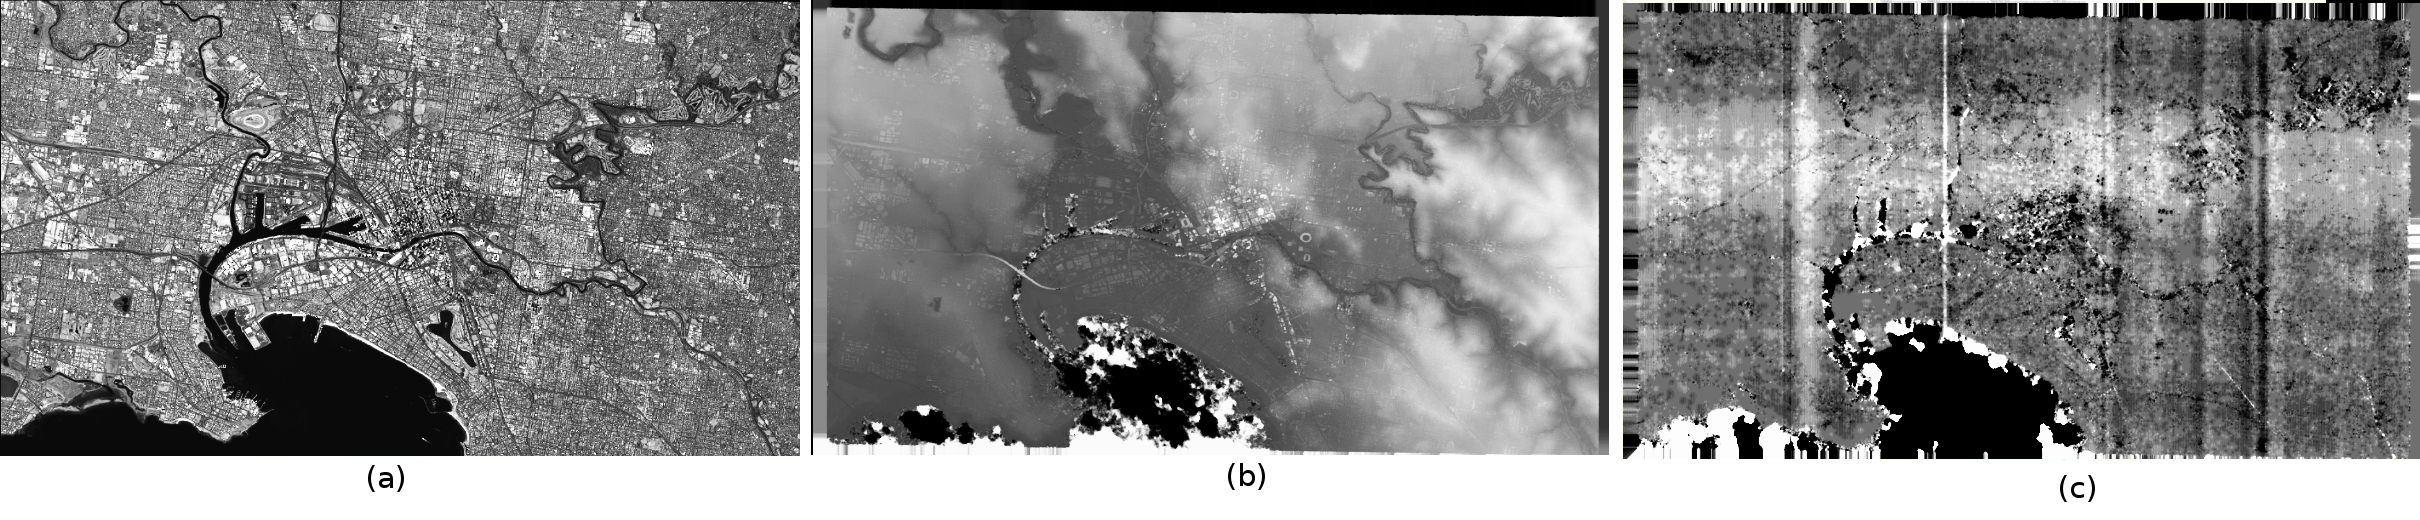
\includegraphics[width=0.95\linewidth]{FIGS/Satellites/IMG_Px1_Px2_Num16.png}
\caption{(a) A satellite image, (b) the epipolar parallax (\texttt{Px1\_Num16\_DeZoom2\_Geom-Im.tif}), (c) the transverse parallax (\texttt{Px2\_Num16\_DeZoom2\_Geom-Im.tif}).}
\label{fig:satMMTestOri}
\end{figure}

%%%%%%%%%%%%%%%%%%%%%%%%%%%%%%%%%%%%%%%%%%%%%%%%%%%%%%%%%%%%%%%%%%%%%%%%%%%%%%%%%%%%%%%%%%%%%%%%%%%%%%%%%%

\section{The Viabon dataset}
The directory {\tt Viabon/} in {\tt /micmac\_data/ExempleDoc/} contains a set of data which will allow us to perform a direct-georeferencing of images based on embedded GPS data. Below we will detail all the necessary steps to achieve maximum ground accuracy, here, in the range of {\tt 1-2 cm}. First, we will compute different GPS trajectories in order to make comparisons and in a second time we will be interested in the fusion of these results with the photogrammetric processing part.\newline

This UAS acquisition has been performed by the surveying service of {\tt Vinci-Construction-Terrassement}\footnote{\url{http://www.vinci-construction-terrassement.com/}}. A {\tt DJI-F550}\footnote{\url{http://dl.djicdn.com/downloads/flamewheel/en/F550_User_Manual_v2.0_en.pdf}} hexa-copter has been used to achieve the flight. The images were acquired by the {\tt IGN} panchromatic light camera developed at the {\tt LOEMI}\footnote{Opto-Electronics, Instrumentation and Metrology Laboratory} laboratory. The GPS on-board raw measurements were acquired by the {\tt GeoCube}, a multi-sensor geo-monitoring system developed at the same laboratory.\newline

The file {\tt Viabon/Pipeline-Viabon.txt} contains all command lines related to this work-flow. The data in {\tt Viabon/} directory consist of:
\newline
\begin{itemize}
\item 73 nadir images in {\tt .tif} raw format
\item {\tt 15073106.obs} rinex file of rover receiver
\item {\tt 00012120.15O} rinex file of pivot/base station
\item {\tt ct19212z.15o} rinex file of closest {\tt RGP}\footnote{GNSS Permanent Network: \url{http://rgp.ign.fr/}} network station
\item {\tt ct19212z.15n} GPS satellites navigation file
\item {\tt ct19212z.15g} Glonass satellites navigation file
\item {\tt igs08.atx} satellites and receiver antennas calibration values
\item {\tt CpleImgs.xml} images couples for tie points computation
\item {\tt Pts\_GeoC.txt} ground points coordinates
\item {\tt MesImages.xml} image measurements of ground points
\item {\tt GCP\_LA\_Calib-RTL.xml} 1 ground control point for lever-arm calibration 
\item {\tt CPs\_LA\_Calib-RTL.xml} check points to estimate lever-arm calibration accuracy
\item {\tt Reduced\_GCPs-RTL.xml} reduced number of ground control points for classical georeferencing
\item {\tt Reduced\_CPs-RTL.xml} reduced check points to estimate GCPs based georeferencing accuracy
\item {\tt SysCoRTL.xml} file for system coordinates transformation 
\end{itemize}

\begin{figure}[H]
    \begin{center}
    \setlength{\unitlength}{0.5cm}
    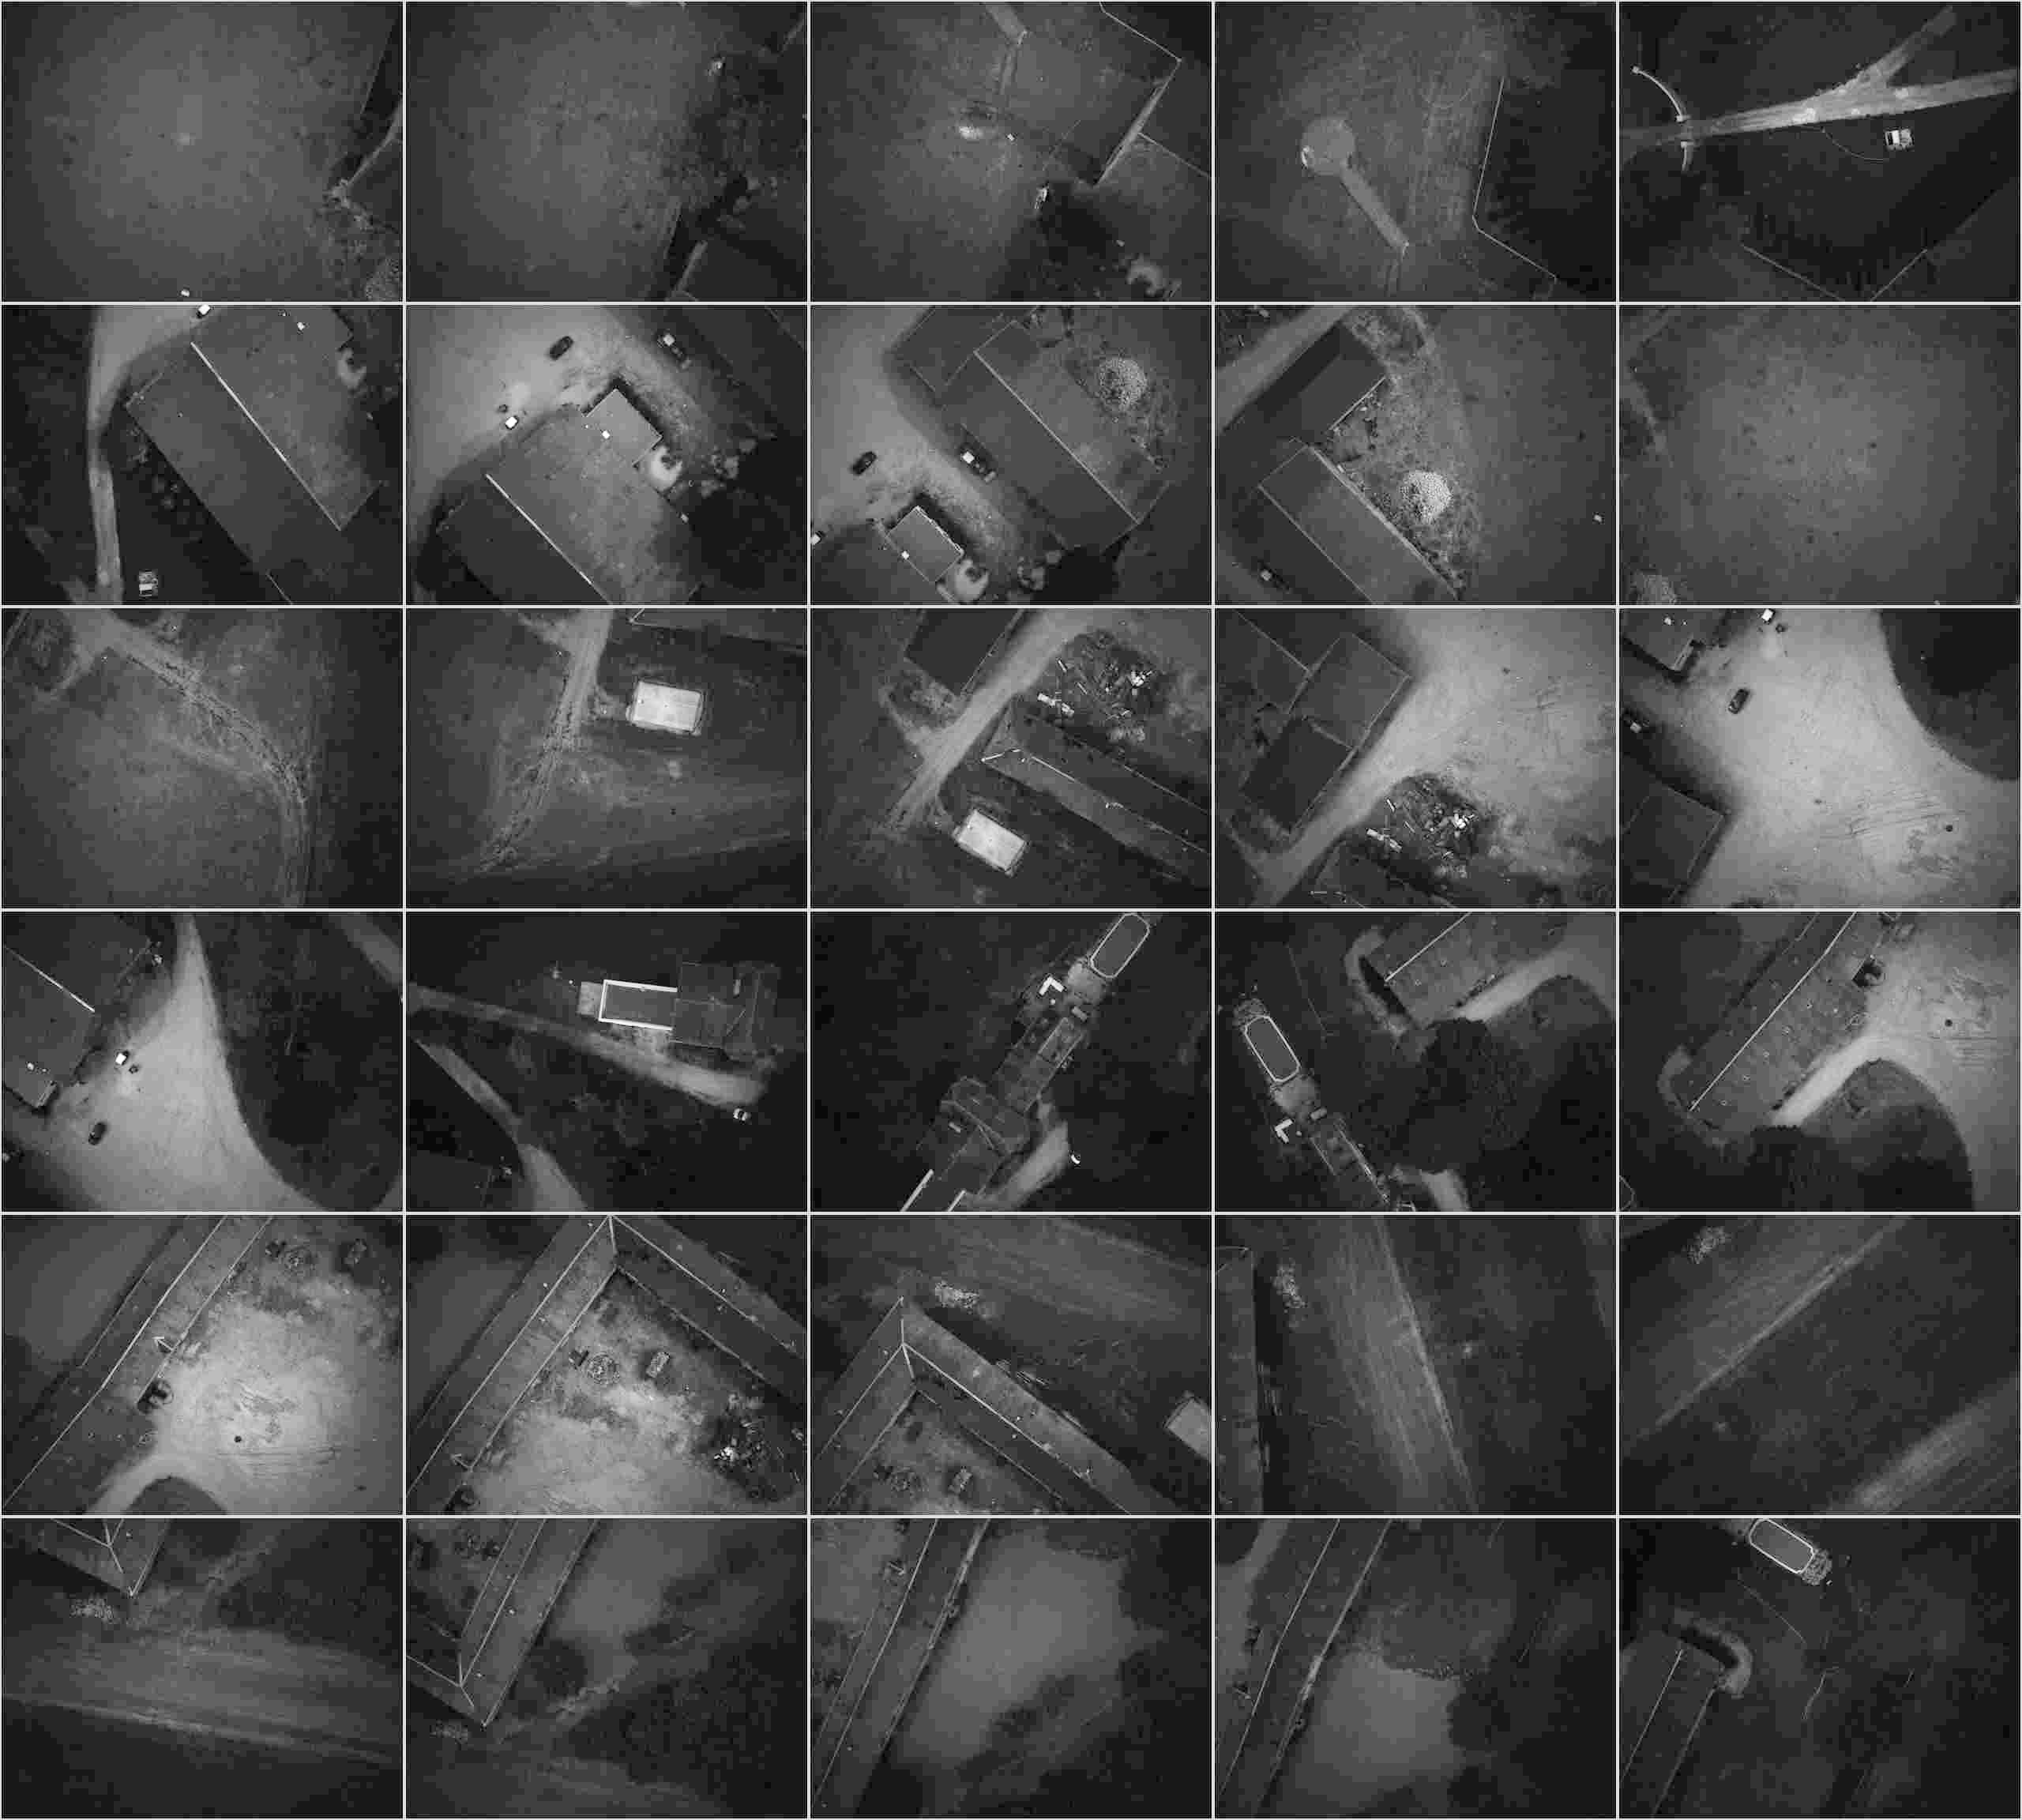
\includegraphics[width=0.5\linewidth]{FIGS/Viabon/panel.jpg}
    \end{center}
    \caption{The Viabon dataset}
    \label{fig:iris}
\end{figure}

\subsection{Processing GPS data}
For GPS data processing we will use {\tt RTKLIB}\footnote{\url{http://www.rtklib.com/}} an open-source software. {\tt RTKLIB} consists of several modules ({\tt convbin}, {\tt rnx2rtkp}, {\tt rtkrcv}, ...etc). We will only use {\tt rnx2rtkp} which will allow us to do post-processing of our data based on different positioning modes.

\subsubsection{Compile {\tt MicMac} with {\tt RTKlib}}
To use {\tt rnx2rtkp}, if compiling {\tt MicMac} from sources, run {\tt cmake} with {\tt -DBUILD\_RNX2RTKP} option activated as follows:

\begin{verbatim}
cmake ../ -DBUILD_RNX2RTKP=ON
\end{verbatim}

\subsubsection{Base station processing}\label{proc_pivot}
First we use {\tt GpsProc} command to compute the position of the base station which will be used to process the UAV trajectory. The data recorded by the on-board GPS receiver are single-frequency data. This implies, for optimal accuracy, having a base station within a radius of $\sim$ 10 km. A pivot station has been installed near the acquisition area (file {\tt 00012120.15O}) . This station is a multi-constellation dual-frequency {\tt Novatel GNSS} receiver. The position of this pivot station is estimated relatively to a reference station of the French permanent {\tt GNSS} network (file {\tt ct19212z.15o}).\newline

First we estimate the position of the pivot station:

\begin{verbatim}
mm3d TestLib GpsProc './' static 00012120.15O ct19212z.15o ct19212z.15n NavSys=5 
     GloNavFile=ct19212z.15g Freq=l1_l2 AntFileRCV=igs08.atx AntFileSATs=igs08.atx 
     AntBType=TRM55971.00
\end{verbatim}

First mandatory argument is the current directory. Second mandatory argument is the processing mode. Here we tell the software that we want to estimate a position of {\tt static} measurements. Third mandatory argument is rinex file of known station, here {\tt CT19}\footnote{\url{http://rgp.ign.fr/STATIONS/\#CT19}} of French Permanent GNSS Network. Last mandatory argument contains GPS constellation satellites navigation parameters. For optional arguments, {\tt NavSys=5} means that we use both constellations {\tt GPS} and {\tt Glonass} with respect to {\tt RTKlib} conventions\footnote{\url{http://www.rtklib.com/rtklib_document.htm}}. In this case, we need then to give the navigation file for Glonass constellation too using the optional argument {\tt GloNavFile=ct19212z.15g}. Once both receivers are dual-frequency receivers, we perform the processing in both frequencies, this is specified with the optional argument {\tt Freq=l1\_l2}. Finally, we use optional arguments to perform antennas corrections, and we specify the antenna model for {\tt CT19} as the antenna is listed in {\tt igs08.atx} file. Here, 3 files are created:\newline
\begin{itemize}
\item {\tt ./rtkParamsConfigs.txt} a summary of the options used by {\tt rnx2rtkp}
\item {\tt ./Output\_static.txt} the result in {\tt RTKLIB} format
\item {\tt ./Output\_static.xml} the result in an XML format for {\tt MicMac} internal using
\end{itemize}

\subsubsection{UAV trajectories processing}
All UAVs board at least a single-frequency GPS chip\footnote{For example u-blox NEO-7N} that receives the L1\footnote{1575.42 MHz} C/A\footnote{Coarse/Acquisition} code signal. First, we process a trajectory based solely on this data in order to evaluate its accuracy in the case our system delivers only available code positions:

\begin{verbatim}
mm3d TestLib GpsProc './' single 15073106.obs NONE ct19212z.15n
\end{verbatim}

Here the second mandatory argument, corresponding to positioning mode, value is {\tt single}. This means that we process only rover code measurements. Next mandatory argument is the rinex file of raw measurements of rover receiver ({\tt 15073106.obs}). Any differential processing is done here, we give the value {\tt NONE}. Last mandatory argument correspond to GPS constellation satellites navigations parameters. The trajectory is saved in {\tt RTKlib} and {\tt MicMac} respectively in file {\tt Output\_single.txt} and {\tt Output\_single.xml}.\newline

Assume that the GPS module of the UAV autopilot allow us to record L1 C/A code raw data. Then, it is possible to process a trajectory in differential mode based on code data (the same data used for navigation of the UAV) to improve the accuracy of the estimated trajectory:

\begin{verbatim}
mm3d TestLib GpsProc './' dgps 15073106.obs 00012120.15O ct19212z.15n 
     AntBPosType=XYZ StaPosFile=Output_static.xml
\end{verbatim}

The positioning mode is {\tt dgps}. Here we give as input file rinex raw measurements of pivot station ({\tt 00012120.15O}). As the position has been estimated in \ref{proc_pivot}, optional arguments {\tt StaPosFile=Output\_static.xml} is used to give reference position of the pivot and {\tt  AntBPosType=XYZ} specifies the format of the given position.\newline

The GPS chip embedded in the {\tt GeoCube} is a {\tt u-blox LEA-6T-0-001}\footnote{\url{https://www.u-blox.com/en/product/neolea-6t}} model. This GPS module allows recording carrier-phase raw data. As noise measurement on carrier-phase is much less important than on code measurements, we perform a differential processing based on raw phase data:

\begin{verbatim}
mm3d TestLib GpsProc './' kinematic 15073106.obs 00012120.15O ct19212z.15n 
     AntBPosType=XYZ StaPosFile=Output_static.xml
\end{verbatim}

The positioning mode value is {\tt kinematic}. As for previous command, we give reference position of pivot station using optional arguments. Carrier-phase trajectory is stored in the files {\tt Output\_kinematic.xml} and {\tt Output\_kinematic.txt}.


\subsection{Computing tie points}
{\tt CpleImgs.xml} file is used with the {\tt mm3d Tapioca} command to accelerate tie points extraction. This file contains all pairs of overlapping images. We perform tie points extraction based on images sub-sampled by a factor of 3:

\begin{verbatim}
mm3d Tapioca File CpleImgs.xml 1300
\end{verbatim}

Visualize tie points between 2 images using {\tt mm3d SEL} command:

\begin{verbatim}
mm3d SEL './' image_002_00069.tif image_002_00070.tif KH=NB
\end{verbatim}

\begin{figure}[H]
    \begin{center}
    \setlength{\unitlength}{0.5cm}
    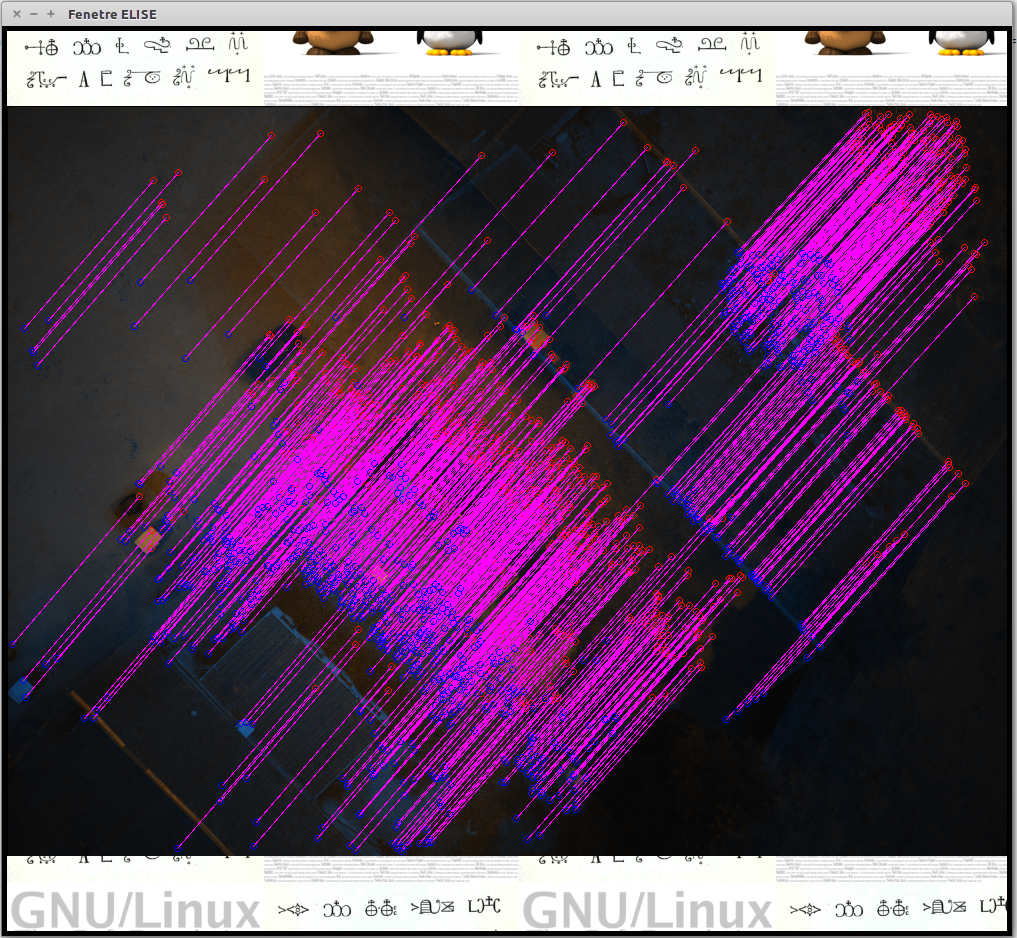
\includegraphics[width=0.5\linewidth]{FIGS/Viabon/sel.png}
    \end{center}
    \caption{Tie points visualization}
    \label{fig:sel}
\end{figure}

\subsubsection{Computing exterior orientation}

To speed up the relative orientation computation, the images bloc is initialized using {\tt mm3d Martini} command used for large bloc. {\tt mm3d AperiCloud} command is used to export images estimated exterior parameters in a {\tt .ply} file format and one can visualize it using the free and open-source software {\tt meshlab}:

\begin{verbatim}
mm3d Martini "image_002_00*.*tif"
mm3d AperiCloud "image_002_00*.*tif" Martini
meshlab AperiCloud_Martini.ply
\end{verbatim}

\begin{figure}[H]
    \begin{center}
    \setlength{\unitlength}{0.5cm}
    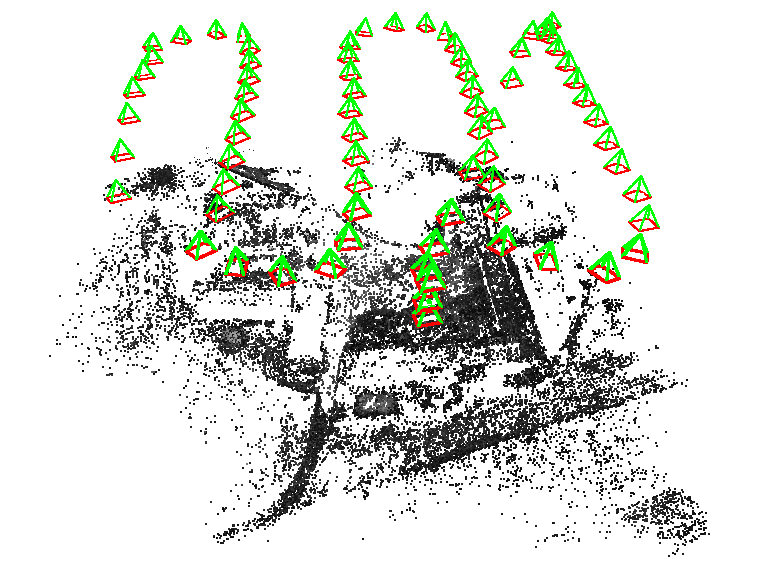
\includegraphics[width=0.5\linewidth]{FIGS/Viabon/apericloud.png}
    \end{center}
    \caption{Bloc visualization}
    \label{fig:sel}
\end{figure}


The command {\tt mm3d Tapas} is used to perform relative orientation based on the bloc initialization computed before and we use the {\tt RadialStd} camera model which has 8 degrees of freedom:

\begin{verbatim}
mm3d Tapas RadialStd "image_002_00*.*tif" InOri=Martini Out=All-RS
mm3d AperiCloud "image_002_00*.*tif" All-RS
meshlab AperiCloud_All-RS.ply
\end{verbatim}

\subsubsection{GPS positions \& Camera centers matching}
Time synchronization of sensors (camera \& GPS) was conducted in the laboratory. The electronic delay is negligible ($\sim$ 0.5 ms) and the GPS receiver is in charge of triggering the camera. This means that image centers are aligned with GPS positions. However, sampling of both trajectories is different, the camera does not have an internal clock (no time information in {\tt exif} meta-data) and camera triggering is not dated in the GPS time-scale. The identification of corresponding positions is done by computing the best correlation score of distances ratios curves and by testing all possible time shifts using {\tt mm3d TestLib MatchCenters}:

\begin{verbatim}
mm3d TestLib MatchCenters './' Ori-All-RS/ Output_single.xml "image_002_00*.*tif"
mm3d TestLib MatchCenters './' Ori-All-RS/ Output_dgps.xml "image_002_00*.*tif"
mm3d TestLib MatchCenters './' Ori-All-RS/ Output_kinematic.xml "image_002_00*.*tif"
\end{verbatim}

The output files ({\tt Ori-Output\_single.txt}, ...) gives for each image the corresponding GPS position. Then, the {\tt mm3d OriConvert} command is used to convert the resulting file into {\tt Ori-XXX/ .xml} format orientations folder and performing at the same time a coordinate system transformation using optional argument {\tt ChSys}:

\begin{verbatim}
mm3d OriConvert "#F=N_X_Y_Z" Ori-Output_single.txt Nav-Code ChSys=GeoC@SysCoRTL.xml
mm3d OriConvert "#F=N_X_Y_Z" Ori-Output_dgps.txt Nav-DCode ChSys=GeoC@SysCoRTL.xml
mm3d OriConvert "#F=N_X_Y_Z" Ori-Output_kinematic.txt Nav-DPhase ChSys=GeoC@SysCoRTL.xml
\end{verbatim}

At this step we performed different GPS trajectories calculations. We also have a set of images positions/orientations computed based on bundle block adjustment using only tie points. Also, we have for each GPS trajectory solution (absolute code, differential code and differential carrier-phase) correspondences between GPS positions and images centers that will allow us to convert the relative external orientation into absolute one.

\subsubsection{Images georeferencing}\label{sec_basc}
Let's first convert Ground Control Points file from {\tt .txt} to {\tt .xml MicMac} format using the {\tt mm3d GCPConvert} command and performing at the same time a coordinate system transformation using the optional argument {\tt ChSys}:

\begin{verbatim}
mm3d GCPConvert "#F=N_X_Y_Z_Ix_Iy_Iz" Pts_GeoC.txt Out=AllPts-RTL.xml 
     ChSys=GeoC@SysCoRTL.xml
\end{verbatim}

Here we start by comparing raw similarity transformations using different GPS processing results performed above. First for absolute navigation using code measurements. The command {\tt mm3d CenterBascule} is used to generate absolute orientations, here stored in the folder {\tt Ori-Bascule-RS-Code/}. Then the command {\tt mm3d GCPCtrl} is used to control accuracy on the ground by computing residuals on all available points here all considered as check points:

\begin{verbatim}
mm3d CenterBascule "image_002_00*.*tif" Ori-All-RS/ Ori-Nav-Code/ Bascule-RS-Code
mm3d GCPCtrl "image_002_00*.*tif" Ori-Bascule-RS-Code/ AllPts.xml MesImages.xml

============================= ERRROR MAX PTS FL ======================
   ||    Value=140.12 for Cam=image_002_00100.tif and Pt=7 ; MoyErr=130.967
======================================================================
=== GCP STAT ===  Dist,  Moy=1.52601 Max=1.65398
\end{verbatim}
% XYZ , MoyAbs=[0.902746,1.12483,0.466344] 
%       Max=[1.10388,1.42946,0.557705] 
%       Bias=[-0.902746,1.12483,0.466344]


Here for differential code trajectory processed:

\begin{verbatim}
mm3d CenterBascule "image_002_00*.*tif" Ori-All-RS/ Ori-Nav-DCode/ Bascule-RS-DCode
mm3d GCPCtrl "image_002_00*.*tif" Ori-Bascule-RS-DCode/ AllPts.xml MesImages.xml

============================= ERRROR MAX PTS FL ======================
   ||    Value=71.3855 for Cam=image_002_00058.tif and Pt=1 ; MoyErr=53.4976
======================================================================
=== GCP STAT ===  Dist,  Moy=0.640848 Max=0.844784
\end{verbatim}

% XYZ , MoyAbs=[0.144261,0.576277,0.1939] 
%       Max=[0.271985,0.819833,0.332405] 
%       Bias=[-0.0568969,-0.576277,0.1939]


Here for differential carrier-phase trajectory processed:

\begin{verbatim}
mm3d CenterBascule "image_002_00*.*tif" Ori-All-RS/ Ori-Nav-Dphase/ Bascule-RS-DPhase
mm3d GCPCtrl "image_002_00*.*tif" Ori-Bascule-RS-DPhase/ AllPts.xml MesImages.xml

============================= ERRROR MAX PTS FL ======================
   ||    Value=40.8538 for Cam=image_002_00076.tif and Pt=4 ; MoyErr=21.3675
======================================================================
=== GCP STAT ===  Dist,  Moy=0.32083 Max=0.470131
\end{verbatim}
% XYZ , MoyAbs=[0.107108,0.130186,0.244281] 
%       Max=[0.285027,0.371262,0.284798] 
%       Bias=[0.0423598,0.107904,0.244281]


We notice after the three georeferencing computations that the reprojection error is improved by a factor of $\sim$ $2.5$ (for this dataset) when code measurements are used in differential mode ({\tt dgps}. The best georeferencing results are obtained using the calculated trajectory based on differential carrier-phase measurements ({\tt MoyErr $\sim$ 21 px}).

%%%%%%%%%%%%%%%%%%%%%%%%%%%%%%%%%%%%%%%%%%%%%%%%%%%%%%%%%%%%%%%%%%%%%%%%%%%%%%%%%%%%%%%%%%%%%%%%%%%%%%%%%%%%%%%%%%%%
\subsubsection{Bundle Bloc Adjustment with GPS observations and lever-arm offset}
Here we perform, with the {\tt mm3d Campari} command, a heterogeneous compensation using tie points and GPS camera positions estimated using GPS observations. In addition, here we take into account the fact that camera optical center and GPS antenna phase center are separated by a vector called the lever-arm offset using the optional argument {\tt GpsLa}.\newline

For bundle block adjustment using C/A code positions, planimetric uncertainty is fixed to $3\ m$ and vertical component uncertainty is fixed to $5\ m$ in the optional argument {\tt EmGPS}:

\begin{verbatim}
mm3d Campari "image_002_00*.*tif" Ori-Bascule-RS-Code/ Compense-RS-Code-La
     EmGPS=[Ori-Nav-Code/,3,5] GpsLa=[0,0,0]
     
mm3d GCPCtrl "image_002_00*.*tif" Ori-Compense-RS-Code-La/ AllPts-RTL.xml MesImages.xml

LA: [0.263412,0.034836,-2.03753]

============================= ERRROR MAX PTS FL ======================
   ||    Value=212.782 for Cam=image_002_00110.tif and Pt=10 ; MoyErr=195.637
======================================================================
=== GCP STAT ===  Dist,  Moy=2.89733 Max=2.96082
\end{verbatim}
% XYZ , MoyAbs=[0.738366,1.15665,2.54211] 
%       Max=[0.962214,1.52439,2.6305] 
%       Bias=[-0.738366,1.15665,2.54211]


Here using as embedded GPS trajectory the one computed based on differential code measurements, where planimetric uncertainty is fixed to $0.8\ m$ and vertical component uncertainty is fixed to $1\ m$ :

\begin{verbatim}
mm3d Campari "image_002_00*.*tif" Ori-Bascule-RS-DCode/ Compense-RS-DCode-La 
     EmGPS=[Ori-Nav-DCode/,0.8,1] GpsLa=[0,0,0]
     
mm3d GCPCtrl "image_002_00*.*tif" Ori-Compense-RS-DCode-La/ AllPts-RTL.xml MesImages.xml
\end{verbatim}

Here using differential carrier-phase measurements estimated GPS trajectory where planimetric uncertainty is fixed to $1.5\ cm$ and vertical component uncertainty is fixed to $2.5\ cm$:
\begin{verbatim}
mm3d Campari "image_002_00*.*tif" Ori-Bascule-RS-DPhase/ Compense-RS-DPhase-La 
     EmGPS=[Ori-Nav-DPhase/,0.015,0.025] GpsLa=[0,0,0]
     
mm3d GCPCtrl "image_002_00*.*tif" Ori-Compense-RS-DPhase-La/ AllPts-RTL.xml MesImages.xml

LA: [0.10641,-0.0544187,-0.462974]

============================= ERRROR MAX PTS FL ======================
   ||    Value=18.6601 for Cam=image_002_00074.tif and Pt=3 ; MoyErr=12.5342
======================================================================
=== GCP STAT ===  Dist,  Moy=0.282267 Max=0.309341
\end{verbatim}
% XYZ , MoyAbs=[0.048043,0.0372321,0.271409] 
%       Max=[0.12457,0.115034,0.292502] 
%       Bias=[0.0447981,0.0300201,0.271409]



We note here that the bundle block adjustment using all available observations improves the accuracy for the last GPS trajectory (the most accurate computed on carrier-phase measurements) while for trajectories based on code measurements residuals on check points are more important compared to the results of a similarty estimation without any compensation \ref{sec_basc}. This is due to the fact that the high uncertainty on code estimated trajectories strongly impacts the estimation of lever-arm offset during the compensation.
%%%%%%%%%%%%%%%%%%%%%%%%%%%%%%%%%%%%%%%%%%%%%%%%%%%%%%%%%%%%%%%%%%%%%%%%%%%%%%%%%%%%%%%%%%%%%%%%%%%%%%%%%%%%%%%%%%%%
\subsubsection{Advanced internal camera model}
Here we use a high degree distortion polynomial function. While the {\tt RadialStd} model used above contains 3 polynomial coefficients $(r^{3}, r^{5}, r^{7})$, the {\tt Four15x2} contains 7 polynomial coefficients $(r^{3}, \dots, r^{15})$. The optional argument {\tt DegRadMax=3} means that we stop at the third polynomial coefficient. The optional argument {\tt DegGen=0} means that we are note taking into account XY systematism for now. This strategy is used (several steps) to initialize internal calibration. From this section we will only use the results of the calculated GPS trajectory based on carrier-phase measurement in order not to overload the tutorial.

\begin{verbatim}
mm3d Tapas Four15x2 "image_002_00*.*tif" DegGen=0 DegRadMax=3 Out=Calib-Four
mm3d CenterBascule "image_002_00*.*tif" Ori-Calib-Four/ Ori-Nav-DPhase/ Bascule-CF-DPhase
mm3d GCPCtrl "image_002_00*.*tif" Ori-Bascule-CF-DPhase/ AllPts-RTL.xml MesImages.xml

============================= ERRROR MAX PTS FL ======================
   ||    Value=19.4863 for Cam=image_002_00076.tif and Pt=4 ; MoyErr=9.30796
======================================================================
=== GCP STAT ===  Dist,  Moy=0.11394 Max=0.221325

%%%%%%%%%%%%%%%%%%%%%%%%%%%%%%%%%%%%%%%%%%%%%%%%%%%%%%%%%%%%%%%%%%%%%%%%%%%%%%%%%%%%%%%%%       
       
mm3d Campari "image_002_00*.*tif" Ori-Bascule-CF-DPhase/ Compense-CF-DPhase-La 
     EmGPS=[Ori-Nav-DPhase/,0.015,0.025] GpsLa=[0,0,0]
     
mm3d GCPCtrl "image_002_00*.*tif" Ori-Compense-CF-DPhase-La/ AllPts-RTL.xml MesImages.xml

LA: [0.0959945,-0.0505342,-0.360517]

============================= ERRROR MAX PTS FL ======================
   ||    Value=11.8484 for Cam=image_002_00074.tif and Pt=3 ; MoyErr=8.97186
======================================================================
=== GCP STAT ===  Dist,  Moy=0.209958 Max=0.226384
\end{verbatim}
% XYZ , MoyAbs=[0.0502763,0.0726891,0.0525736] 
%       Max=[0.12986,0.185215,0.0771205] 
%       Bias=[0.0140931,0.0675433,0.0525736]
% XYZ , MoyAbs=[0.0368879,0.0276879,0.203427] 
%       Max=[0.0744239,0.0623045,0.220685] 
%       Bias=[0.0368879,0.0267416,0.203427]


Here we add general parameters of degree 2.

\begin{verbatim}
mm3d Tapas Four15x2 "image_002_00*.*tif" InOri=Calib-Four DegGen=2 Out=All-F15
mm3d CenterBascule "image_002_00*.*tif" Ori-All-F15/ Ori-Nav-DPhase/ Bascule-AF15-DPhase
mm3d GCPCtrl "image_002_00*.*tif" Ori-Bascule-AF15-DPhase/ AllPts-RTL.xml MesImages.xml

============================= ERRROR MAX PTS FL ======================
   ||    Value=7.62354 for Cam=image_002_00081.tif and Pt=4 ; MoyErr=5.11739
======================================================================
=== GCP STAT ===  Dist,  Moy=0.0659771 Max=0.0942006

%%%%%%%%%%%%%%%%%%%%%%%%%%%%%%%%%%%%%%%%%%%%%%%%%%%%%%%%%%%%%%%%%%%%%%%%%%%%%%%%%%%%%%%%%

mm3d Campari "image_002_00*.*tif" Ori-Bascule-AF15-DPhase/ Compense-AF15-DPhase-La 
     EmGPS=[Ori-Nav-DPhase/,0.015,0.025] GpsLa=[0,0,0]
     
mm3d GCPCtrl "image_002_00*.*tif" Ori-Compense-AF15-DPhase-La/ AllPts-RTL.xml 
     MesImages.xml

LA: [0.0949466,-0.0561756,-0.261616]

============================= ERRROR MAX PTS FL ======================
   ||    Value=9.8082 for Cam=image_002_00071.tif and Pt=6 ; MoyErr=7.29489
======================================================================
=== GCP STAT ===  Dist,  Moy=0.163896 Max=0.178663
\end{verbatim}
% XYZ , MoyAbs=[0.0134737,0.0464153,0.0425904] 
%       Max=[0.0346904,0.0715495,0.0579509] 
%       Bias=[0.000782376,0.0464153,-0.0425904]
% XYZ , MoyAbs=[0.035135,0.0260355,0.157814] 
%       Max=[0.0470617,0.0311468,0.173106] 
%       Bias=[0.035135,0.0260355,0.157814]


Here we add a general polynomial model. Only additional distortion is estimated to avoid over parametrized problems.

\begin{verbatim}
mm3d Tapas AddPolyDeg7 "image_002_00*.*tif" InOri=All-F15 Out=All-F15-AddP7
mm3d CenterBascule "image_002_00*.*tif" Ori-All-F15-AddP7/ Ori-Nav-DPhase/ 
     Bascule-AF15P7-DPhase
     
mm3d GCPCtrl "image_002_00*.*tif" Ori-Bascule-AF15P7-DPhase/ AllPts-RTL.xml MesImages.xml

============================= ERRROR MAX PTS FL ======================
   ||    Value=7.1342 for Cam=image_002_00081.tif and Pt=4 ; MoyErr=5.69632
======================================================================
=== GCP STAT ===  Dist,  Moy=0.0932433 Max=0.106558
       
%%%%%%%%%%%%%%%%%%%%%%%%%%%%%%%%%%%%%%%%%%%%%%%%%%%%%%%%%%%%%%%%%%%%%%%%%%%%%%%%%%%%%%%%%

mm3d Campari "image_002_00*.*tif" Ori-Bascule-AF15P7-DPhase/ Compense-AF15P7-DPhase-La 
     EmGPS=[Ori-Nav-DPhase/,0.015,0.025] GpsLa=[0,0,0]
     
mm3d GCPCtrl "image_002_00*.*tif" Ori-Compense-AF15P7-DPhase-La/ AllPts-RTL.xml 
     MesImages.xml

LA: [0.094229,-0.0559327,-0.239925]

============================= ERRROR MAX PTS FL ======================
   ||    Value=8.45862 for Cam=image_002_00071.tif and Pt=6 ; MoyErr=6.2671
======================================================================
=== GCP STAT ===  Dist,  Moy=0.138502 Max=0.153681
\end{verbatim}
% XYZ , MoyAbs=[0.00782783,0.0369233,0.0849156] 
%       Max=[0.0232894,0.0425794,0.100516] 
%       Bias=[0.00663347,0.0369233,-0.0849156]
% XYZ , MoyAbs=[0.0319211,0.0223887,0.132801] 
%       Max=[0.0385501,0.028264,0.148706] 
%       Bias=[0.0319211,0.0223887,0.132801]



We perform the same processing by releasing the focal and the principal point as parameters to be reestimated using optional arguments {\tt FocFree \& PPFree}. We keep the best exterior orientations after compensation which is {\tt Ori-Compense-AF15P7-DPhase-La/} performing $\sim 6\ px$ mean reprojection error. Since the camera model here is quite complex with a large number of parameters, it is not reliable to release all parameters during the compensation.
\begin{verbatim}
mm3d Campari "image_002_00*.*tif" Ori-Bascule-AF15P7-DPhase/ Compense-AF15P7-DPhase-La 
     EmGPS=[Ori-Nav-DPhase/,0.015,0.025] GpsLa=[0,0,0] FocFree=true PPFree=true
     
mm3d GCPCtrl "image_002_00*.*tif" Ori-Compense-AF15P7-DPhase-La/ AllPts-RTL.xml MesImages.xml

LA: [0.0931686,-0.0576498,-0.148083]

============================= ERRROR MAX PTS FL ======================
   ||    Value=7.36595 for Cam=image_002_00071.tif and Pt=6 ; MoyErr=5.67418
======================================================================
=== GCP STAT ===  Dist,  Moy=0.106254 Max=0.120522
\end{verbatim}
% XYZ , MoyAbs=[0.0343737,0.0236073,0.0975746] 
%       Max=[0.0406817,0.0302955,0.113167] 
%       Bias=[0.0343737,0.0236073,0.0975746]


\subsubsection{Direct georeferencing using embedded GPS and 1 GCP}

We perform the same processing by releasing the same internal parameters as above and introducing a constraint using 1 GCP using the optional argument {\tt GCP}. The value $0.1$ is a multiplicative factor of the uncertainty field already given in the file {\tt GCP\_LA\_Calib-RTL.xml} and whose value is fixed at $1\ cm$ for planimetric components and $2\ cm$ for vertical component. On the hand, as the number of tie points is more important in the compensation, one should sometimes try to give more weight to external measurement, special when its number is very low, as here, we have only one GCP measurements. That is why the value $0.1$ means that weight of this measurement is more important ($10$ times) in order to constraint the parameters estimation during the compensation. We can verify with a value of $1$ instead of $0.1$ that the accuracy on check points is two times worse.

\begin{verbatim}
mm3d Campari "image_002_00*.*tif" Ori-Bascule-AF15P7-DPhase/ Compense-AF15P7-DPhase-La 
     EmGPS=[Ori-Nav-DPhase/,0.015,0.025] GpsLa=[0,0,0] 
     FocFree=true PPFree=true GCP=[GCP_LA_Calib-RTL.xml,0.1,MesImages.xml,0.5]
     
mm3d GCPCtrl "image_002_00*.*tif" Ori-Compense-AF15P7-DPhase-La/ CPs_LA_Calib-RTL.xml
     MesImages.xml

LA: [0.0943014,-0.0574927,-0.146457]

============================= ERRROR MAX PTS FL ======================
   ||    Value=1.84504 for Cam=image_002_00121.tif and Pt=5 ; MoyErr=0.933554
======================================================================
=== GCP STAT ===  Dist,  Moy=0.0124384 Max=0.0270012
\end{verbatim}



We show that with no prior calibration and with a cheap GPS receiver, it is possible to achieve with only one single ground control point an absolute georeferencing of camera poses with an accuracy of $\sim\ 1\ px$.
%%%%%%%%%%%%%%%%%%%%%%%%%%%%%%%%%%%%%%%%%%%%%%%%%%%%%%%%%%%%%%%%%%%%%%%%%%%%%%%%%%%%%%%%%%%%%%%%%%%%%%%%%%%%%%%%%%%%
\subsubsection{Classical GCPs indirect georeferencing}
We perform here a classical conversion of relative camera poses into absolute ones using (a reduced number) ground control points with the {\tt mm3d GCPBascule} command:

\begin{verbatim}
mm3d GCPBascule "image_002_00*.*tif" Ori-All-F15-AddP7/ Basc-GCPs-F15-AddP7 
     Reduced_GCPs-RTL.xml MesImages.xml
     
mm3d GCPCtrl "image_002_00*.*tif" Ori-Basc-GCPs-F15-AddP7/ 
     Reduced_CPs-RTL.xml MesImages.xml

============================= ERRROR MAX PTS FL ======================
   ||    Value=1.01048 for Cam=image_002_00071.tif and Pt=6 ; MoyErr=0.722451
======================================================================
=== GCP STAT ===  Dist,  Moy=0.00770411 Max=0.0182981
\end{verbatim}
% XYZ , MoyAbs=[0.00264803,0.00210967,0.00585032] 
%       Max=[0.00618531,0.00618894,0.0181147] 
%       Bias=[0.000442639,0.000222271,0.00338126]


We perform a bundle block adjustment using reduced ground control points in the compensation and releasing some internal parameters of the camera.

\begin{verbatim}
mm3d Campari "image_002_00*.*tif" Basc-GCPs-F15-AddP7 Compense-GCPs-F15-AddP7 
     GCP=[Reduced_GCPs-RTL.xml,1,MesImages.xml,0.5] FocFree=true PPFree=true
     
mm3d GCPCtrl "image_002_00*.*tif" Ori-Compense-GCPs-F15-AddP7/ 
     Reduced_CPs-RTL.xml MesImages.xml

============================= ERRROR MAX PTS FL ======================
   ||    Value=0.945775 for Cam=image_002_00071.tif and Pt=6 ; MoyErr=0.706563
======================================================================
=== GCP STAT ===  Dist,  Moy=0.00779557 Max=0.0187995
\end{verbatim}
% XYZ , MoyAbs=[0.00262473,0.00204268,0.00616358] 
%       Max=[0.00629295,0.00574147,0.0186228] 
%       Bias=[0.000515243,0.000266434,0.00443823]


\subsection{Dense Matching and Orthorectification}
First, we export optimal dataset of camera poses, here using GPS measurements, in a .ply format using the {\tt mm3d AperiCloud} command.
\begin{verbatim}
mm3d AperiCloud "image_002_00*.*tif" Ori-Compense-AF15P7-DPhase-La/
\end{verbatim}

Then, with the {\tt mm3d SaisieMasqQT} command, we draw a 3d polygon in order to limit the area of matching.
\begin{verbatim}
mm3d SaisieMasqQT AperiCloud_Compense-AF15P7-DPhase-La.ply
\end{verbatim}

\begin{figure}[H]
    \begin{center}
    \setlength{\unitlength}{0.5cm}
    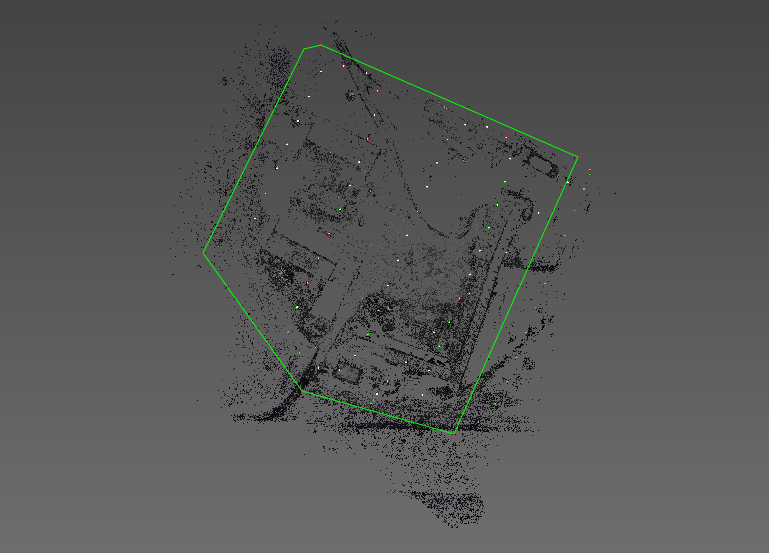
\includegraphics[width=0.4\linewidth]{FIGS/Viabon/masq3d.png}
    \end{center}
    \caption{Drawing a mask}
    \label{fig:sel}
\end{figure}

The {\tt mm3d PIMs} command is used to generate the digital surface model using the mode {\tt QuickMac}. The optional arguments {\tt Masq3D} and {\tt FilePair} are used to speed up the processing time cost.
\begin{verbatim}
mm3d PIMs QuickMac "image_002_00*.*tif" Ori-Compense-AF15P7-DPhase-La/ 
     Masq3D=AperiCloud_Compense-AF15P7-DPhase-La_polyg3d.xml 
     Out=NuageGps.ply FilePair=CpleImgs.xml
\end{verbatim}

We use {\tt mm3d PIMs2Mn} command to merge the result of the stereo depth maps computed above. The optional argument {\tt DoOrtho} is used to generate individual orthoimages.
\begin{verbatim}
mm3d PIMs2Mnt QuickMac DoOrtho=1
\end{verbatim}

The orthomosaic image is generated using the {\tt mm3d Tawny} command without performing any radiometric equalization.
\begin{verbatim}
Tawny PIMs-ORTHO/ RadiomEgal=false
\end{verbatim}

\begin{figure}[H]
    \begin{center}
    \setlength{\unitlength}{0.5cm}
    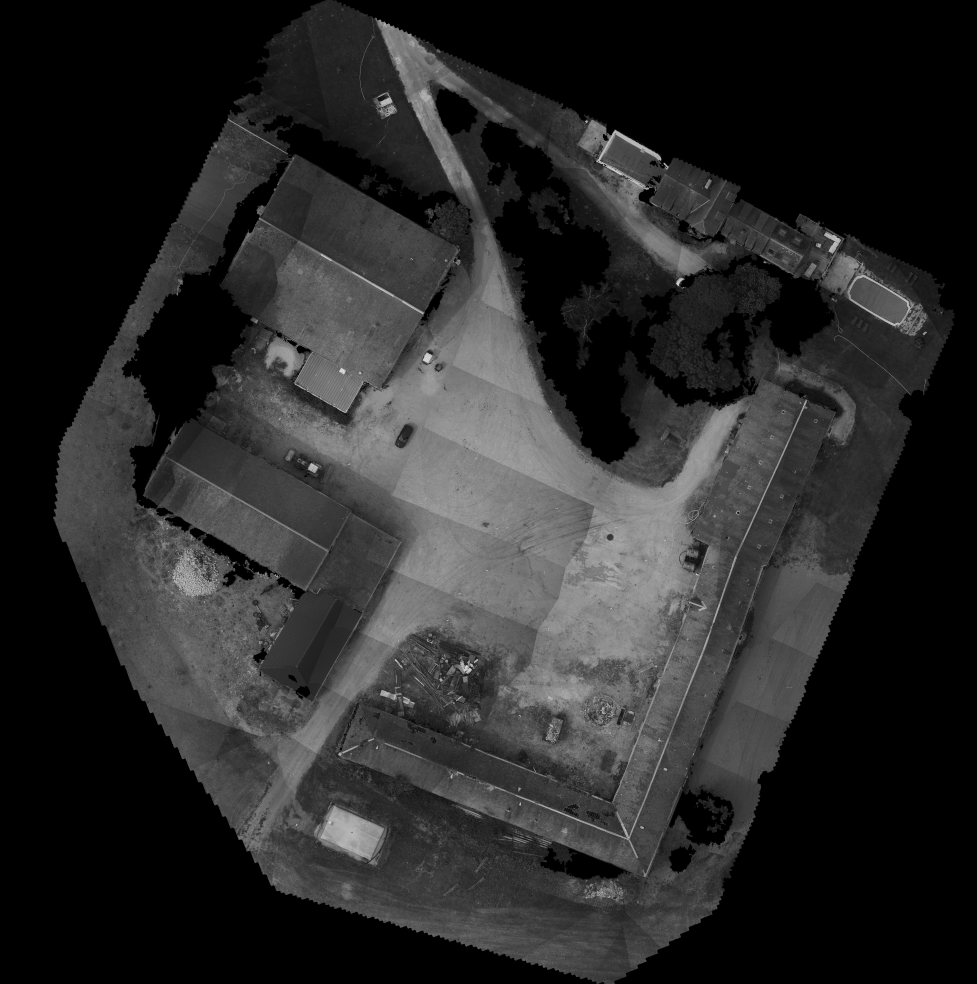
\includegraphics[width=0.4\linewidth]{FIGS/Viabon/ortho.png}
    \end{center}
    \caption{Orthoimage}
    \label{fig:sel}
\end{figure}

The shading image of depth map is computed using the {\tt mm3d Grshade} command.
\begin{verbatim}
mm3d Grshade PIMs-TmpBasc/PIMs-Merged_Prof.tif Out=Shading.tif ModeOmbre=IgnE
\end{verbatim}

\begin{figure}[H]
    \begin{center}
    \setlength{\unitlength}{0.5cm}
    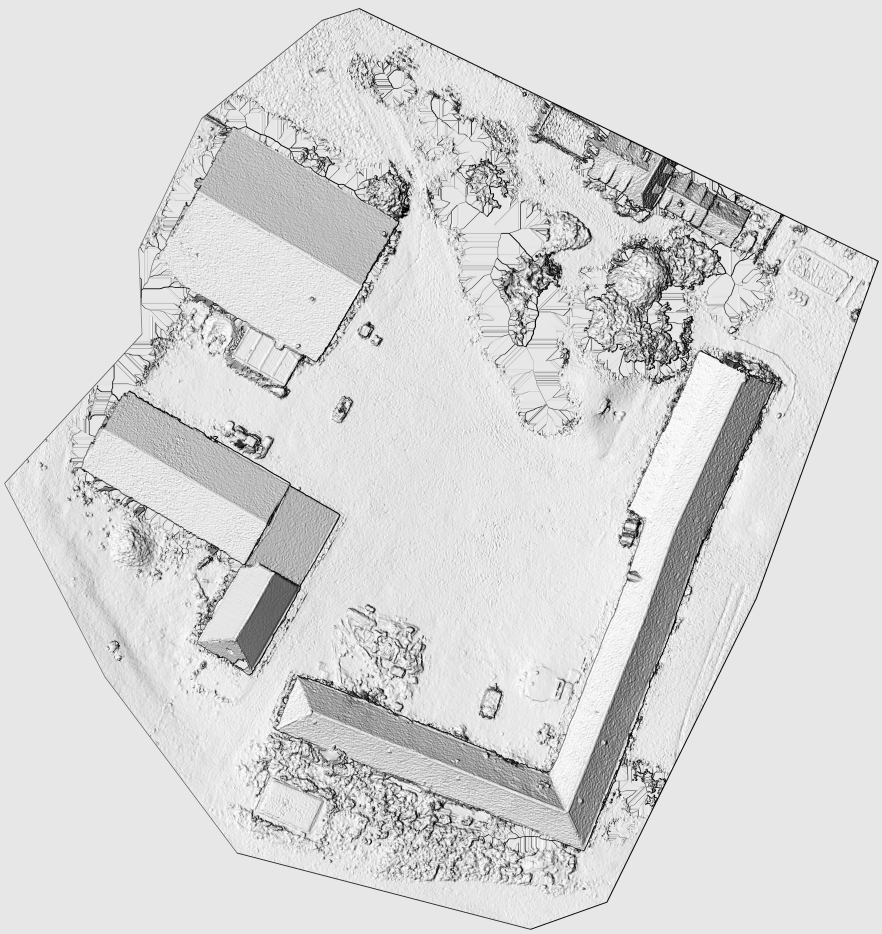
\includegraphics[width=0.4\linewidth]{FIGS/Viabon/shading.png}
    \end{center}
    \caption{Shading image}
    \label{fig:sel}
\end{figure}

To convert the depth map into a hypsometric representation we use the {\tt mm3d to8Bits} command.
\begin{verbatim}
mm3d to8Bits PIMs-TmpBasc/PIMs-Merged_Prof.tif Out=Hypso.tif Circ=1
\end{verbatim}

\begin{figure}[H]
    \begin{center}
    \setlength{\unitlength}{0.5cm}
    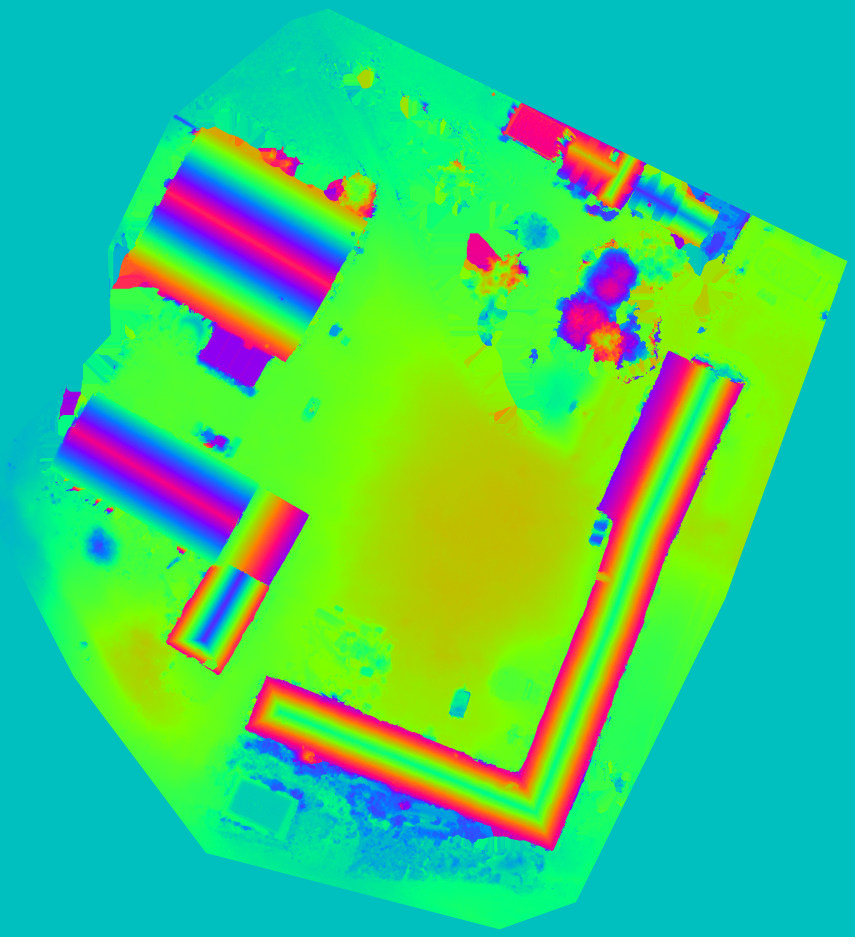
\includegraphics[width=0.4\linewidth]{FIGS/Viabon/hypso.png}
    \end{center}
    \caption{Hypsometric image}
    \label{fig:sel}
\end{figure}

The command {\tt mm3d Nuage2Ply} is used to export a dense points cloud.
\begin{verbatim}
mm3d Nuage2Ply PIMs-TmpBasc/PIMs-Merged.xml Scale=1 Attr=PIMs-ORTHO/Orthophotomosaic.tif 
     RatioAttrCarte=2 Out=GpsNuage.ply
\end{verbatim}

Visualization of the 3d points cloud using {\tt meshlab}.
\begin{verbatim}
meshlab GpsNuage.ply
\end{verbatim}
